\documentclass[12pt,letterpaper,reqno]{article}

% \usepackage{mathtools}
\usepackage{epsfig}
\usepackage{amsmath}
\usepackage{amssymb}
\usepackage{amsthm}
\usepackage{indentfirst}
\usepackage{xspace}
\usepackage{multirow}
\usepackage{hyperref}
\usepackage{xcolor}
\usepackage{verbatim}
\usepackage[letterpaper,margin=1in,headheight=15pt]{geometry}
\usepackage{mathpazo}
\usepackage{tikz-cd}
\usepackage{booktabs}
\usepackage{framed}
\usepackage{float}
\usepackage{thmtools}
\usepackage{dashrule}
\usepackage[missing=]{gitinfo2}
\usepackage{fancyhdr}
\usepackage{enumerate}
\usepackage{graphicx}
\usepackage{mathrsfs}
\usepackage{calligra}
\usepackage[titletoc,title]{appendix}

\definecolor{darkblue}{rgb}{0.1,0.1,0.7}
\definecolor{darkred}{rgb}{0.5,0.1,0.1}
\definecolor{darkgreen}{rgb}{0.0,0.42,0.06}
\hypersetup{colorlinks=true,urlcolor=darkred,linkcolor=darkblue,citecolor=darkred}
\definecolor{shadecolor}{rgb}{0.85,0.85,0.85}

% Bibliography formatting
\usepackage[bibstyle=authoryear-comp,labeldate=false,defernumbers=true,maxnames=20,uniquename=init,dashed=false,backend=biber,sorting=none]{biblatex}

\DeclareNameAlias{sortname}{first-last}

\DeclareFieldFormat{url}{\url{#1}}
\DeclareFieldFormat[article]{pages}{#1}
\DeclareFieldFormat[inproceedings]{pages}{\lowercase{pp.}#1}
\DeclareFieldFormat[incollection]{pages}{\lowercase{pp.}#1}
\DeclareFieldFormat[article]{volume}{\textbf{#1}}
\DeclareFieldFormat[article]{number}{(#1)}
\DeclareFieldFormat[article]{title}{\MakeCapital{#1}}
\DeclareFieldFormat[inproceedings]{title}{#1}
\DeclareFieldFormat{shorthandwidth}{#1}

% Don't use "In:" in bibliography. Omit urls from journal articles.
\DeclareBibliographyDriver{article}{%
  \usebibmacro{bibindex}%
  \usebibmacro{begentry}%
  \usebibmacro{author/editor}%
  \setunit{\labelnamepunct}\newblock
  \MakeSentenceCase{\usebibmacro{title}}%
  \newunit
  \printlist{language}%
  \newunit\newblock
  \usebibmacro{byauthor}%
  \newunit\newblock
  \usebibmacro{byeditor+others}%
  \newunit\newblock
  \printfield{version}%
  \newunit\newblock
%  \usebibmacro{in:}%
  \usebibmacro{journal+issuetitle}%
  \newunit\newblock
  \printfield{note}%
  \setunit{\bibpagespunct}%
  \printfield{pages}
  \newunit\newblock
  \usebibmacro{eprint}
  \newunit\newblock
  \printfield{addendum}%
  \newunit\newblock
  \usebibmacro{pageref}%
  \usebibmacro{finentry}}

% Remove dot between volume and number in journal articles.
\renewbibmacro*{journal+issuetitle}{%
  \usebibmacro{journal}%
  \setunit*{\addspace}%
  \iffieldundef{series}
    {}
    {\newunit
     \printfield{series}%
     \setunit{\addspace}}%
  \printfield{volume}%
%  \setunit*{\adddot}%
  \printfield{number}%
  \setunit{\addcomma\space}%
  \printfield{eid}%
  \setunit{\addspace}%
  \usebibmacro{issue+date}%
  \newunit\newblock
  \usebibmacro{issue}%
  \newunit}


% Bibliography categories
\def\makebibcategory#1#2{\DeclareBibliographyCategory{#1}\defbibheading{#1}{\section*{#2}}}
\makebibcategory{books}{Books}
\makebibcategory{papers}{Refereed research papers}
\makebibcategory{chapters}{Book chapters}
\makebibcategory{conferences}{Papers in conference proceedings}
\makebibcategory{techreports}{Unpublished working papers}
\makebibcategory{bookreviews}{Book reviews}
\makebibcategory{editorials}{Editorials}
\makebibcategory{phd}{PhD thesis}
\makebibcategory{subpapers}{Submitted papers}
\makebibcategory{curpapers}{Current projects}

\setlength{\bibitemsep}{2.65pt}
\setlength{\bibhang}{.8cm}
\renewcommand{\bibfont}{\small}

\renewcommand*{\bibitem}{\addtocounter{papers}{1}\item \mbox{}\hskip-0.85cm\hbox to 0.85cm{\hfill\arabic{papers}.~~}}
\defbibenvironment{bibliography}
{\list{}
  {\setlength{\leftmargin}{\bibhang}%
   \setlength{\itemsep}{\bibitemsep}%
   \setlength{\parsep}{\bibparsep}}}
{\endlist}
{\bibitem}

\newenvironment{publications}{\section{\LARGE Publications}\label{papersstart}\vspace*{0.2cm}\small
\titlespacing{\section}{0pt}{1.5ex}{1ex}\itemsep=0.00cm
}{\label{papersend}\addtocounter{sumpapers}{-1}\refstepcounter{sumpapers}\label{sumpapers}}

\def\printbib#1{\printbibliography[category=#1,heading=#1]\lastref{sumpapers}}

% Counters for keeping track of papers
\newcounter{papers}\setcounter{papers}{0}
\newcounter{sumpapers}\setcounter{sumpapers}{0}
\def\lastref#1{\addtocounter{#1}{\value{papers}}\setcounter{papers}{0}}

% theorem environments
\declaretheoremstyle[spaceabove=0.25cm,spacebelow=0.25cm,notefont=\normalfont\bfseries, notebraces={(}{)}]{theorem}
\declaretheoremstyle[spaceabove=0.25cm,spacebelow=0.25cm,bodyfont=\normalfont,notefont=\normalfont\bfseries, notebraces={(}{)}]{noital}
\declaretheoremstyle[spaceabove=0.25cm,spacebelow=0.25cm,bodyfont=\normalfont\color{darkgreen},notefont=\normalfont\bfseries, notebraces={(}{)}]{green}
\declaretheoremstyle[spaceabove=0.25cm,spacebelow=0.25cm,bodyfont=\normalfont,notefont=\normalfont\bfseries,qed=$\qedsymbol$,notebraces={(}{)}]{proofstyle}

\declaretheorem[name=Theorem,numberwithin=section,style=theorem]{thm}
\declaretheorem[name=Proposition,sibling=thm,style=theorem]{prop}
\declaretheorem[name=Corollary,sibling=thm,style=theorem]{cor}
\declaretheorem[name=Lemma,sibling=thm,style=theorem]{lem}
\declaretheorem[name=Definition,sibling=thm,style=noital]{defn}
\declaretheorem[name=Example,sibling=thm,style=noital]{example}
\declaretheorem[name=Exercise,numberwithin=section,style=green]{exercise}
\declaretheorem[name=Proof,style=proofstyle,numbered=no]{pf}

\numberwithin{equation}{section}


% macros for convenience
\newcommand{\tops}{\texorpdfstring}

\newcommand{\nid}{\noindent}

\newcommand{\fa}{{\mathfrak a}}
\newcommand{\fp}{{\mathfrak p}}
\newcommand{\fk}{{\mathfrak k}}
\newcommand{\fg}{{\mathfrak g}}
\newcommand{\fh}{{\mathfrak h}}
\newcommand{\fn}{{\mathfrak n}}
\newcommand{\fq}{{\mathfrak q}}
\newcommand{\fm}{{\mathfrak m}}
\newcommand{\fr}{{\mathfrak r}}
\newcommand{\fu}{{\mathfrak u}}
\newcommand{\fG}{{\mathfrak G}}

\newcommand{\cC}{\ensuremath{\mathcal C}}
\newcommand{\cG}{\ensuremath{\mathcal G}}
\newcommand{\cB}{\ensuremath{\mathcal B}}
\newcommand{\cL}{\ensuremath{\mathcal L}}
\newcommand{\cS}{\ensuremath{\mathcal S}}
\newcommand{\cF}{\ensuremath{\mathcal F}}
\newcommand{\cK}{\ensuremath{\mathcal K}}
\newcommand{\cZ}{\ensuremath{\mathcal Z}}
\newcommand{\cM}{\ensuremath{\mathcal M}}
\newcommand{\cN}{\ensuremath{\mathcal N}}
\newcommand{\cO}{\ensuremath{\mathcal O}}
\newcommand{\cH}{\ensuremath{\mathcal H}}
\newcommand{\cX}{\ensuremath{\mathcal X}}
\newcommand{\cY}{\ensuremath{\mathcal Y}}
\newcommand{\cA}{\ensuremath{\mathcal A}}
\newcommand{\cI}{\ensuremath{\mathcal I}}

\newcommand{\R}{\ensuremath{\mathbb R}}
\newcommand{\C}{\ensuremath{\mathbb C}}
\newcommand{\PP}{\ensuremath{\mathbb P}}
\newcommand{\Z}{\ensuremath{\mathbb Z}}
\newcommand{\Q}{\ensuremath{\mathbb Q}}
\newcommand{\A}{\ensuremath{\mathbb A}}
\newcommand{\bbH}{\ensuremath{\mathbb H}}
\newcommand{\bbI}{\ensuremath{\mathbb I}}
\newcommand{\bS}{\ensuremath{\mathbb S}}

\newcommand{\half}{\ensuremath{\frac{1}{2}}}
\newcommand{\qtr}{\ensuremath{\frac{1}{4}}}
\newcommand{\bq}{{\mathbf q}}
\newcommand{\N}{{\mathcal N}}
\newcommand{\F}{{\mathcal F}}
\newcommand{\HH}{{\mathcal H}}
\newcommand{\LL}{{\mathcal L}}
\newcommand{\RR}{{\mathcal R}}
\newcommand{\V}{{\mathcal V}}
\newcommand{\dirac}{\!\!\not\!\partial}
\newcommand{\Dirac}{\!\!\not\!\!D}
\newcommand{\cE}{{\mathcal E}}
\newcommand{\vs}{\not\!v}
\newcommand{\kahler}{K\"ahler\xspace}
\newcommand{\kq}{/\!\!/}
\newcommand{\kql}[1]{/\!\!/\!\!_#1\,}
\newcommand{\hk}{hyperk\"ahler\xspace}
\newcommand{\Hk}{Hyperk\"ahler\xspace}
\newcommand{\hkq}{/\!\!/\!\!/\!\!/}
\newcommand{\hkql}[1]{/\!\!/\!\!/\!\!/\!\!_#1\,}
\newcommand{\del}{\ensuremath{\partial}}
\newcommand{\delbar}{\ensuremath{\overline{\partial}}}
\newcommand{\I}{{\mathrm i}}
\newcommand{\J}{{\mathrm j}}
\newcommand{\K}{{\mathrm k}}
\newcommand{\e}{{\mathrm e}}
\newcommand\bid{{\mathbf 1}}
\newcommand{\de}{\mathrm{d}}
\newcommand{\ab}{\mathrm{ab}}
\newcommand{\vol}{\mathrm{vol}}
\renewcommand{\sf}{\mathrm{sf}}
\newcommand{\inst}{\mathrm{inst}}
\newcommand{\eff}{\mathrm{eff}}
\newcommand{\dR}{\mathrm{dR}}
\newcommand{\closed}{\mathrm{closed}}
\newcommand{\exact}{\mathrm{exact}}

\newcommand{\abs}[1]{\lvert#1\rvert}
\newcommand{\norm}[1]{\lVert#1\rVert}
\newcommand{\IP}[1]{\langle#1\rangle}
\newcommand{\DIP}[1]{\langle\!\langle#1\rangle\!\rangle}
\newcommand{\dwrt}[1]{\frac{\partial}{\partial#1}}
\newcommand{\eps}{\epsilon}
\newcommand{\simarrow}{\xrightarrow\sim}

\newcommand{\mmaref}[1]{}

\newcommand{\ti}[1]{\textit{#1}}
\newcommand{\tb}[1]{\textbf{#1}}
\newcommand{\lo}{\text{\calligra o}\,}
\newcommand{\dd}{\ensuremath{\mathscr{D}}}



\DeclareMathOperator{\ad}{ad}
\DeclareMathOperator{\im}{Im}
\DeclareMathOperator{\re}{Re}
\DeclareMathOperator{\Tr}{Tr}
\DeclareMathOperator{\End}{End}
\DeclareMathOperator{\Hom}{Hom}
\DeclareMathOperator{\Aut}{Aut}
\DeclareMathOperator{\Sym}{Sym}
\DeclareMathOperator{\Lie}{Lie}
\DeclareMathOperator{\diag}{diag}
\DeclareMathOperator{\Bun}{Bun}
\DeclareMathOperator{\Vect}{Vect}
\DeclareMathOperator{\Span}{Span}
\DeclareMathOperator{\grad}{grad}
\DeclareMathOperator{\rank}{rank}
\DeclareMathOperator{\ind}{ind}
\DeclareMathOperator{\coker}{coker}
\DeclareMathOperator{\Jac}{Jac}
\DeclareMathOperator{\Hol}{Hol}
\DeclareMathOperator{\gr}{gr}

\newcommand{\insfig}[2]{

\medskip
\noindent
\begin{minipage}{\linewidth}

\makebox[\linewidth]{\includegraphics[keepaspectratio=true,scale=#2]{figures/#1-crop.pdf}}

\end{minipage}
\medskip

}


% \newcommand{\insfig}[2]{\begin{figure}[htbp] \centering \includegraphics[scale=#2]{figures/#1-crop.pdf} \label{fig:#1} \end{figure}}
% syntax: \insfig{name}{0.5}{caption}

\newcommand{\fixme}[1]{{\color{orange}{[#1]}}}
\newcommand{\currentposition}{{\color{blue} \noindent\makebox[\linewidth]{\hdashrule{\paperwidth}{1pt}{3mm}}}}

% \mathtoolsset{showonlyrefs}

\bibliography{mvc}

\begin{document}
\pagestyle{fancy}
\lhead{{\tiny \color{gray} \tt \gitAuthorIsoDate}}
\chead{\tiny \ti{Multivariable Calculus, GSMST 2018-2019}}
\rhead{{\tiny \color{gray} \tt \gitAbbrevHash}}
\renewcommand{\headrulewidth}{0.5pt}


\begin{center}
\tb{Multivariable Calculus} \\
Anderson Trimm \\
Gwinnett School of Mathematics, Science and Technology 
\end{center}

{These are the notes for the 2018-2019
course in Multivariable Calculus at GSMST. They will continually be updated throughout the course. The latest PDF can always be found
at
\begin{center}
\small \url{https://github.com/atrimm/mvc/blob/master/Course%20Notes/mvc.pdf}
\end{center}
Please send corrections/improvements to
\begin{center}
\small \tt\href{mailto:anderson.trimm@gsmst.org}{anderson.trimm@gsmst.org}
\end{center}
or as pull requests to the source repository hosted at
\begin{center}
\small \url{https://github.com/atrimm/mvc}
\end{center}
}

\tableofcontents
\renewcommand{\listtheoremname}{Quick reference}
\listoftheorems[onlynamed]

\newpage

%\setcounter{page}{1}


\section{Introductory motivation}
\subsection{Review of single-variable calculus}
In single-variable calculus, one studies real-valued functions which depend on a single real-number variable, $x$. Denoting such a function as $y=f(x)$, one visualizes the function by drawing its graph in the $xy$-plane:
\begin{center}
	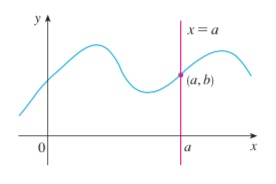
\includegraphics[scale=0.5]{figures_mvc/graph_of_a_function}
\end{center}
In terms of the graph, in single-variable calculus there are two main themes: the first is the \ti{tangent problem}, that is, to find the equation of the tangent line to the graph at a given point $P$.
\begin{center}
	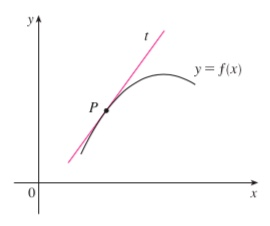
\includegraphics[scale=0.5]{figures_mvc/tangent_line_at_P}
\end{center}
The slope of the tangent line is the \ti{derivative} of the function, denoted by $f'(P)$ or $\frac{df}{dx}(P)$, and given by
\begin{align*}
	f'(P)=\lim_{t \to 0}\frac{f(P+t)-f(P)}{t},
\end{align*}
provided that this limit exists. The derivative $f'(P)$ has the interpretation as the \ti{instantaneous rate of change} of the function at $x=P$. We found the derivative very useful for \ti{optimization} problems, as a minimum or maximum of $f$ occurs where $f'=0$ (or on the boundary of the domain or at a point where $f'$ is not defined).

The second theme is the \ti{area problem}, that is, to find the area of a region bounded by the $x$-axis, the lines $(a,0)$ and $(b,0)$, and the graph of the function $f(x)$ (or, the \ti{signed area} if $f$ is not always positive on $[a,b]$). This area is given by the \ti{integral}
\begin{align*}
	\text{Area}=\int_a^b f(x)dx
\end{align*}
which is defined by breaking up this region into many thin rectangles and summing their areas. 
\begin{center}
	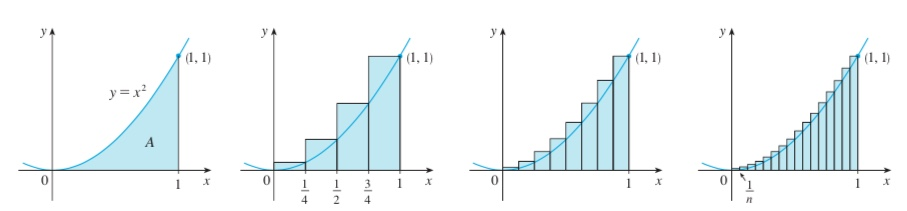
\includegraphics[scale=0.5]{figures_mvc/riemann_sum_example}
\end{center}
More precisely, we choose $n+1$ points $t_i$ such that $a=t_0<t_1<t_2<\cdots <t_{n-1}<t_n=b$ and a point $x_i^*$ in each interval $[t_{i-1},t_i]$, and define the integral to be the limit of the Riemann sum
\begin{align*}
	\int_a^b f(x)dx\equiv \lim_{n\to \infty} \sum_{i=0}^nf(x_i^*)(t_i-t_{i-1})
\end{align*}
again, provided that this limit exists. 

Recall that integrals are also useful for computing the length of the graph of $y=f(x)$ between two points 

\begin{center}
	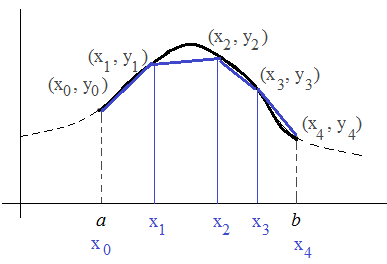
\includegraphics[scale=0.5]{figures_mvc/arc_length}
\end{center}asdf 

as well as the area of a surface of revolution.

\begin{center}
	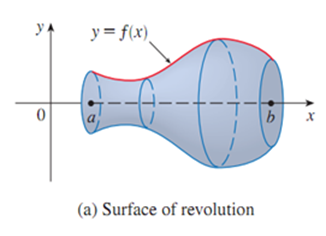
\includegraphics[scale=0.5]{figures_mvc/surface_of_revolution}
\end{center}


The \ti{fundamental theorem of calculus} tells us how these two problems are related. There are actually two versions:
\begin{enumerate}
	\item $\int_a^b f'(x)dx=f(b)-f(a)$ is the one which we use as a practical matter to compute integrals - we look for an antiderivative of the integrand, evaluate it at the two endpoints, and subtract.
	\item $\frac{d}{dx}\int_a^xf(t)dt=f(x)$ just says that the rate that the integral of $f$ changes as we change the upper limit of integration is given by $f(x)$ itself. This is intuitive, since increasing the upper limit by a small amount $\Delta x$ increases the area by approximately $f(x)\Delta x$, so dividing this by $\Delta x$ we are left with $f(x)$. This version is also very important since it is used to prove the first version.
\end{enumerate}

\subsection{Overview of multivariable calculus}
There are analogies to all of these problems in multivariable calculus. First of all, instead of restricting ourselves to functions $y=f(x)$ with one input and one output, we will consider functions which have either multiple inputs, multiple outputs, or both. 

As an example, the graph of a function of two variables, which we may denote as $z=f(x,y)$, is a surface in three-dimensional space with each output $z$ sitting over the input $(x,y)$.
\begin{center}
	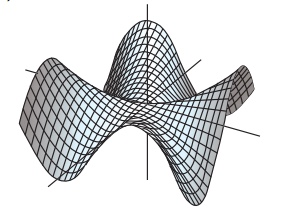
\includegraphics[scale=0.5]{figures_mvc/graph_of_z_of_x_y}
\end{center}
In this case, the analog of finding the equation of the tangent line to a curve at a given point is to find the equation of the tangent \ti{plane} to the surface at a given point.
\begin{center}
	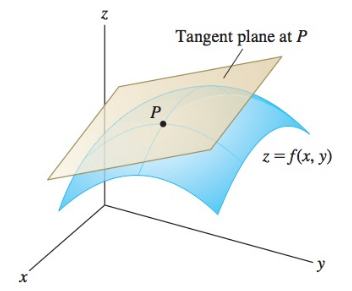
\includegraphics[scale=0.5]{figures_mvc/tangent_plane_example}
\end{center}

One quickly finds that optimization problems are far more rich in three dimensions. First of all, one can now compute the instantaneous rate of change of $z=f(x,y)$ in an infinite number of directions. The  slope of a tangent line to a surface is called a  \ti{partial derivative} of the function or, more generally, a \ti{directional derivative}.
\begin{center}
	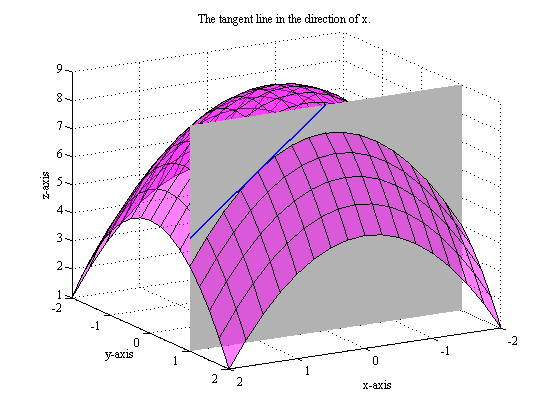
\includegraphics[scale=0.5]{figures_mvc/partial_derivative_2}
\end{center}
 Moreover, it is now possible that a critical point is a maximum in the $x$-direction, and a minimum in the $y$-direction, as in the example below.
\begin{center}
	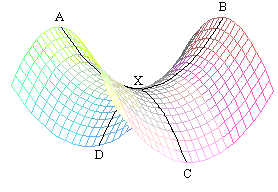
\includegraphics[scale=0.5]{figures_mvc/saddle_point}
\end{center}

The natural analogy of the problem in single-variable calculus of finding the area under a curve is to find the \ti{volume} under the graph of $z=f(x,y)$. This volume is also given by an integral, which is again defined as the limit of a Riemann sum, this time involving rectangular prisms.
\begin{center}
	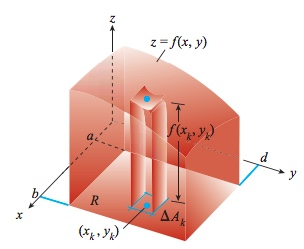
\includegraphics[scale=0.5]{figures_mvc/double_integral_example}
\end{center} 

We have just discussed a function with two inputs and one output, which we visualized as a surface in three-dimensions. We can also consider a function with one input and two (or three) outputs. In this case we get a \ti{vector-valued} function. Thinking of the input $t$ as time, at each instant of time the mapping gives us the three components of the vector ${\bf f}(t)=(f_1(t),f_2(t),f_3(t))$. The graph of this function is a \ti{curve} in three-dimensions, which might represent, say, the path of a particle. \footnote{Note that the vertical line test does not apply to this graph, since we are not looking at the graph of $z(x,y)$, but rather of $(x(t),y(t),z(t))$.}
\begin{center}
	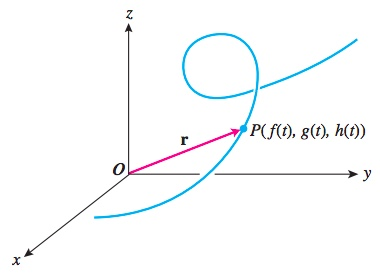
\includegraphics[scale=0.5]{figures_mvc/path_of_a_particle}
\end{center}

More generally, we can consider functions with three inputs \ti{and} three outputs. Such a function can still be visualized in three dimensions, as one can think of attaching a vector (the output) to each point in space (the input). Such a function is called a \ti{vector field}.
\begin{center}
	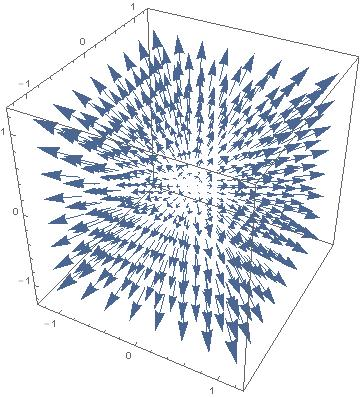
\includegraphics[scale=0.5]{figures_mvc/vector_field_example}
\end{center}

The culmination of the course will be the generalization of the fundamental theorem of calculus. In fact, we will actually talk about \ti{four} generalizations of the fundamental theorem of calculus. These are 
\begin{enumerate}
	\item The fundamental theorem of line integrals.
	\item Green's theorem.
	\item Stokes' theorem.
	\item The divergence theorem.
\end{enumerate}
Each of these theorems have many important applications. As an important example, Maxwell's equations, which lay the foundation of the classical theory of electromagnetism in the same way that Newton's laws of motion lay the foundation of classical mechanics, are stated in terms of these theorems. 

\subsection{Linear algebra}
As one might have guessed from the introductory discussion above, vectors play an essential role in the study of multivariable calculus. In effect, the theory of multivariable calculus unites single-variable calculus with the theory of \ti{linear algebra}, which includes the study of vectors, matrices, and linear transformations. To give a satisfactory treatment of multivariable calculus, the entire first semester of this course will therefore be devoted to the study of linear algebra. Aside from this motivation, the subject of linear algebra is rich and interesting in its own right, and has many diverse applications which are independent of differential and integral calculus. I hope to discuss many of these throughout the course.

\subsection{Mathematical structure}
The basic mathematical objects in linear algebra (vectors, scalars, matrices, etc.) have their origin in physics. While we will review these physical origins for the purpose of motivating the definitions, our primary objective in our study of linear algebra will be to build up an abstract mathematical structure called a \ti{vector space} and to study its properties. 

You already have experience in building mathematical structures in your previous courses. For instance, in algebra you defined various number systems along with an order and arithmetic on these sets of numbers. Then, you were then able to use logic to prove that these number systems had various interesting properties which followed inescapably from the definitions. You played exactly the same game in geometry, beginning with Euclid's axioms and the definitions of circles, triangles, parallelograms, etc., building up the entire structure of Euclidean geometry as theorems which follow as inescapable consequences of these rules and definitions.

The reason for emphasizing mathematical structure is that is that this is what is of paramount importance in mathematics, as once we determine the mathematical structure on a set of objects, the objects themselves become essentially \ti{irrelevant}. This is because whenever we find two sets which have the same mathematical structure, any conclusions about the first set which follow inescapably from this structure will hold \ti{verbatim} for the second set simply by replacing the names of the first objects by those of the second. This saves us an enormous amount of time as it prevents us from having to repeat all of the same computations for different concrete systems. 

Since this course will at many times mention ideas from physics, it is also worthwhile at this point to emphasize the difference between physics and mathematics. While as of the present moment physicists have found mathematics to be the only language which is capable of describing the laws of physics in a sufficiently detailed way, the objectives of physicists and mathematicians are very different. To put it shortly, one might say that physicists are interested in \ti{truth} whereas mathematicians are only interested in \ti{validity}. That is, in forming a mathematical structure (model), physicists create definitions and rules which they believe correspond to the \ti{real world}, that is, definitions and rules which, to the best of our knowledge, are \ti{true}. This approach to mathematics is often called \ti{applied mathematics}, i.e., practical mathematics. This is contrasted by what is called \ti{pure mathematics} (or, \ti{abstract mathematics}). A pure mathematician does not necessarily care at all whether the definitions and rules apply to the real world. He or she may define any consistent set of rules that they please, and apply the same logical reasoning to see what inescapable conclusions follow. That is, they are interested only in the logical process. If the theorems and propositions do indeed follow inescapably as a result of this logical process when applied to these axioms and definitions, then ones reasoning is said to be \ti{valid}, independently of whether the axioms and definitions bear any relation to the real world. \footnote{Note that truth (or at least what we believe to be true), unlike validity, is subject to change as we encounter new information. Both physicists and mathematicians are guided by the basic belief that if ones premises (assumptions) are true and ones argument is valid, then the conclusion must also be true. However, it is certainly possible that an argument can be valid and the conclusion be true even though the premises are \ti{false}. This is why no number of experiments can every prove a theory to be correct; the correct results could always be occurring despite wrong assumptions. This was true of the theory of classical mechanics. Despite having incorrect assumptions, Newton's theory of mechanics was consistent with all known experiments until the late 19th century when physicists first carried out new experiments which lead to the development of the theories of relativity and quantum mechanics. While at the present time these theories are in agreement with all known experiments, this could always change in the future.}

Of course, there is no structural difference between pure and applied mathematics,  the only difference being whether the mathematical model under consideration is believed to describe the real world. Moreover, the difference between pure and applied mathematics is often a time-dependent one, as a model that seemingly bears no relationship to the real world at present may eventually turn out to be a realistic model after all. For instance, instead of three-dimensional space, mathematicians like to consider $n$-dimensional space with $n>3$, even though the world only looks three-dimensional. This was pure mathematics until 1905 at which time Einstein introduced his theory of relativity, \footnote{Technically, this is the theory of \ti{special relativity}, which only deals with physics in unaccelerated reference frames. Einstein's \ti{general theory of relativity}, which turns out to be a relativistic theory of gravity, was introduced in 1915.} which showed that, fundamentally, there is a symmetry relating space and time, and that it is therefore more natural to formulate the laws of physics in a way in which space and time are on equal footing \footnote{This is exactly why the $x,y,$ and $z$-directions are treated identically, so that the consequences of the rotational symmetry relating them are made clear in our equations.}. That is, physical vectors are taken to belong to a certain \ti{four}-dimensional space called \ti{spacetime}.

\section{Vectors and geometry}
\subsection{Physical motivation}
The earliest notion of a \ti{vector} comes from physics. In nature, we encounter certain physical quantities, such as forces or velocities, which cannot be uniquely specified by a number alone, but also depend on a direction in space. 

\begin{example}
If the distance from town $A$ to town $B$ is 400 miles and we leave $A$ and travel at 50 miles per hour, then we will arrive at $B$ in 8 hours, but only if we travel in the direction from $A$ to $B$! Thus, displacement (400 mi, from $A$ to $B$) and velocity (50 mi/hr, from $A$ to $B$) are two examples of such physical quantities.
\end{example}
To distinguish physical quantities which depend on a numerical value alone from those which also depend on a direction, we make the following definitions. 
\begin{defn}[Vectors and scalars]
\begin{enumerate}[(a)] \hspace{10cm}
	\item A \ti{scalar} is a physical quantity which is uniquely specified by a numerical value alone.
	\item A \ti{vector} is a physical quantity which is uniquely specified by a numerical value, called its \ti{magnitude}, and a direction.
\end{enumerate}
\end{defn}
\subsection{Geometric interpretation}
A scalar can be represented geometrically as a distance on a number line, that is, by a  \ti{line segment}. For example, we think of the number 3 as a length of 3 units. Clearly, any two line segments of the same length represent the same scalar, so we are free to measure every line segment by positioning its left end at the origin of a number line.
\begin{center}
	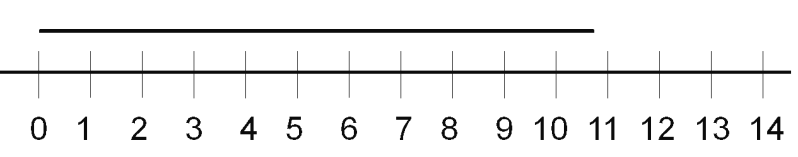
\includegraphics[scale=0.5]{figures_mvc/scalar_number_line}
\end{center}
A vector can therefore be represented as a \ti{directed} line segment, i.e., an arrow. As before, the length of the arrow will represent the magnitude of the vector. For example, if we wish to indicate a force of 2 pounds acting in the increasing \footnote{To represent a vector without ambiguity, when we specify the direction we must be sure to indicate the \ti{sense} of the vector. That is, in our present example, the word ``increasing'' denotes that we mean
\begin{center}
	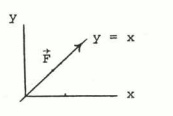
\includegraphics[scale=0.5]{figures_mvc/sense_1}
\end{center}
rather than
\begin{center}
	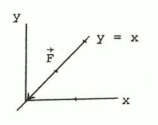
\includegraphics[scale=0.5]{figures_mvc/sense_2}
\end{center} In any diagram, it is therefore crucial to include the arrowhead to indicate the sense of the vector.} direction of the line $y=x$, we would represent it as the arrow ${\bf F}$.

\begin{center}
	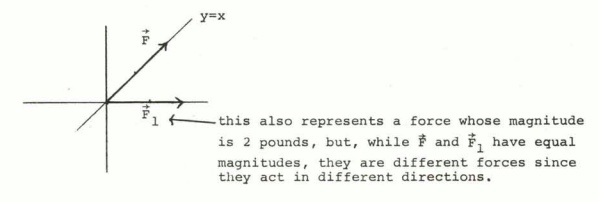
\includegraphics[scale=0.5]{figures_mvc/force_example}
\end{center}
The tail of the arrow is called the \ti{initial point} of the vector and the tip is called the \ti{terminal point}. 
\begin{center}
	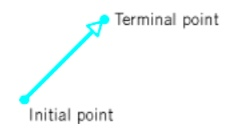
\includegraphics[scale=0.5]{figures_mvc/directed_line_segment}
\end{center}
We will denote a vector by boldface type, as in ${\bf v}$, and a scalar by lowercase italic type, as in $k$. When we want to indicate that a vector ${\bf v}$ has initial point $A$ and terminal point $B$, then we will write ${\bf v}=\overrightarrow{AB}$. \footnote{It is important to note that arrows are merely a convenient device to help us visualize vectors. That is, an arrow is a geometric representation of a vector, not the vector itself. Just as a number does not require the existence of a length, a vector require the existence of an arrow. Of course, once we have made this distinction, we may use vectors and arrows more or less interchangeably in the same way we use graphs and functions.}
\begin{center}
	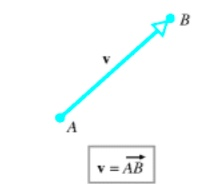
\includegraphics[scale=0.5]{figures_mvc/vAB}
\end{center}

\subsection{Vector arithmetic}
We have now defined a set of objects called vectors, which we visualize as arrows. To build a mathematical structure on this set, we need to define various rules and operations for working with vectors. As mathematicians, we are free to define any consistent set of rules and operations we like, and there are many possibilities.  Of course, our motivation for the introduction of vectors was to describe physical phenomena, and we will continue to take our motivations from physics in order to define a mathematical structure on the set of vectors.

\subsubsection{Equality of vectors}
The most basic rule is one which will allow us to determine when two vectors are equal. As we have taken a vector to have only two defining properties, namely its magnitude and direction, we will agree that
\begin{defn}[Equality of vectors]
Two vectors are equal if they have the same magnitude and direction.	
\end{defn}
In particular, this definition of equality means that if we have two distinct parallel line segments of the same length and we orient them with the same sense then these two vectors are equal.
\begin{center}
	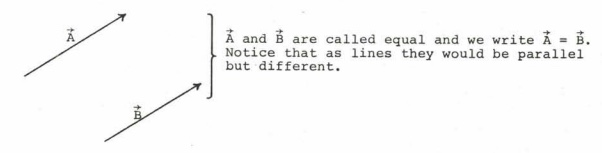
\includegraphics[scale=0.5]{figures_mvc/equal_vectors_new}
\end{center}
\begin{example}
A 2 second time interval and a 2 g mass are completely different physical quantities, their magnitude is exactly the same scalar, namely 2. Similarly, by our definition of equality of vectors, a velocity of 45 miles per hour along the increasing $y=x$ direction and a 45 $N$ force along the increasing $y=x$ direction are represented by exactly the same vector. \footnote{This is one of the reasons why mathematicians study abstract mathematical structures. Though one might have two sets of objects which look nothing alike, if they have the same mathematical structure, then any conclusions drawn about the first system hold \ti{verbatim} for the second system, simply by renaming the objects under consideration. This frees us from having to repeat the exact same mathematical computations for each concrete system we wish to consider; all we have to do is identify the mathematical structure of the set of objects we are studying, and then we know immediately that they behave exactly like every other set of objects which have the same mathematical structure.} 
\end{example}

\subsubsection{Vector addition}
Now that we know which vectors are distinct, our next step is to define operations on our set of vectors. The most basic operation is a \ti{binary operation}, which is a rule for combining any two vectors to produce a third. Exactly this kind operation can be studied in mechanics using a \ti{force table}.

\begin{center}
	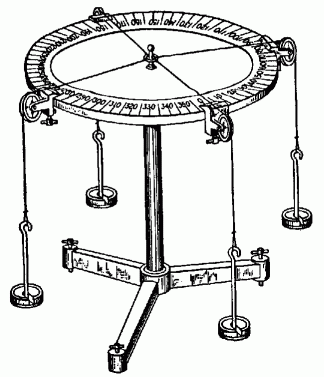
\includegraphics[scale=0.5]{figures_mvc/force_table_experiment_2}
\end{center}

In a force table experiment, strings are tied to a metal ring which is positioned at the center of the table. The strings are then suspended over pulleys which are fixed at known angles, and known masses hung from the ends of the strings. The pull of gravity on a given mass creates tension in the string which pulls on the washer. 

In an experiment in which \ti{two} strings are tied to the washer, the tension in each string gives rise to two forces pulling on the washer in different directions. However, the washer ultimately accelerates in a single direction, which is the direction of the \ti{net} (or \ti{total}) force acting on the washer. The rule for combining the two tension force vectors to produce the net force vector is exactly the binary operation we seek to define. Then, since we already have a definition which tells us when two vectors are equal, this rule will apply to \ti{all} vectors, whether they are forces, velocities, momenta, or any other type of vectors. 

To determine the net force, a third string is connected to the washer with pulley positioned and mass chosen so that the washer is in \ti{static equilibrium} (i.e., it does not move at all under the influence of these three forces). This vector is called the \ti{equilibrant} vector. By Newton's third law, the net force vector (also called the \ti{resultant} vector) is then the \ti{opposite} of the equilibrant vector, that is, it has the same magnitude and is directed along the same line, but with the opposite sense.

\begin{center}
	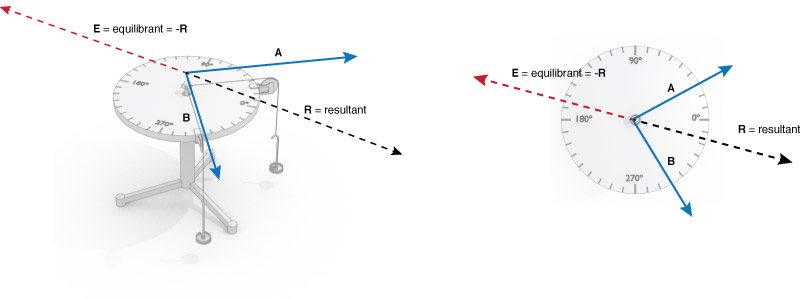
\includegraphics[scale=0.5]{figures_mvc/force-table-equi-res}
\end{center}

 We therefore define the \ti{sum} of two vectors as  
 
 \begin{defn}[Vector addition]
 	The \ti{sum} ${\bf v}+{\bf w}$ of two vectors ${\bf v}$ and ${\bf w}$ is the resultant vector of ${\bf v}$ and ${\bf w}$.
 \end{defn}
Note that when the two tension forces are along the \ti{same} direction, the resultant vector points in this same direction and has magnitude given by the sum of the magnitudes of the two tension vectors, and hence the addition of ${\bf v}$ and ${\bf w}$ reduces to addition of ordinary numbers in this special case. This is why we have decided to call this binary operation \ti{addition} and to continue to denote it by $+$; that is, it is a \ti{generalization} of ordinary addition. \footnote{To be completely rigorous and unambiguous, we should technically use some new symbol for this binary operation, such as ${\bf v}*{\bf w}$. However, it is standard practice to use the same symbol in such situations as it is conceptually useful to keep in mind the fact that this is a generalization of another operation.}
 
In terms of our geometric representation of vectors, the magnitude and direction of ${\bf v}+{\bf w}$ is determined as follows: Since the location of a vector is of no consequence (by our definition of equality of vectors), we may position the two vectors so that their initial points coincide. Then ${\bf v}$ and ${\bf w}$ form adjacent sides of a parallelogram, and the vector ${\bf v}+{\bf w}$ is the diagonal of the parallelogram, directed from the common initial point of ${\bf v}$ and ${\bf w}$ to the opposite vertex of the parallelogram, as shown below.	
\begin{center}
	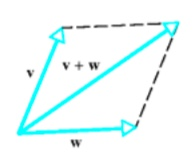
\includegraphics[scale=0.5]{figures_mvc/parallelogram_rule}
\end{center}
This is called the \ti{parallelogram rule} for vector addition. Since the opposite sides of a parallelogram are congruent and parallel, we can equivalently view ${\bf v}+{\bf w}$ as the result of positioning the initial point of ${\bf w}$ at the terminal point of ${\bf v}$ and drawing the arrow connecting the initial point of ${\bf v}$ to the terminal point of ${\bf w}$.

\begin{center}
	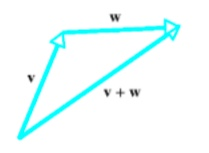
\includegraphics[scale=0.5]{figures_mvc/tip_to_tail}
\end{center}
This is called the \ti{triangle rule} or \ti{``tip to tail" rule} for vector addition. These two points of view are related by \ti{parallel translation}. To go from the first point of view to the second, we translate the initial point of ${\bf w}$ along ${\bf v}$, keeping ${\bf w}$ parallel to its original direction at all times. Accordingly, ${\bf v}+{\bf w}$ is also called the \ti{translation of ${\bf w}$ by ${\bf v}$}.
\begin{center}
	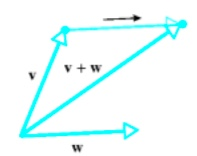
\includegraphics[scale=0.5]{figures_mvc/translation_of_v_by_w}
\end{center}
Let us emphasize once more that nothing forced us to choose this definition of vector addition, but by making this choice we are sure that our definition has at least one real interpretation, namely as the resultant vector in mechanics.

Let us now examine the properties of vector addition. Recall that the addition operation defined on the set of real numbers satisfies the following properties:
\begin{enumerate}[(a)]
	\item Commutativity: $x+y=y+x$ for all $x,y \in \mathbb{R}$.
	\item Associativity: $(x+y)+z=x+(y+z)$ for all $x,y,z \in \mathbb{R}$.
	\item Existence of an additive identity: $\mathbb{R}$ contains an element 0 such that $0+x=x$ for every $x \in \mathbb{R}$.
	\item Existence of additive inverses: For every $x \in \mathbb{R}$, there exists and element $y \in \mathbb{R}$ such that $x+y=0$.
\end{enumerate}
Let us use our definition of vector addition to consider each of these in turn.

\begin{prop}[Vector addition is commutative]
	Vector addition is commutative. That is, 
	\begin{align*}
		{\bf v}+{\bf w}={\bf w}+{\bf v}
	\end{align*}
	for any two vectors ${\bf v}$ and ${\bf w}$.
\end{prop}

\begin{pf}
	We see from the two diagrams below that the translation of ${\bf w}$ by ${\bf v}$ is the same vector as the translation of ${\bf v}$ by ${\bf w}$.
\begin{center}
	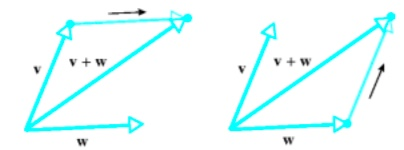
\includegraphics[scale=0.5]{figures_mvc/equivalence_of_vector_addition}
\end{center}

\end{pf}

\begin{prop}[Vector addition is associative]
	Vector addition is associative. That is, for any three vectors ${\bf u}, {\bf v},$ and ${\bf w}$, we have
	\begin{align*}
		{\bf u}+({\bf v}+{\bf w})=({\bf u}+{\bf v})+{\bf w}
	\end{align*}
We therefore denote both expressions by ${\bf u}+{\bf v}+{\bf w}$. 
\end{prop}

\begin{pf}
One can construct ${\bf u}+{\bf v}+{\bf w}$ by placing the vectors ``tip to tail" in succession and then drawing the vector from the initial point of ${\bf u}$ to the terminal point of ${\bf w}$. One can easily verify associativity from this construction, as shown below.
\end{pf}

\begin{center}
	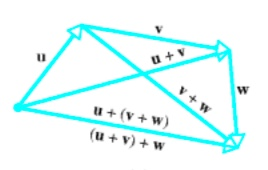
\includegraphics[scale=0.5]{figures_mvc/associativity_of_vector_addition}
\end{center}

The tip-to-tail method also makes it evident that if ${\bf u}, {\bf v},$ and ${\bf w}$ have a common initial point, then ${\bf u}+{\bf v}+{\bf w}$ is the diagonal of the parallelepiped that has the three vectors as adjacent sides.

\begin{center}
	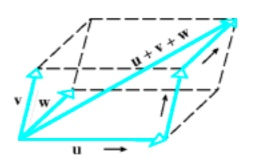
\includegraphics[scale=0.5]{figures_mvc/volume_of_parallelepiped_vectors}
\end{center}

\begin{cor}
The sum ${\bf v}_1+{\bf v}_2+\cdots + {\bf v}_k$ is independent of how the expression is bracketed.	
\end{cor}

\begin{pf}
As in the case of real numbers, the proof follows by induction on $k$. We will not repeat this here. \footnote{Of course, none of the proofs just presented are really proofs at all, since drawing pictures is not an acceptable substitute for airtight logic. For now, take them as plausibility arguments. We will prove these propositions rigorously in the next section.}	
\end{pf}

Let us now check whether there is a vector which plays the role of an additive identity. That is, given any vector ${\bf b}$, is there a vector ${\bf 0}$ such that ${\bf b}+{\bf 0}={\bf b}$? Let us suppose there is such a vector ${\bf 0}$ and denote its magnitude by $r$. Let us now add ${\bf 0}$ to ${\bf b}$ by the tip-to-tail method. Since ${\bf 0}$ has magnitude $r$, ${\bf b}+{\bf 0}$ must lie on a circle of radius $r$ centered on the tip of ${\bf b}$. However, the condition ${\bf b}+{\bf 0}={\bf b}$ means that ${\bf b}+{\bf 0}$ must have the same magnitude and direction as ${\bf b}$, and there is no point on the circle for which this is true. This shows that there is no such vector ${\bf 0}$ with nonzero length. 
\begin{center}
	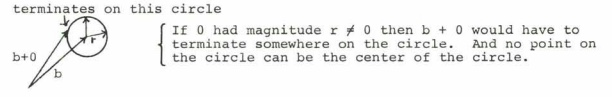
\includegraphics[scale=0.5]{figures_mvc/b_plus_zero_circle}
\end{center}

Thus, any vector of magnitude zero satisfies the requirement to serve as ${\bf 0}$, independently of direction. Now, for the real numbers, $0$ is unique, since if there are two numbers $0$ and $0'$ such that $x+0=x$ and $x+0'=x$ for all $x \in \mathbb{R}$, then $0=0+0'=0'$. However, our definition of equality of vectors says that two vectors of zero magnitude but different directions are not equal. Thus, if we want the zero vector to be unique, we must agree that we do not distinguish between two vectors of zero magnitude, even if they have different directions. This agrees with our geometric intuition, since a line segment of zero length is a point, which has no direction. Thus, with our modified definition of equality of vectors 

\begin{defn}[Equality of vectors ']
\begin{enumerate}[(1)] \hspace{10cm}
	\item Two nonzero vectors are equal if they have the same magnitude and direction.
	\item Any two vectors of zero magnitude are equal, even if their directions are different.
\end{enumerate}	
\end{defn}
and our definition of the zero vector
\begin{defn}[The zero vector]
	The zero vector, ${\bf 0}$, is any vector of zero magnitude.
\end{defn}
then ${\bf a}+{\bf b}$ is defined for \ti{any} two vectors ${\bf a}$ and ${\bf b}$, even if one is zero, and the zero vector ${\bf 0}$ is unique. \footnote{Note from our definition that the zero vector ${\bf 0}$ is not a single vector, but is actually a collection of vectors; namely, ${\bf 0}$ is the \ti{equivalence class} of all vectors with zero magnitude.}

Finally, we want to investigate whether, given any vector ${\bf a}$, we can find another vector ${\bf b}$ such that ${\bf a}+{\bf b}={\bf 0}$, where ${\bf 0}$ here denotes the zero vector. Since the zero vector has no length and since we add vectors from ``tip to tail", it follows that if ${\bf a}+{\bf b}={\bf 0}$, then the tail of ${\bf a}$ and the tip of ${\bf b}$ must coincide. This in turn means that ${\bf b}$ must have the same magnitude as ${\bf a}$ but opposite direction (directed along the same line, but with the opposite sense).  
\begin{center}
	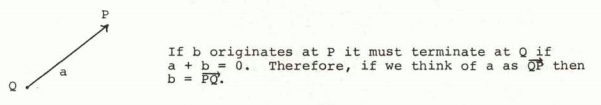
\includegraphics[scale=0.5]{figures_mvc/a_plus_b_equals_zero}
\end{center}
In other words, if we wish for vector addition to have the same structure as that of numerical addition, we \ti{must} define 
\begin{defn}[Inverse of a vector]
The additive inverse of ${\bf a}$ to be the vector which has the same magnitude, but opposite direction. 	
\end{defn}
In analogy with the equation $x+(-x)=0$ for real numbers, we denote the additive inverse of ${\bf a}$ by $-{\bf a}$, so that ${\bf a}+(-{\bf a})={\bf 0}$ for any vector ${\bf a}$. We may again agree, as in the case of numerical addition, to abbreviate ${\bf a}-{\bf b}$ as ${\bf a}-{\bf b}$, which allows us to define vector subtraction:

\begin{defn}[Vector subtraction]
	The difference ${\bf a}-{\bf b}$ of two vectors ${\bf a}$ and ${\bf b}$ is the sum
	\begin{align*}
		{\bf a}-{\bf b}={\bf a}+(-{\bf b}).
	\end{align*}
\end{defn}
From this definition, we may view vector subtraction geometrically as follows: To form ${\bf a}-{\bf b}$,
\begin{enumerate}[(1)]
	\item Obtain $(-{\bf b})$ from ${\bf b}$ by reversing the direction of ${\bf b}$.
	\item Add ${\bf a}$ and $(-{\bf b})$ in the usual way, by placing the tail of $(-{\bf b})$ at the tip of ${\bf a}$. \footnote{Like numerical subtraction, vector subtraction is \ti{not} commutative, so the order matters here.}
\end{enumerate}

\begin{center}
	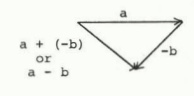
\includegraphics[scale=0.5]{figures_mvc/a_minus_b}
\end{center}

\begin{exercise}
Consider adding vectors ${\bf a}$ and ${\bf b}$ tail-to-tail, as shown below
	\begin{center}
		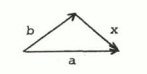
\includegraphics[scale=0.5]{figures_mvc/b_plus_x_equals_a}
	\end{center}
	Show that ${\bf x}={\bf a}-{\bf b}$. This gives another view of vector subtraction which is very useful computationally.
\end{exercise}

{\color{red} \flushleft {\bf Solution:}
We see from the tip-to-tail rule, that ${\bf b}+{\bf x}={\bf a}$. Adding $(-{\bf b})$ to both sides of this equation and using associativity gives ${\bf x}={\bf a}-{\bf b}$.}
The previous exercise shows that, if ${\bf a}$ and ${\bf b}$ are any two vectors and we wish to find ${\bf a}-{\bf b}$, we place the two vectors tail-to-tail and ${\bf a}-{\bf b}$ is then the vector which extends from the tip of ${\bf b}$ to the tip of ${\bf a}$.

We have just shown that our definition of vector addition satisfies the same properties as numerical addition. That is, the additive structures are exactly the same for vectors as for numbers. Therefore, any results that hold for numbers (with regard to addition) also hold for vectors, for exactly the same reasons. For example,

\begin{thm}[Cancellation law for vector addition]
	If ${\bf a}, {\bf b},$ and ${\bf c}$ are vectors such that ${\bf a}+{\bf b}={\bf a}+{\bf c}$, then ${\bf b}={\bf c}$. 
\end{thm}

\begin{pf}
The proof is exactly the same as for numbers (add $-{\bf a}$ to both sides), with the word ``vector" substituted for ``number".
\end{pf}

\subsubsection{Scalar multiplication}
In physics, we observe that an unbalanced force on a body causes an acceleration in the direction of the force. It is also observed that the magnitude of acceleration of different bodies, when subjected to the same force, varies according to their mass. These observations are formalized in Newton's second law of motion
\begin{equation}
	{\bf F}=m{\bf a}.
\end{equation}
On the right side of this equation, we see a new operation: the product of a scalar and a vector. Due to the fundamental nature of Newton's second law, if we want to build a mathematical structure which is capable of describing nature, we should include this operation.

\begin{defn}[Scalar multiplication]
The \ti{scalar multiple} of the vector ${\bf v}$ by the scalar ${\bf k}$ is the vector ${\bf w}=k{\bf v}$. The length of ${\bf w}$ is $|k|$ times the length of ${\bf v}$. If $k>0$, ${\bf w}$ points in the same direction as ${\bf v}$, while if $k<0$, ${\bf w}$ points in the direction of $-{\bf v}$. If $k=0$ or ${\bf v}={\bf 0}$, then we defined $k{\bf v}$ to be ${\bf 0}$.
\end{defn}

\begin{center}
	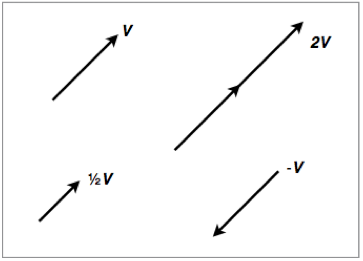
\includegraphics[scale=0.5]{figures_mvc/scalar_mult_examples}
\end{center}

\begin{example}
The vector $2{\bf v}$ has the same direction as ${\bf v}$ but twice its length, while $-2{\bf v}$ is oppositely directed to ${\bf v}$ and twice its length.	
\end{example}

\begin{prop}[Properties of scalar multiplication]\label{prop:Properties_of_scalar_multiplication}
For any scalars $c,d$ and vectors ${\bf v}, {\bf w}$,
	\begin{enumerate}[(a)]
		\item 1{\bf v}={\bf v},
		\item 0{\bf v}={\bf 0},
		\item $(-1){\bf v}=-{\bf v}$,
		\item $(dc){\bf v}=c(d{\bf v})$,
		\item $(c+d){\bf v}=c{\bf v}+d{\bf v}$,
		\item $c({\bf v}+{\bf w})=c{\bf v}+c{\bf w}$.
	\end{enumerate}
\end{prop}

\begin{exercise}
Prove Proposition \ref{prop:Properties_of_scalar_multiplication}. \\
\ti{Hints for (e) and (f):}
\begin{enumerate}[(a)]
\setcounter{enumi}{4}
	\item This follows from the segment addition postulate (it will help to start by drawing a picture). You will need to consider the different sign combinations for $c$ and $d$. Don't forget the cases where $c$ or $d$ is zero.
	\item This follows from similar triangles (again, start by drawing a picture).
\end{enumerate}
\end{exercise}


\subsection{Vectors in coordinate systems}
As in analytic geometry, the use of coordinate systems give us powerful tools with which to perform concrete computations with vectors. Additionally, working with coordinates will allow us to consider geometric entities such as lines and planes in vector settings. 

\subsubsection{Coordinate correspondence}
In this section we describe the coordinate correspondence between three-dimensional Euclidean space, $\mathbb{E}^3$ (the three-dimensional space in which the axioms of Euclidean geometry hold), and three-dimensional Cartesian space $\mathbb{R}^3\equiv \{(x_1,x_2,x_3):x_i \in \mathbb{R} \text{ for } i=1,2,3\}$.

We begin with a line. A coordinate correspondence between a line $L$ and the real number system $\mathbb{R}$ is determined by choosing arbitrarily on $L$ a zero point $O$ and a unit point $Q$ distinct from $O$. Then to each point $X$ on $L$ is assigned the number $x$ such that $|x|$ is the distance from $O$ to $X$, measured in terms of the segment $OQ$ as the unit, and $x$ is positive or negative according to whether $X$ and $Q$ are on the same side of $O$ or on opposite sides. The mapping $X \mapsto x$ is the coordinate correspondence between $L$ and $\mathbb{R}$. 

We now set up a coordinate correspondence between $\mathbb{E}^3$ and $\mathbb{R}^3$. We first choose arbitrarily a zero point $O$ and three unit points $Q_1, Q_2,$ and $Q_3$ in such a way that the four points do not lie in a plane. Each of the unit points $Q_i$ determines a line $L_i$ through $O$ and a coordinate correspondence on this line, as defined above. The three lines $L_1, L_2$, and $L_3$ are called the \ti{coordinate axes}. Consider now any point $X$ in $\mathbb{E}^3$. The plane through $X$ parallel to $L_2$ and $L_3$ intersects $L_1$ at a point $X_1$, and therefore determines a number $x_1$, the coordinate of $X_1$ on $L_1$. Similarly, $X$ determines points $X_2$ on $L_2$ and $X_3$ on $L_3$ which have coordinates $x_2$ and $x_3$, respectively. Altogether, $X$ determines a triple
\begin{align*}
	{\bf x}=(x_1,x_2,x_3)
\end{align*} 
in $\mathbb{R}^3$, and we have thus defined a mapping $\theta:X \mapsto {\bf x}$ from $\mathbb{E}^3$ to $\mathbb{R}^3$. 

\begin{center}
	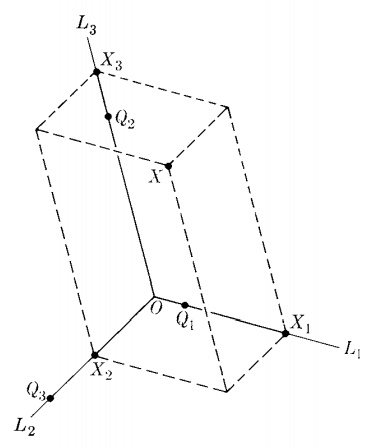
\includegraphics[scale=0.5]{figures_mvc/e3_r3}
\end{center}
We call $\theta$ the \ti{coordinate correspondence} defined by the axis system. Note that the unit point $Q_1$ on $L_1$ has the coordinate triple $(1,0,0)$, and similarly
\begin{align*}
	\theta(Q_2)&=(0,1,0), \\
	\theta(Q_3)&=(0,0,1).
\end{align*}

It is a fact that $\theta$ is a bijection from $\mathbb{E}^3$ to $\mathbb{R}^3$. \footnote{The proof uses techniques beyond the usual treatment of high school geometry, so we will simply accept this statement without proof.} The power of this one-to-one correspondence is that it allows us treat geometric questions algebraically.

\subsubsection{Cartesian coordinates}
\begin{defn}[Cartesian coordinates]
	The axis system in $\mathbb{E}^3$ is \ti{Cartesian} if the coordinate axes are mutually perpendicular and a common unit of distance (i.e., $|OQ_1|=|OQ_2|=|OQ_3|$) is used. The corresponding coordinates are called \ti{Cartesian coordinates}.
\end{defn}
A Cartesian coordinate system is shown below. \footnote{Cartesian coordinates are also often called \ti{rectangular coordinates} because the axes that define them meet at right angles.}
\begin{center}
	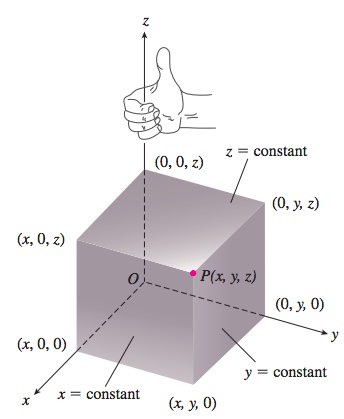
\includegraphics[scale=0.5]{figures_mvc/cartesian_coordinate_system}
\end{center}
The coordinate axes are labeled $x,y,$ and $z$, and are arranged such that if you take your right hand and curl your fingers from the positive $x$-axis toward the positive $y$-axis, your thumb points along the positive $z$-axis. Such a coordinate system is called \ti{right-handed}. \footnote{As you might have guessed, there are also left-handed coordinate systems. Choosing our coordinate system to be left- or right-handed is called choosing an \ti{orientation} for our coordinate system. We will discuss orientations more later. For now, just note that everything we do in the following could equivalently be formulated in terms of left-handed coordinate systems, so choosing a right-handed coordinate system for $\mathbb{E}^3$ is simply the standard convention.}

As discussed in the previous section, the coordinates of a point $P$ are the numbers at which the planes through $P$ perpendicular to the coordinate axes intersect these axes. These are labeled $\theta(P)=(x,y,z)$. 

Points on the $x$-axis have $y$- and $z$-coordinates equal to zero. That is, they have coordinates of the form $(x,0,0)$. Similarly points on the $y$- and $z$-axes have coordinates of the from $(0,y,0)$ and $(0,0,z)$, respectively.

The points in a plane perpendicular to the $x$-axis all have the same $x$-coordinate, $x_0$, this being the number at which the plane intersects that $x$-axis. The plane is then the set 
\begin{equation}
	P=\{(x,y,z) \in \mathbb{R}^3 : x=x_0\} 
\end{equation}
That is, the plane consists of all points having coordinates $(x_0,y,z)$, where $y$ and $z$ are any real numbers. The constraint $x=x_0$ is the equation of the plane perpendicular to the $x$-axis and intersecting it at $x_0$. Similar formulas hold for planes perpendicular to the $y$- and $z$-axes.

\begin{example}
The plane $x=2$ is the plane perpendicular to the $x$-axis at $x=2$. The plane $y=3$ is the plane perpendicular to the $y$-axis at $y=3$. The plane $z=5$ is the plane perpendicular to the $z$-axis at $z=5$. These planes are shown below, together with their intersection point $(2,3,5)$.
\end{example}

\begin{center}
	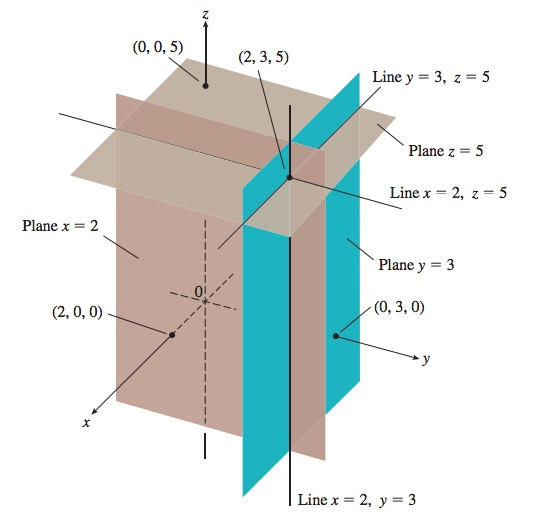
\includegraphics[scale=0.5]{figures_mvc/plane_235}
\end{center}

The planes $x=2$ and $y=3$ in the figure above intersect along a line parallel to the $z$-axis. This line is described by a pair of equations $L=\{(x,y,z) \in \mathbb{R}^3: x=2 \text{ and } y=3\}$.

\begin{exercise}
	Describe the other two lines of intersection in the figure above.
\end{exercise}

{\color{red} \flushleft {\bf Solution:}
The line running parallel to the $x$-axis is given by $$L_1=\{(x,y,z) \in \mathbb{R}^3: y=3 \text{ and } z=5\},$$ while the line running parallel to the $y$-axis is given by $$L_2=\{(x,y,z) \in \mathbb{R}^3: x=2 \text{ and } z=5\}.$$}

The three planes determined by the coordinate axes are the $xy$-plane, whose equation is $z=0$; the $yz$-plane, whose equation is $x=0$; and the $xz$-plane, whose equation is $y=0$. They meet at the origin, $(0,0,0)$.
	
The three coordinate planes $x=0, y=0,$ and $z=0$ divide space into eight cells called \ti{octants}. The octant in which the coordinates of all points are nonnegative is called the \ti{first octant}; there is no conventional numbering for the other seven octants.

\begin{exercise}
Write the coordinate equations and inequalities which define each of the following sets of points in space.
\begin{enumerate}[(a)]
	\item The half-space consisting of the points on and above the $xy$-plane.
	\item  This plane is parallel to the $yz$-plane and lying 3 units behind it.
	\item The second quadrant of the $xy$-plane.
	\item The first octant.
	\item The slab between the planes $y=-1$ and $y=1$, including these planes.
	\item The line in which the planes $y=-2$ and $z=2$ intersect.
\end{enumerate}	
\end{exercise}

{\color{red} \flushleft {\bf Solution:} 
\begin{enumerate}[(a)]
	\item $z \geq 0$,
	\item $x=-3$,
	\item $z=0, x \leq 0, z \geq 0$,
	\item $x \geq 0, y \geq 0, z \geq 0$,
	\item $-1 \leq y \leq 1$,
	\item $y=-2,z=2$.
\end{enumerate}}

\begin{exercise}
	What points $P(x,y,z)$ satisfy the equations
	\begin{align*}
		x^2+y^2=4 \text{ and }z=3?
	\end{align*}
\end{exercise}

{\color{red} \flushleft {\bf Solution:} These equations describe a circle of radius 2 lying in a plane parallel to the $xy$-plane and lying 3 units above it.}

\begin{center}
	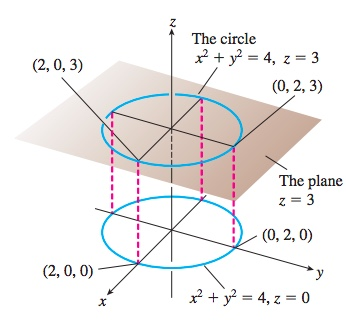
\includegraphics[scale=0.5]{figures_mvc/circle_z=3}
\end{center}

\subsubsection{Components of a vector}
Let us choose a Cartesian coordinate system for three-dimensional space. If a vector is positioned with its initial point at the origin, then the vector is completely determined by the coordinates of its terminal point.

\begin{center}
	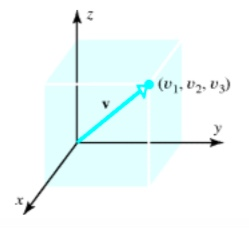
\includegraphics[scale=0.5]{figures_mvc/components}
\end{center}

\begin{defn}[Components of a vector]
	The coordinates of the terminal point of a vector ${\bf v}$ positioned with its initial point at the origin are called the \ti{components} of ${\bf v}$. We denote the components of a vector ${\bf v}$ by writing ${\bf v}=(v_1,v_2,v_3)$.
\end{defn}

\subsection{Norm of a vector}
In Cartesian coordinates, we can easily compute the length of a vector in terms of its components. The length of a vector is also called its \ti{norm}. 
\begin{defn}[Norm of a vector]\label{def:length_of_a_vector}
	The \ti{norm} of a vector ${\bf v}$, denoted $||{\bf v}||$, is given in terms of its Cartesian coordinates by
	\begin{align*}
		||{\bf v}||=\sqrt{v_1^2+v_2^2+v_3^2}.
	\end{align*}
\end{defn}

\begin{pf}
This formula follows directly from the Pythagorean theorem. In the diagram below,
\begin{center}
	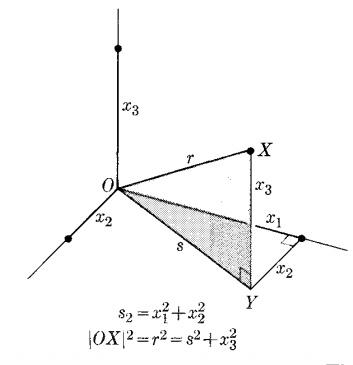
\includegraphics[scale=0.5]{figures_mvc/euclidean_norm}
\end{center}	
we see from the right triangle in the $x_1x_2$-plane that that $s^2=x_1^2+x_2^2$. Then, from triangle $XYO$, we have $r^2=s^2+x_3^2=x_1^2+x_2^2+x_3^2$.
\end{pf}

We also think of the norm as a function which takes in a vector and returns its length. This function has the following properties.

\begin{prop}[Norm properties]
	For any scalar $a$ and any vectors ${\bf v}$ and ${\bf w}$,
	\begin{enumerate}[(1)]
		\item $||{\bf v}|| \geq 0$, ${\bf v}={\bf 0}$ if and only if ${\bf v}={\bf 0}$. (positive-definite)
		\item $||a{\bf v}||=|a| \ ||{\bf v}||$ (homogeneity)
	\end{enumerate}
\end{prop}

\begin{pf}
\begin{enumerate}[(a)]
	\item $||{\bf v}||=\sqrt{v_1^2+v_2^2+v_3^2}$ is a nonnegative function and zero if and only if $v_1=v_2=v_3=0$, that is, if ${\bf v}={\bf 0}$.
	\item $||a{\bf v}||=\sqrt{a^2v_1^2+a^2v_2^2+a^2v_3^2}=\sqrt{a^2(v_1^2+v_2^2+v_3^2)}=\sqrt{a^2}\sqrt{(v_1^2+v_2^2+v_3^2)}=|a|\||{\bf v}||$.
\end{enumerate}
\end{pf}


\begin{defn}[Unit vector]
	A \ti{unit vector} is a vector of unit length. That is, a vector ${\bf v}$ such that $||{\bf v}||=1$.
\end{defn}

\begin{prop}[Normalizing a vector]
	If ${\bf v}\neq 0$, then ${\bf v}/||{\bf v}||$ is a unit vector in the direction of ${\bf v}$. The unit vector ${\bf v}/||{\bf v}||$ is often denoted ${\bf \hat{v}}$ and the process of forming ${\bf \hat{v}}$ from ${\bf v}$ is called \ti{normalizing} ${\bf v}$.
\end{prop}

\begin{pf}
Since ${\bf v}\neq 0$, $||{\bf v}|| \neq 0$, so we can multiply ${\bf v}$ by $1/||{\bf v}||$. Computing the length of $||\frac{{\bf v}}{||{\bf v}||}||$, we see that 
\begin{align*}
	||\frac{{\bf v}}{||{\bf v}||}||&=\frac{||{\bf v}||}{||{\bf v}||}=1,
\end{align*} 
hence ${\bf v}/||{\bf v}||$ is a unit vector. Since ${\bf v}/||{\bf v}||$ is a scalar multiple of ${\bf v}$ (by $k=1/||{\bf v}||$) it is parallel to ${\bf v}$.
\end{pf}

\begin{example}
	We can express any nonzero vector ${\bf v}$ as a product of its magnitude and direction by means of the formula
	\begin{align*}
		{\bf v}=||{\bf v}||\frac{{\bf v}}{||{\bf v}||}.
	\end{align*}
	For example, taking ${\bf v}=(1,-2,3)$,
	\begin{align*}
		||{\bf v}||=\sqrt{1^2+(-2)^2+3^2}=\sqrt{14}
	\end{align*}
	and thus
	\begin{align*}
		{\bf v}=\sqrt{14}(\frac{1}{\sqrt{14}},\frac{-2}{\sqrt{14}},\frac{3}{\sqrt{14}}).
	\end{align*}
\end{example}


\begin{defn}[Standard unit vectors]
	 The \ti{standard unit vectors} for $\mathbb{E}^3$ are the vectors
	\begin{align*}
		{\bf e}_1&=(1,0,0), \\
		{\bf e}_2&=(0,1,0), \\
		{\bf e}_3&=(0,0,1). \\
	\end{align*}
These vectors are unit vectors pointing along the $x$-, $y$-, and $z$-axes, respectively. \footnote{The standard unit vectors $({\bf e}_1,{\bf e}_2,{\bf e}_3)$ are also commonly denoted as $({\bf i}, {\bf j}, {\bf k})$ or $({\bf \hat{x}}, {\bf \hat{y}}, {\bf \hat{z}})$.}	
\end{defn}
Using the standard unit vectors, we may write the vector ${\bf v}=(v_1,v_2,v_3)$ as $${\bf v}=v_1{\bf e}_1+v_2{\bf e}_2+v_3{\bf e}_3.$$

\begin{prop}[Vector operations in coordinates]
	Let ${\bf v}=(v_1,v_2,v_3)$ and ${\bf w}=(w_1,w_2,w_3)$ be vectors and $k$ a scalar. Then
	\begin{align*}
		{\bf v}+{\bf w}&=(v_1+w_1,v_2+w_2,v_3+w_3), \\
		{\bf v}-{\bf w}&=(v_1-w_1,v_2-w_2,v_3-w_3), \\
		k{\bf v}&=(kv_1,kv_2,kv_3).
	\end{align*}
\end{prop}

\begin{pf}
These formulas can be seen by examining the following diagrams.
\begin{center}
	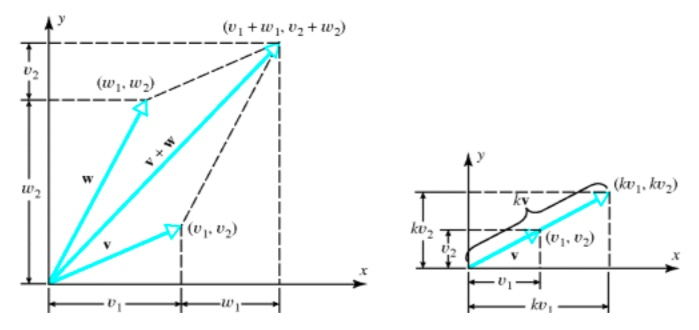
\includegraphics[scale=0.5]{figures_mvc/vector_operations}
\end{center}	
\end{pf}

\begin{prop}[Vector from one point to another]\label{prop:vector_from_one_point_to_another}
	The vector from $P_1(x_1,y_1,z_1)$ to $P_2(x_2,y_2,z_2)$ is given by
	\begin{align*}
		\overrightarrow{P_1P_2}=(x_2-x_1,y_2-y_1,z_2-z_1).
	\end{align*}
\end{prop}

\begin{pf}
From the figure below, 
\begin{center}
	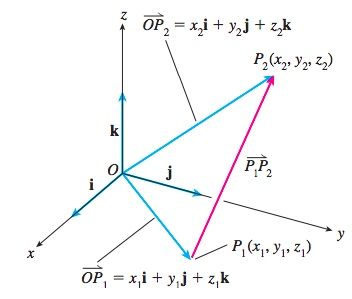
\includegraphics[scale=0.5]{figures_mvc/P1P2}
\end{center}

we see that $\overrightarrow{OP_1}+\overrightarrow{P_1P_2}=\overrightarrow{OP_2}$, and therefore
\begin{align*}
	\overrightarrow{P_1P_2}&=\overrightarrow{OP_2}-\overrightarrow{OP_1} \\
	&=(x_2,y_2,z_2)-(x_1,y_1,z_1) \\
	&=(x_2-x_1,y_2-y_1,z_2-z_1).
\end{align*}	
\end{pf}

\begin{cor}[Distance between two points]
	The distance between two points $P_1(x_1,y_1,z_2)$ and $P_2(x_2,y_2,z_2)$ is given by
	\begin{align*}
		||\overrightarrow{P_1P_2}||=\sqrt{(x_2-x_1)^2+(y_2-y_1)^2+(z_2-z_1)^2}.
	\end{align*}
\end{cor}

\begin{pf}
	This formula follows immediately from Prop. \ref{prop:vector_from_one_point_to_another} and Def. \ref{def:length_of_a_vector}.
\end{pf}

\begin{exercise}
\begin{enumerate}[(a)]
	\item Find the components of the vector $\overrightarrow{P_1P_2}$ with initial point $P_1(2,-1,4)$ and terminal point $P_2(7,5,-8)$.
	\item Find the distance between $P_1(2,-1,4)$ and $P_2(7,5,-8)$.
\end{enumerate}	
\end{exercise}

{\color{red} \flushleft {\bf Solution:} 
\begin{enumerate}[(a)]
	\item The components of $\overrightarrow{P_1P_2}$ are given by
	\begin{align*}
		\overrightarrow{P_1P_2}=(7-2,5-(-1),-8-4)=(5,6,-12)
	\end{align*}
	\item The distance between $P_1$ and $P_2$ is 
	\begin{align*}
		||\overrightarrow{P_1P_2}||=\sqrt{5^2+6^2+(-12)^2}=\sqrt{205}.
	\end{align*}
\end{enumerate}}

\begin{exercise}
Find a unit vector in the direction of the vector from $P_1(1,0,1)$ to $P_2(3,2,0)$.
\end{exercise}

{\color{red} \flushleft {\bf Solution:}
We find $\overrightarrow{P_1P_2}$ and normalize:
\begin{align*}
	\overrightarrow{P_1P_2}&=(3-1,2-0,0-1)=(2,2,-1), \\
	||\overrightarrow{P_1P_2}||&=\sqrt{2^2+2^2+(-1)^2}=3, \\
\end{align*}
and therefore the desired unit vector is given by
\begin{align*}
	\frac{\overrightarrow{P_1P_2}}{||\overrightarrow{P_1P_2}||}=(\frac{2}{3},\frac{2}{3},-\frac{1}{3}).
\end{align*}}

\begin{exercise}
Find a vector 6 units long in the direction of ${\bf v}=(2,2,-1)$.	
\end{exercise}

{\color{red} \flushleft {\bf Solution:}
The vector we want is 
\begin{align*}
6\frac{{\bf v}}{||{\bf v}||}=6\frac{(2,2,-1)}{\sqrt{2^2+2^2+(-1^2)}}=6\frac{(2,2,-1)}{3}=(4,4,-2).	
\end{align*}
}

\begin{exercise}
	A sphere of radius $r$ centered at $(x_0,y_0,z_0)$ is the set of all points in $\mathbb{R}^3$ equidistant from $(x_0,y_0,z_0)$. Find the equation of the sphere.
\end{exercise}

{\color{red} \flushleft {\bf Solution:}
Let $(x,y,z)$ be an arbitrary point in $\mathbb{R}^3$. The vector from $P_1(x_0,y_0,z_0)$ to $P_2(x,y,z)$ is then
\begin{align*}
	\overrightarrow{P_1P_2}=(x-x_0,y-y_0,z-z_0).
\end{align*}
The length of $\overrightarrow{P_1P_2}$ is then
\begin{align*}
	||\overrightarrow{P_1P_2}||=\sqrt{(x-x_0)^2+(y-y_0)^2+(z-z_0)^2}.
\end{align*}
By definition, the sphere is the set of all $(x,y,z)$ such that $||\overrightarrow{P_1P_2}||=r$. Squaring both sides to get rid of the awkward square root gives the standard equation of a sphere:
\begin{align*}
	(x-x_0)^2+(y-y_0)^2+(z-z_0)^2=r^2.
\end{align*}}

\begin{prop}[Midpoint formula]
	The midpoint $M$ of the line segment joining points $P_1(x_1,y_1,z_1)$ and $P_2(x_2,y_2,z_2)$ is the point
	\begin{align*}
		\left(\frac{x_1+x_2}{2},\frac{y_1+y_2}{2},\frac{z_1+z_2}{2}\right).
	\end{align*}
\end{prop}

\begin{pf}
From the figure below, we see that
\begin{align*}
	\overrightarrow{OM}&=\overrightarrow{OP_1}+\frac{1}{2}\overrightarrow{P_1P_2} \\
	&=\overrightarrow{OP_1}+\frac{1}{2}(\overrightarrow{OP_2}-\overrightarrow{OP_1}) \\
	&=\frac{1}{2}(\overrightarrow{OP_2}+\overrightarrow{OP_1}) \\
	&=\left(\frac{x_1+x_2}{2},\frac{y_1+y_2}{2},\frac{z_1+z_2}{2}\right).
\end{align*}
\begin{center}
	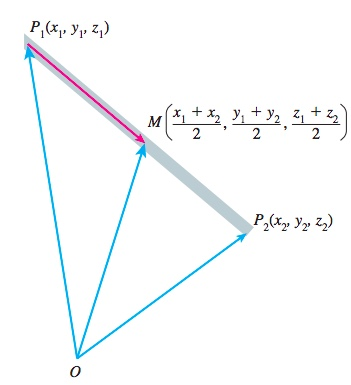
\includegraphics[scale=0.5]{figures_mvc/midpoint_formula}
\end{center}	
\end{pf}

\begin{exercise}
Find the midpoint of the segment joining $P_1=(3,-2,0)$ and $P_2(7,4,4)$.	
\end{exercise}

{\color{red} \flushleft {\bf Solution:}
The midpoint is the point
\begin{align*}
	\left(\frac{3+7}{2},\frac{-2+4}{2},\frac{0+4}{2}\right)=(5,1,2).
\end{align*}}

\subsection{The dot product}
Two nonzero vectors ${\bf u}$ and ${\bf v}$ positioned so that their initial points coincide determine an angle $\theta \in [0,\pi]$, which is the angle between the two vectors.
\begin{center}
	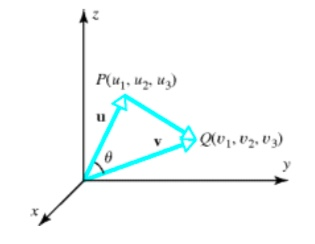
\includegraphics[scale=0.5]{figures_mvc/angle_uv}
\end{center}
Note that the information about $\theta$ is encoded in ${\bf u}-{\bf v}$, since if we fix the magnitudes of ${\bf u}$ and ${\bf v}$ and open the angle, then ${\bf u}-{\bf v}$ will also change. The fundamental relation satisfied by ${\bf u}, {\bf v}$ and $\theta$ is the law of cosines, which says that if ${\bf w}={\bf u}-{\bf v}$, then
\begin{equation}\label{eq:law_of_cosines}
	||{\bf w}||^2=||{\bf u}||^2+||{\bf v}||^2-2||{\bf u}|| \ ||{\bf v}||\cos \theta. 
\end{equation}
Let us make the following definition.
\begin{defn}[Dot product]
	The \ti{dot product} of two vectors ${\bf u}$ and ${\bf v}$ is defined by
	\begin{equation}\label{eq:dot_product_def}
		{\bf u}\cdot {\bf v}=||{\bf u}|| \ ||{\bf v}||\cos\theta.
	\end{equation} 
\end{defn}
The angle between two vectors ${\bf u}$ and ${\bf v}$ is then given by
\begin{equation}\label{eq:angle_uv}
	\theta=\cos^{-1}\left(\frac{{\bf u}\cdot {\bf v}}{||{\bf u}|| \ ||{\bf v}||}\right),
\end{equation}	
and we see that
\begin{itemize}
	\item $\theta$ is acute if ${\bf u} \cdot {\bf v} > 0$.
	\item $\theta$ is obtuse if ${\bf u} \cdot {\bf v} < 0$.
	\item $\theta$ is right if ${\bf u} \cdot {\bf v} = 0$.
\end{itemize}

Since the dot product takes as input two vectors and returns a scalar, it is also called the \ti{scalar product}. Note that from Eq. \eqref{eq:law_of_cosines}, we can write ${\bf u}\cdot {\bf v}$ in terms of magnitudes only, as 
\begin{equation}\label{eq:dot_product_magnitudes}
	{\bf u}\cdot {\bf v}=\frac{||{\bf u}||^2+||{\bf v}||^2-||{\bf u}-{\bf v}||^2}{2}.
\end{equation}
Note that this equation holds in \ti{all} coordinate systems. However, it takes a particularly simple form in Cartesian coordinates. Writing out the norm of each vector in terms of its components gives

\begin{align*}
	{\bf u}\cdot {\bf v}&=\frac{u_1^2+u_2^2+u_3^2+v_1^2+v_2^2+v_3^2-(u_1-v_1)^2-(u_2-v_2)^2-(u_3-v_3)^2}{2}
\end{align*}
Expanding the binomials and cancelling like terms, we find
\begin{equation}
	{\bf u}\cdot {\bf v}=u_1v_1+u_2v_2+u_3v_2.
\end{equation}

Note that we can write the norm of a vector using the dot product as 

\begin{equation}\label{eq:dot_product_norm}
	||{\bf u}||=\sqrt{{\bf u}\cdot {\bf u}}.
\end{equation}

\begin{exercise}
Compute the angle between the vectors ${\bf u}=(0,0,3)$ and ${\bf v}=(\sqrt{2},0,\sqrt{2})$.	
\end{exercise}

{\color{red} \flushleft {\bf Solution:} The angle between these vectors is
\begin{align*}
	\theta=\cos^{-1}\left(\frac{0(\sqrt{2}+0(0)+3(\sqrt{2}))}{3(2)}\right)=\cos^{-1}\left(\frac{1}{\sqrt{2}}\right)=\frac{\pi}{4}.
\end{align*}}

\begin{exercise}
	Find the angle between a diagonal of a cube and one of its edges.
\end{exercise}

{\color{red} \flushleft {\bf Solution:}
Let $s$ be the length of an edge and place the cube in the first octant so that one vertex is at the origin and two edges are along the $x$- and $y$-axes.
\begin{center}
	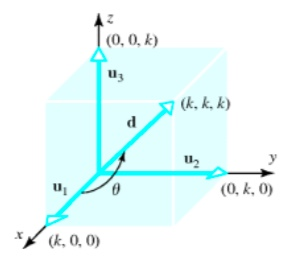
\includegraphics[scale=0.5]{figures_mvc/cube_coordinates}
\end{center}
If we let ${\bf u}_1=(s,0,0), {\bf u}_1=(0,s,0)$, and ${\bf u}_3=(0,0,s)$, then the vector
\begin{align*}
	{\bf d}=(s,s,s)={\bf u}_1+{\bf u}_2+{\bf u}_3
\end{align*}
is a diagonal of the cube. The angle between ${\bf d}$ and ${\bf u}_1$ is 
\begin{align*}
	\theta &=\cos^{-1}\left(\frac{{\bf u}_1 \cdot {\bf d}}{||{\bf u}_1 || \ || {\bf d}||}\right) \\
	&=\cos^{-1}\left(\frac{s^2}{(s)(\sqrt{3s^2})}\right)  \\
	&=\cos^{-1}\left(\frac{1}{\sqrt{3}}\right) \\
	&\approx 54.74^\circ.
\end{align*}
}

Let us now study the structural properties of the dot product.

\begin{prop}[Properties of the dot product]
	Let ${\bf a}, {\bf b}, {\bf c}, {\bf d}$ be vectors and $k$ any scalar. Then 
	\begin{enumerate}[(1)]
		\item ${\bf a}\cdot {\bf b}={\bf b} \cdot {\bf a}$
		\item $(k {\bf a})\cdot {\bf b}={\bf a}\cdot (k{\bf b})=k({\bf a}\cdot {\bf b})$
		\item ${\bf a}\cdot ({\bf b}+{\bf c})={\bf a}\cdot {\bf b}+{\bf a}\cdot {\bf c}$
		\item $({\bf a}+{\bf b})\cdot {\bf a}={\bf a}\cdot {\bf c}+{\bf b}\cdot {\bf c}$
		\item $({\bf a}+{\bf b})\cdot ({\bf c}+{\bf d})={\bf a}\cdot {\bf c}+{\bf a}\cdot {\bf d}+{\bf b}\cdot {\bf c}+{\bf b}\cdot {\bf d}$s
	\end{enumerate}
\end{prop}

\begin{pf}
Each of these can be proved by writing out the vectors in components. For example, to prove (1)
\begin{align*}
	{\bf a}\cdot {\bf b}&=a_1b_1+a_2b_2+a_3b_3 \\
	&=b_1a_1+b_2a_2+b_3a_3 \\
	&={\bf b}\cdot {\bf a}
\end{align*}
Properties (2)-(6) are proved similarly. Note that (5) follows from (3) and (4), but is included for emphasis since it is used frequently. 	
\end{pf}

\fixme{Add exercises using these properties.}

Note, however, the differences between the dot product and ordinary multiplication. For instance, one might ask, ``Is the dot product associative?". This question doesn't even make any sense for the dot product, as expressions such as ${\bf a}\cdot ({\bf b}\cdot {\bf c})$ are not defined, since ${\bf a}$ is a vector and $({\bf b}\cdot {\bf c})$ is a scalar, and one can only form the dot product between two vectors. 


Finally, the relationship between the dot product and the norm in Eq. \eqref{eq:dot_product_norm} implies two important inequalities:

\begin{prop}[Cauchy-Schwarz and triangle inequalities]
For any vectors ${\bf u}$ and ${\bf v}$, the following inequalities hold: \footnote{The first of these can be understood by taking ${\bf v}={\bf e}_1$. Since ${\bf u}\cdot {\bf e}_1=u_1$, the inequality becomes $|u_1| \leq ||{\bf u}||=\sqrt{u_1^2+u_2^2+u_3^2}$, which says the absolute value of any component of ${\bf u}$ is less than or equal to the length of ${\bf u}$. More generally, if $||{\bf v}|| \neq 0$ we can normalize both sides of the inequality by $||{\bf v}||$ to obtain $||{\bf u}\cdot \frac{{\bf v}}{||{\bf v}||}|| \leq ||{\bf u}||$, which says the \ti{projection of ${\bf u}$ along ${\bf v}$} (the length of the component of ${\bf u}$ along ${\bf v}$) is less than or equal to the length of ${\bf u}$. We will discuss projections   For the second, adding ${\bf u}+{\bf v}$ tip to tail, this inequality states the geometric fact that the length of any leg of a triangle is less than or equal to the sum of the other two.}
\begin{enumerate}[(a)]
	\item $||{\bf u}\cdot {\bf v}|| \leq ||{\bf u}|| \ ||{\bf v}||$ (Cauchy-Schwarz inequality)
		\item $||{\bf u}+{\bf v}||\leq ||{\bf u}|| + ||{\bf v}||$ (triangle inequality) 
\end{enumerate}
\end{prop}

\begin{pf}
	\begin{enumerate}[(a)]
			\item By (a), for any real number $\lambda$, we have $||{\bf u}-\lambda{\bf v}|| \geq 0$. Squaring both sides, we have
	\begin{align*}
		||{\bf u}-\lambda{\bf v}||^2&=({\bf u}-\lambda{\bf v})\cdot ({\bf u}-\lambda{\bf v}) \\
		&=\lambda^2{\bf v}\cdot {\bf v}-2\lambda {\bf u}\cdot {\bf v}+{\bf u}\cdot {\bf u} \\
		&=\lambda^2||{\bf v}||^2-2\lambda{\bf u}\cdot {\bf v}+||{\bf u}||^2 \geq 0
	\end{align*} 
In particular, if ${\bf v} \neq 0$, we can take $\lambda=\frac{{\bf u}\cdot {\bf v}}{||{\bf v}||^2}$, which gives
\begin{align*}
	||{\bf u}-\lambda{\bf v}||^2&=\frac{({\bf u}\cdot {\bf v})^2}{||{\bf v}||^4}||{\bf v}||^2-2\frac{{\bf u}\cdot {\bf v}}{||{\bf v}||^2}{\bf u}\cdot {\bf v}+||{\bf u}||^2 \\
	&=\frac{({\bf u}\cdot {\bf v})^2}{||{\bf v}||^2}-2\frac{({\bf u}\cdot {\bf v})^2}{||{\bf v}||^2}+||{\bf u}||^2 \\
	&=-\frac{({\bf u}\cdot {\bf v})^2}{||{\bf v}||^2}+||{\bf u}||^2 \geq 0\\
\end{align*}

and therefore
\begin{align*}
	({\bf u} \cdot {\bf v})^2 \leq ||{\bf u}||^2 \ ||{\bf v}||^2.
\end{align*}
The desired inequality then follows by taking the square root of both sides (which doesn't effect the inequality since both sides are nonnegative). If ${\bf v}=0$ the inequality also holds since both sides are zero, hence the inequality holds for all ${\bf u}$ and ${\bf v}$. \footnote{An alternative way to finish the proof is to note that if ${\bf u} \neq \lambda {\bf v}$, then $||{\bf u}-\lambda{\bf v}||^2=\lambda^2||{\bf v}||^2-2\lambda {\bf u}\cdot {\bf v}+||{\bf u}||^2>0$. This quadratic expression in $\lambda$ therefore has no real zeros, hence the discriminant $4({\bf u}\cdot {\bf v})^2-4||{\bf u}||^2||{\bf v}||^2>0$ which implies ${\bf u}\cdot {\bf v} \leq ||{\bf u}|| \ ||{\bf v}||$. If ${\bf u}=\lambda {\bf v}$, then one can easily check that the inequality still holds. Hence, the inequality is true for all ${\bf u}$ and ${\bf v}$.}
\item The triangle inequality follows from the Cauchy-Schwarz inequality:
\begin{align*}
	||{\bf u}+{\bf v}||^2&=({\bf u}+{\bf v})\cdot ({\bf u}+{\bf v}) \\
	&={\bf u} \cdot {\bf u}+{\bf v}\cdot {\bf v} +2{\bf u} \cdot {\bf v} \\
	&=||{\bf u}||^2+||{\bf v}||^2+2{\bf u} \cdot {\bf v} \\
	&\leq ||{\bf u}||^2+||{\bf v}||^2+||{\bf u}|| \ ||{\bf v}|| \hspace{0.25cm} (\text{ by Cauchy-Schwarz})\\
	&=(||{\bf u}||+||{\bf v}||)^2
\end{align*}
and the desired inequality follows by taking the square root of both sides.
	\end{enumerate}
\end{pf}


\subsection{Orthogonal vectors}
While writing vectors in component form has the advantage of facilitating many computations, this form seems to obscure geometric relations between vectors.
For instance, the two vectors
\begin{align*}
	{\bf u}&=(3,-2,1) \\
	{\bf v}&=(0,2,4).
\end{align*}
are orthogonal (perpendicular), but this does not seem obvious in the given form. We know from right triangle trigonometry that right angles are very special, so it would be nice to have a way to check if two vectors written in component form are perpendicular. Fortunately, the dot product gives us an easy way to determine this. 
\begin{prop}[Orthogonal vectors]\label{prop:orthogonal_vectors}
	Two nonzero vectors ${\bf a}$ and ${\bf b}$ are orthogonal if and only if ${\bf a}\cdot {\bf b}=0$.
\end{prop}

\begin{pf}
	The dot product of ${\bf a}$ and ${\bf b}$ is given by
\begin{align*}
	{\bf a}\cdot {\bf b}=||{\bf a}|| \ ||{\bf b}||\cos \theta.
\end{align*}	
If ${\bf a}$ and ${\bf b}$ are non-zero, then $||{\bf a}||$ and $||{\bf b}||$ are greater than zero, so ${\bf a}\cdot {\bf b}=0$ if and only if $\theta=\frac{\pi}{2}$, that is, if and only if ${\bf a}$ and ${\bf b}$ are orthogonal. 
\end{pf}

What if ${\bf b}={\bf 0}$? In this case, $\theta$ is not well-defined, since we have defined ${\bf 0}$ to be any vector with zero magnitude, independently of direction. For Proposition \ref{prop:orthogonal_vectors} to hold even if ${\bf a}$ or ${\bf b}$ are ${\bf 0}$, we simply define ${\bf a}\cdot {\bf b}=0$ if one of the vectors is the zero vector. With this definition, the zero vector is orthogonal to every vector, including itself.

\begin{example}
The two vectors in the example above	
\begin{align*}
	{\bf u}&=(3,-2,1) \\
	{\bf v}&=(0,2,4).
\end{align*}
are orthogonal since ${\bf u}\cdot {\bf v}=3(0)-2(2)+1(4)=-4+4=0$.
\end{example}

\begin{example}
	The standard unit vectors for $\mathbb{R}^3$ are mutually orthogonal. One can easily verify that 
	\begin{align*}
		{\bf e}_i \cdot {\bf e_j}=\delta_{ij}
	\end{align*}
where 
\begin{align*}
	\delta_{ij} \equiv \begin{cases}
		1 \text{ if } i=j, \\
		0 \text{ if } i \neq j
	\end{cases}
\end{align*}
is called the \ti{Kronecker delta symbol}.
\end{example}

These examples illustrate another difference between the dot product of two vectors and the ordinary product of two numbers. For two real numbers, if $ab=0$, then either $a=0$ or $b=0$. These examples clearly show that if ${\bf a}\cdot {\bf b}=0$, then it need not be true that either ${\bf a}=0$ or ${\bf b}=0$.
\subsection{Projection of a vector}
Let ${\bf a}$ be a nonzero vector, ${\bf \hat{a}}=\frac{{\bf a}}{||{\bf a}||}$ the unit vector obtained by normalizing ${\bf a}$, and ${\bf b}$ another vector. Then we have
\begin{align*}
	{\bf \hat{a}}\cdot {\bf b}=\frac{{\bf a}}{||{\bf a}||} \cdot {\bf b}=||{\bf b}||\cos \theta
\end{align*} 
is the component of ${\bf b}$ in the direction of ${\bf a}$. Multiplying by ${\bf \hat{a}}$, we get a vector parallel to ${\bf a}$ whose magnitude is the component of ${\bf b}$ along ${\bf a}$.

\begin{defn}[Orthogonal projection]
	The vector $\text{proj}_{\bf a}{\bf b}\equiv ({\bf \hat{a}}\cdot {\bf b}){\bf \hat{a}}=||{\bf b}||\cos \theta {\bf \hat{a}}$ is called the \ti{projection of ${\bf b}$ onto ${\bf a}$}.
\end{defn}
Geometrically, the projection of ${\bf b}=\overrightarrow{PQ}$ onto ${\bf a}=\overrightarrow{PS}$ is the vector $\overrightarrow{PR}$ determined by dropping a perpendicular from $Q$ to the line $PS$. \footnote{Note that by using the definitions of the dot product and the norm of ${\bf a}$, one may produce many equivalent expressions for $\text{proj}_{\bf a}{\bf b}$:
\begin{align*}
	\text{proj}_{\bf a}{\bf b}&=(||{\bf b}||\cos \theta){\bf \hat{a}} \\
	&=({\bf \hat{a}}\cdot {\bf b}){\bf \hat{a}} \\
	&=\left(\frac{{\bf a}\cdot {\bf b}}{||{\bf a}||}\right)\frac{{\bf a}}{||{\bf a}||} \\
	&=\left(\frac{{\bf b}\cdot {\bf a}}{{\bf a}\cdot {\bf a}}\right){\bf a}
\end{align*}
The first of these is perhaps the easiest to remember, as it makes most transparent the relation to elementary right triangle trigonometry.}

\begin{center}
	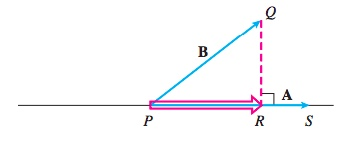
\includegraphics[scale=0.5]{figures_mvc/vector_projection_def}
\end{center}
Physically, if ${\bf b}$ represents a force, then $\text{proj}_{\bf a}{\bf b}$ is the effective force in the ${\bf a}$ direction.

\begin{center}
	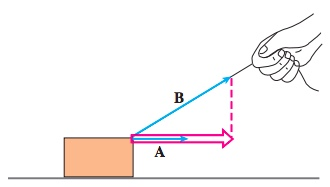
\includegraphics[scale=0.5]{figures_mvc/effective_force_box}
\end{center}	

It is often desirable to express a vector ${\bf b}$ as a sum of two orthogonal vectors. For instance, in mechanics we frequently decompose forces in this way so that we may treat a two-dimensional problem as two one-dimensional problems. We can easily express a vector ${\bf b}$ as such a sum of two vectors, one parallel to some nonzero vector ${\bf a}$ and one orthogonal to ${\bf a}$, in terms of the projection of ${\bf b}$ along ${\bf a}$:
\begin{equation}
\begin{split}
	{\bf b}&={\bf b}_{\parallel}+{\bf b}_{\perp} \\
	&=\text{proj}_{\bf a}{\bf b}+({\bf b}-\text{proj}_{\bf a}{\bf b}).
\end{split}
\end{equation}

\begin{center}
	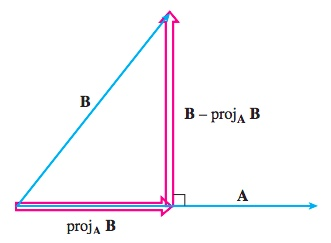
\includegraphics[scale=0.5]{figures_mvc/sum_of_orthogonal_vectors}
\end{center}

\begin{exercise}
	Express ${\bf b}=2{\bf e}_1+{\bf e}_2-3{\bf e}_3$ as the sum of a vector parallel to ${\bf a}=3{\bf e}_1-{\bf e}_2$ and a vector orthogonal to ${\bf a}$.
\end{exercise}

{\color{red} \flushleft {\bf Solution:}
Since ${\bf \hat{a}}\equiv \frac{{\bf a}}{||{\bf a}||}=\frac{3{\bf e}_1-{\bf e}_2}{\sqrt{10}}$, we can write ${\bf b}={\bf b}_{\parallel}+{\bf b}_{\perp}$ with  
\begin{align*}
	{\bf b}_{\parallel}&=({\bf \hat{a}}\cdot {\bf b}){\bf {\hat{a}}}=\frac{1}{2}(3{\bf e}_1-{\bf e}_2)=\frac{1}{2}{\bf a} \\
	{\bf b}_{\perp}&={\bf b}-{\bf b}_{\parallel}=\frac{1}{2}{\bf e}_1+\frac{3}{2}{\bf e}_2-3{\bf e}_3.
\end{align*}}

\begin{example}[Distance between a point and a line]
We can use orthogonal projections to compute the perpendicular distance between a line $\ell$ and any point $P$ not on the line. Let $P_0$ be any point on $\ell$ and ${\bf \hat{v}}$ a unit vector along $\ell$. The perpendicular distance $d$ from $P$ to $\ell$ is then
\begin{align*}
	d=||\overrightarrow{P_0P}-\text{Proj}_{{\bf \hat{v}}}\overrightarrow{P_0P}||.
\end{align*}	
\end{example}

\begin{center}
	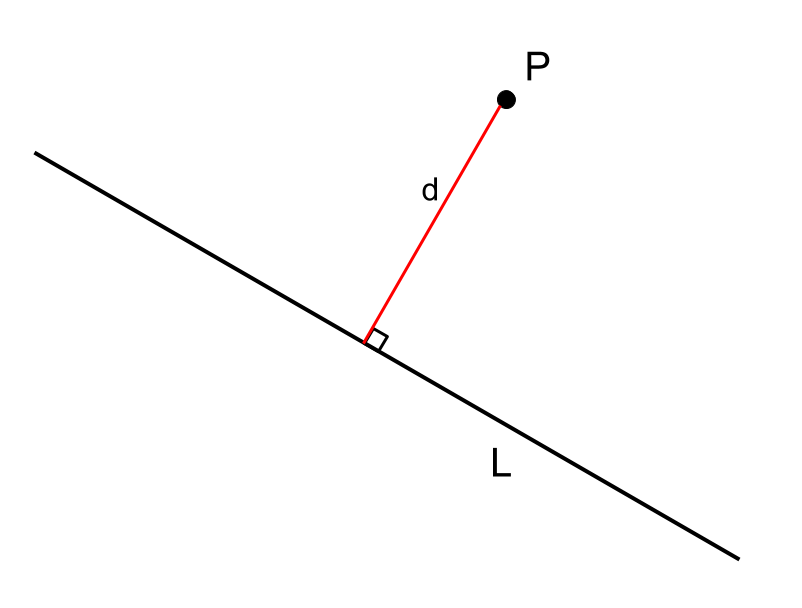
\includegraphics[scale=0.3]{figures_mvc/distance_between_line_and_point}
\end{center}

\begin{exercise}
Find the distance from the point $P=(2,1,-1)$ to the line $(x,y,z)=(2-t,t,1+t)$.	
\end{exercise}

{\color{red} \flushleft {\bf Solution:}
We can find a point on the line by plugging in any number for $t$, such as $t=0$, which gives us the point $P_0=(2,0,1)$. To get a vector along the line, we need another point on the line. Plugging in $t=1$, we have $Q_0=(1,1,2)$. A vector along the line is $\overrightarrow{P_0Q_0}=(1,-1,-1)$ and normalizing gives ${\bf \hat{v}}=\frac{1}{\sqrt{3}}(1,-1,-1)$. The distance from $P$ to the line is the length of the component of $\overrightarrow{P_0P}=(0,1,-2)$ which is orthogonal to ${\bf \hat{v}}=\frac{1}{\sqrt{3}}(1,-1,-1)$. This is given by
\begin{align*}
	||\overrightarrow{P_0P}-\text{proj}_{\bf \hat{v}}\overrightarrow{P_0P}||&=||\overrightarrow{P_0P}-(\overrightarrow{P_0P} \cdot {\bf v}){\bf v}|| \\
	&=||(0,1,-2)-\frac{1}{3}(1,-1,-1)|| \\
	&=||(-\frac{1}{3},\frac{4}{3}, -\frac{5}{3})|| \\
	&=\sqrt{(-\frac{1}{3})^2+(\frac{4}{3})^2+(-\frac{5}{3})^2} \\
	&=\frac{\sqrt{42}}{3}.
\end{align*}}


\subsection{The cross product}
There is another vector product which is important in physics, known as the \ti{cross product}. Unlike the dot product, which took two vectors and returned a \ti{scalar}, the cross product takes two vectors and returns another \ti{vector}.

The physical motivation for the cross product is that of \ti{torque}, which is a force that causes a rotation. Suppose we wish to tighten a bolt using a wrench. Applying a force ${\bf F}$ to the handle of the wrench produces a torque which acts along the axis of the bolt to drive the bolt forward. The magnitude of the torque depends on three things:
\begin{enumerate}
	\item The magnitude of ${\bf F}$. That is, how hard we push.
	\item How far out on the handle we apply the force. We denote the vector from the bolt to the point on the handle where the force is applied by ${\bf r}$. This vector is called the \ti{lever arm}. So, the magnitude of the torque also depends on the magnitude of the lever arm.
	\item Finally, the magnitude of the torque depends on the angle with respect to the axis of the handle at which the force is applied. \footnote{The angle we refer to here will be taken to be the \ti{smaller} of the two angles between the force vector and the lever arm.} The torque is zero when this angle is zero (since a force directed \ti{along} the axis of the wrench causes no rotation) and the torque is maximized then the force is perpendicular to the axis of the wrench.
\end{enumerate}
Denoting the torque by $\vec{\tau}$, one observes that 
\begin{equation}\label{eq:magnitude_of_torque}
	||\vec{\tau}||=||{\bf r}||\ ||{\bf F}||\ \sin \theta
\end{equation}
where, again, $\theta$ is the \ti{smaller} of the two angles between ${\bf r}$ and ${\bf F}$.
\begin{center}
	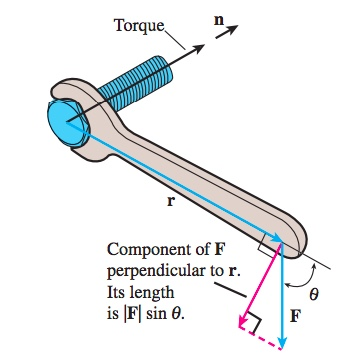
\includegraphics[scale=0.5]{figures_mvc/torque_wrench}
\end{center}
This gives the magnitude of $\vec{\tau}$. Notice that if we take the fingers of our \ti{right} hand and point then along the direction of ${\bf r}$ and then curl them toward ${\bf F}$ through the angle $\theta$ between ${\bf r}$ and ${\bf F}$ (arranged so that their initial points coincide), then our thumb points in the direction of $\vec{\tau}$. This is called the \ti{right-hand rule}. Letting ${\bf n}$ be a unit vector in the direction of $\vec{\tau}$ we have therefore found
\begin{equation}
	\vec{\tau}=||{\bf r}|| \ ||{\bf F}|| \ \sin \theta{\bf n}.
\end{equation}

\begin{example}
The magnitude of the torque exerted by the force ${\bf F}$ about the pivot point $P$ below 

\begin{center}
	\includegraphics[scale=0.5]{figures_mvc/torque_example}
\end{center}

is 
\begin{align*}
	||\vec{\tau}||=||\overrightarrow{PQ}|| \ ||{\bf F}|| \sin \theta = (3)(20)\sin 70^\circ \approx 56.4 \text{ ft-lb}.
\end{align*}
By the right hand rule, the torque is perpendicular to the plane  containing ${\bf r}$ and ${\bf F}$, and pointing \ti{out} of the page (rather than \ti{into} the page).
\end{example}


\begin{defn}[Cross product]
The \ti{cross product} of two nonzero vectors ${\bf a}$ and ${\bf b}$ is the vector
\begin{equation}
	{\bf a} \times {\bf b}=||{\bf a}|| \ ||{\bf b}|| \ \sin \theta{\bf n}
\end{equation}
where $\theta$ is the angle between ${\bf a}$ and ${\bf b}$ and ${\bf n}$ is a unit vector in the direction determined by the right-hand rule (that is, upon directing the fingers of ones right hand in the direction of ${\bf a}$ and curling them toward ${\bf b}$ through $\theta$, then ones thumb points in the direction of ${\bf n}$ and therefore $\overrightarrow{\tau}$). 

If either ${\bf a}$ or ${\bf b}$ is the zero vector, then we define ${\bf a} \times {\bf b}$ to be ${\bf 0}$.
\end{defn}

If ${\bf a}$ and ${\bf b}$ are both nonzero and if $\theta \neq 0$, then ${\bf a}$ and ${\bf b}$ define a plane, and ${\bf n}$ is perpendicular to this plane. The sense of ${\bf n}$ is the one determined by the right hand rule. 
\begin{center}
	\includegraphics[scale=0.5]{figures_mvc/cross_product}
\end{center}
Thus, 
\begin{center}
	\ti{The cross product ${\bf a} \times {\bf b}$ is a vector perpendicular to both ${\bf a}$ and ${\bf b}$}.
\end{center}

Note that if $\theta=0$ or $\pi$ (that is, if ${\bf a}$ and ${\bf b}$ are parallel, which means they don't determine a plane), then ${\bf a} \times {\bf b}=0$ . Conversely, if ${\bf a}$ and ${\bf b}$ are both non-zero, then we see from the definition that ${\bf a} \times {\bf b}=0$ only if ${\bf a}$ and ${\bf b}$ are parallel. Hence, we have proved the following proposition.

\begin{prop}[Parallel vectors]
	Two nonzero vectors ${\bf a}$ and ${\bf b}$ are parallel if and only if 
	\begin{align*}
		{\bf a} \times {\bf b}=0.
	\end{align*}
\end{prop}

Note that, geometrically, the magnitude of the cross product $||{\bf a} \times {\bf b}||=||{\bf a}|| \ ||{\bf b}||\sin\theta$ is the area of the parallelogram with adjacent sides ${\bf a}$ and ${\bf b}$:
\begin{center}
	\includegraphics[scale=0.5]{figures_mvc/cross_product_area_of_parallelogram}
\end{center}

Let us now look at the properties of the cross product. Despite its usefulness in physics, it turns out to preserve almost none of the properties of ordinary numerical multiplication. In particular, the cross product is neither commutative nor associative:


\begin{enumerate}[(1)]
	\item ${\bf a} \times {\bf b} \neq {\bf b}  \times {\bf a}$
	\item ${\bf a} \times ({\bf b} \times {\bf c}) \neq ({\bf a} \times {\bf b}) \times {\bf c}$
\end{enumerate}	

Regarding the first of these, if we reverse ${\bf a}$ and ${\bf b}$ in the definition, the only difference is that we rotate ${\bf b}$ into ${\bf a}$ rather than ${\bf a}$ into ${\bf b}$, so the right and rule gives
\begin{equation}
	{\bf a} \times {\bf b}=-{\bf b} \times {\bf a}.
\end{equation}
One the other hand, for the second of these, not only are the magnitudes of ${\bf a} \times ({\bf b} \times {\bf c})$ and $({\bf a} \times {\bf b}) \times {\bf c}$ not necessarily equal, these vectors do not even have to lie in the same plane! \footnote{Applying the definition of each cross product, one finds that ${\bf a} \times ({\bf b} \times {\bf c})$ is parallel to the plane determined by ${\bf b}$ and ${\bf c}$, while $({\bf a} \times {\bf b}) \times {\bf c}$ is parallel to the plane determined by ${\bf a}$ and ${\bf b}$. In particular, there is no reason why the ${\bf a}{\bf b}$-plane and the ${\bf b}{\bf c}$-plane should be the same, since three vectors don't have to lie in the same plane.}

However, vector and scalar distributive laws \ti{do} hold for the cross product:
\begin{prop}[Distributive properties of the cross product]
	\begin{enumerate}[(1)]\hspace{10cm}
	\item $(r{\bf a}) \times (s{\bf b})=(rs)({\bf a} \times {\bf b})$,
	\item ${\bf a} \times ({\bf b} + {\bf c})={\bf a} \times {\bf b}+{\bf a} \times {\bf c}$.
\end{enumerate}
\end{prop}

\begin{pf}
\begin{enumerate}[(1)]\hspace{10cm}
	\item We can verify this formula by applying the definition of the cross product to both sides of the equation:
	\begin{align*}
		||(r{\bf a}) \times (s{\bf b})||&=||(r{\bf a}) || \ ||(s{\bf b})||\sin \theta  \\&=|r| \ |s | \ ||{\bf a} || \ ||{\bf b} || \sin \theta \\
		&=|rs| \ ||{\bf a} || \ ||{\bf b} || \sin \theta \\
		&=||(rs)({\bf a}\times {\bf b})||
	\end{align*}
where we have used the fact that the angle between ${\bf a}$ and ${\bf b}$ is the same as the angle between $r{\bf a}$ and $s{\bf b}$.
	\item To derive this formula, we construct ${\bf a} \times {\bf b}$ in a new way. Draw ${\bf a}$ and ${\bf b}$ from the common point $O$ and construct a plane perpendicular to ${\bf a}$ at $O$.
\begin{center}
	\includegraphics[scale=0.5]{figures_mvc/distributivity_of_the_cross_product_1}
\end{center}
We then project ${\bf b}$ orthogonally onto $M$, yielding a vector ${\bf b}'$ with length $||{\bf b}||\sin \theta$. Finally, we rotate ${\bf b}'$ $90^\circ$ about ${\bf a}$ in the positive sense to produce a vector ${\bf b}''$, and then multiply ${\bf b}''$ by the length of ${\bf a}$. The resulting vector $||{\bf a}||{\bf b}''$ is equal to ${\bf a} \times {\bf b}$ since it has the same direction as ${\bf a} \times {\bf b}$ by construction and 
\begin{align*}
	||{\bf a}|| \ ||{\bf b}''||&=||{\bf a}|| \ ||{\bf b}'|| \ \text{ (since ${\bf b}''$ and ${\bf b}'$ are related by a rotation)} \\
	&=||{\bf a}|| \ ||{\bf b}||\sin\theta \ \text{ (since ${\bf b}'$ is the projection of ${\bf b}$ onto $M$)} \\
	&=||{\bf a} \times {\bf b}||. 
\end{align*}
Now each of these three operations, namely,
\begin{enumerate}
\item projection onto $M$,
\item rotation about ${\bf a}$ through $90^\circ$, 
\item multiplication by the scalar $||{\bf a}||$,
\end{enumerate}
when applied to a triangle whose plane is not parallel to ${\bf a}$, will produce another triangle. \footnote{If the triangle is in a plane parallel to ${\bf a}$ then projection onto $M$ will give a line segment, not a triangle.} If we start with a triangle whose sides are ${\bf b}, {\bf c},$ and ${\bf b}+{\bf c}$ and apply these three steps, we successively obtain
\begin{center}
	\includegraphics[scale=0.5]{figures_mvc/distributivity_of_the_cross_product_2}
\end{center}
\begin{enumerate}
\item a triangle whose sides are ${\bf b}', {\bf c}',$ and $({\bf b}+{\bf c})'$ satisfying the vector equation
	\begin{align*}
		{\bf b}'+{\bf c}'=({\bf b}+{\bf c})';
	\end{align*}
\item a triangle whose sides are ${\bf b}'', {\bf c}'',$ and $({\bf b}+{\bf c})''$ satisfying the vector equation
	\begin{align*}
		{\bf b}''+{\bf c}''=({\bf b}+{\bf c})'';
	\end{align*}
	and, finally,
\item a triangle whose sides are $||{\bf a}||{\bf b}'',$ $||{\bf a}||{\bf c}''$, and $||{\bf a}({\bf b}+{\bf c})''$ satisfying the vector equation
	\begin{equation}\label{eq:distributive_cross_product}
		||{\bf a}||{\bf b}''+||{\bf a}||{\bf c}''=||{\bf a}||({\bf b}+{\bf c})''.
	\end{equation}
\end{enumerate}
But we have shown above that $||{\bf a}||{\bf b}''={\bf a} \times {\bf b}$, $||{\bf a}||{\bf c}''={\bf a} \times {\bf c}$, and $||{\bf a}||({\bf b}+{\bf c})''={\bf a} \times ({\bf b}+{\bf c})$,
and therefore Eq. \eqref{eq:distributive_cross_product} is equivalent to 
\begin{align*}
	{\bf a} \times {\bf b}+{\bf a} \times {\bf c}={\bf a} \times ({\bf b} + {\bf c}),
\end{align*}
which is the property we wanted to establish.
\end{enumerate}	
\end{pf}

The cross product takes a useful form in  Cartesian coordinates. Let us first work out the various cross products of pairs of the unit vectors ${\bf e}_1, {\bf e}_2, {\bf e}_3$. Applying the definitions of the cross product and the ${\bf e}_i$s, we find 
\begin{align*}
	{\bf e}_i \times {\bf e}_j=\epsilon_{ijk}{\bf e}_k
\end{align*}
for $i,j,k \in \{1,2,3\}$, where
\begin{align*}
	\epsilon_{ijk}=\begin{cases}
		1, \text{ if $(ijk)$ is an even permutation of $(123)$} \\
		-1, \text{ if $(ijk)$ is an odd permutation of $(123)$} \\
		0, \text{ otherwise}
	\end{cases}
\end{align*}
Now let
\begin{align*}
	{\bf a}&=a_1{\bf e}_1+a_2{\bf e}_2+a_3{\bf e}_3 \\
	{\bf b}&=b_1{\bf e}_1+b_2{\bf e}_2+b_3{\bf e}_3 \\
\end{align*} 
We compute ${\bf a} \times {\bf b}$ using the distributive property above and then use the cross products of the ${\bf e}_i$s worked out above to simplify the 9 terms, ending up with \footnote{Those who have previously studied determinants can easily verify that this formula may be written as  
\begin{align*}
	{\bf a} \times {\bf b}=\begin{vmatrix}
		{\bf e}_1 & {\bf e}_2 & {\bf e}_3 \\
		a_1 & a_2 & a_3 \\
		b_1 & b_2 & b_3
	\end{vmatrix},
\end{align*} which is a useful mnemonic to remember the formula in Eq. \eqref{eq:a_cross_b}. We will study determinants in detail in a later unit.}
\begin{equation}\label{eq:a_cross_b}
	{\bf a} \times {\bf b}=(a_2b_3-a_3b_2){\bf e}_1-(a_1b_3-a_3b_1){\bf e}_2+(a_1b_2-a_2b_1){\bf e}_3.
\end{equation}
\fixme{Discuss even odd permutations of $(123)$ and how to remember the signs.}

\begin{exercise}
Compute ${\bf a} \times {\bf b}$ and ${\bf b} \times {\bf a}$ if ${\bf a}=(2,1,1)$ and ${\bf b}=(-4,3,1)$.	
\end{exercise}

{\color{red} \flushleft {\bf Solution:}
\begin{align*}
	{\bf a} \times {\bf b}&=\begin{vmatrix}
		{\bf e}_1 & {\bf e}_2 & {\bf e}_3 \\
		2 & 1 & 1 \\
		-4 & 3 & 1
	\end{vmatrix}
	=(-2,-6,10). \\
	{\bf b} \times {\bf a}&=-{\bf a} \times {\bf b}=(2,6,-10).
\end{align*}
}

\begin{exercise}
Find a vector perpendicular to the plane of $P(1,-1,0), Q(2,1,-1),$ and $R(-1,1,2)$.	
\end{exercise}

{\color{red} \flushleft {\bf Solution:}
Any three lines lie in a plane. We can construct two vectors in this plane:
\begin{align*}
	\overrightarrow{PQ}=(2-1,1-(-1),-1-0)=(1,2-1), \\
	\overrightarrow{PR}=(-1-1,1-(-1),2-0)=(-2,2,2). \\
\end{align*}
A vector perpendicular to this plane is then given by
\begin{align*}
	\overrightarrow{PQ} \times \overrightarrow{PR} =\begin{vmatrix}
		{\bf e}_1 & {\bf e}_2 & {\bf e}_3 \\
		1 & 2 & -1 \\ -2 & 2 & 2
	\end{vmatrix} = (6,0,6).
\end{align*}}

\begin{exercise}
	Find the area of the triangle with vertices $P(1,-1,0), Q(2,1,-1),$ and $R(-1,1,2)$.
\end{exercise}
{\color{red} \flushleft {\bf Solution:}
The area of the parallelogram determined by $P,Q,$ and $R$ is 
\begin{align*}
	||\overrightarrow{PQ} \times \overrightarrow{PR}||=||(6,0,6)||=6\sqrt{2}.
\end{align*}
The triangles area is half of this, or $3\sqrt{2}$.
\begin{center}
	\includegraphics[scale=0.5]{figures_mvc/triangle_area_cross_product}
\end{center}
}

\begin{exercise}
Find a unit vector perpendicular to the plane containing $P(1,-1,0), Q(2,1,-1),$ and $R(-1,1,2)$.	
\end{exercise}

{\color{red} \flushleft {\bf Solution:}
A unit vector perpendicular to the plane is given by
\begin{align*}
	{\bf n}=\frac{\overrightarrow{PQ} \times \overrightarrow{PR}}{||\overrightarrow{PQ} \times \overrightarrow{PR}||}=\frac{(6,0,6)}{6\sqrt{2}}=(1/\sqrt{2},0,1/\sqrt{2}).
\end{align*}}

\subsection{The triple scalar product}
Since ${\bf a} \times {\bf b}$ is a vector, note that the product $({\bf a} \times {\bf b}) \cdot {\bf c}$ is defined.

\begin{defn}[Triple scalar product]
	For any vectors ${\bf a}, {\bf b},$ and ${\bf c}$, the \ti{triple scalar product} is defined by
	\begin{align*}
		({\bf a} \times {\bf b}) \cdot {{\bf c}}=||{\bf a} \times {\bf b}|| \ ||{\bf c}|| \cos \theta
	\end{align*}
where $\theta$ is the angle between ${\bf a} \times {\bf b}$ and ${\bf c}$.
\end{defn}

Geometrically, the magnitude of ${\bf a} \times {\bf b} \cdot {{\bf c}}$ is the volume of the parallelepiped whose with adjacent sides ${\bf a}, {\bf b}$, and ${\bf c}$, the number $||{\bf a} \times {\bf b}||$ being the area of the base parallelogram and $||{\bf c}||\cos \theta$ the height of the parallelepiped.
\begin{center}
	\includegraphics[scale=0.5]{figures_mvc/triple_scalar_product_parallelepiped}
\end{center}
For this reason, the triple scalar product is also called the \ti{box product} of ${\bf a}, {\bf b},$ and ${\bf c}$.

Computing the triple scalar product in Cartesian coordinates, one can verify that 
\begin{equation}\label{eq:triple_scalar_product_formula}
\begin{split}
		({\bf a} \times {\bf b}) \cdot {{\bf c}}&=a_1(b_2c_3-c_3b_2)-a_2(b_1c_3-b_3c_1)+a_3(b_1c_2-c_1b_2)	 \\
		&=\begin{vmatrix}
		a_1 & a_2 & a_3 \\
		b_1 & b_2 & b_3 \\
		c_1 & c_2 & c_3  
	\end{vmatrix}. \\
\end{split}
\end{equation}

\begin{prop}[Cyclic symmetry of triple scalar product]\label{eq:cyclic_symmetry_of_triple_scalar_product}
For any three vectors ${\bf a}, {\bf b},$ and ${\bf c}$, the triple scalar product satisfies
\begin{align*}
	({\bf a} \times {\bf b}) \cdot {\bf c}=({\bf b} \times {\bf c}) \cdot {\bf a}=({\bf c} \times {\bf a}) \cdot {\bf b}.
\end{align*}	
\end{prop}

\begin{pf}
This is straightforward to verify from Eq. \eqref{eq:triple_scalar_product_formula}. For those who know about determinants, the determinant is unchanged under cyclic permutations of the rows.
\end{pf}

\begin{cor}[Interchange of dot and cross product in triple scalar product]
For any three vectors ${\bf a}, {\bf b},$ and ${\bf c}$, the triple scalar product satisfies
\begin{align*}
	({\bf a} \times {\bf b}) \cdot {\bf c}={\bf a}\cdot ({\bf b} \times {\bf c})
\end{align*}	
\end{cor}

\begin{pf}
This follows from Proposition \ref{eq:cyclic_symmetry_of_triple_scalar_product} along with commutativity of the dot product.	
\end{pf}

\begin{exercise}
Find the volume of the parallelepiped with adjacent sides ${\bf a}=(1,2,-1), {\bf b}=(-2,0,3)$, and ${\bf c}=(0,7,-4)$.	
\end{exercise}

{\color{red} \flushleft {\bf Solution:}
This is given by
\begin{align*}
	||{\bf a} \cdot ({\bf b} \times {\bf c})||=\vert \begin{vmatrix}
		1 & 2 & -1 \\ -2 & 0 & 3 \\ 0 & 7 & -4
	\end{vmatrix} \vert = \vert -23 \vert = 23.
\end{align*}}

\subsection{Equations of lines and planes}
\subsubsection{Lines in space}
The coordinate systems of analytic geometry allow us to consider geometric objects such as lines and planes in terms of vectors. These geometric ideas will give us valuable intuition later on in the course when we take a more abstract point of view toward vectors.

First let us recall that any two points define a line. Equivalently, we can also determine a line if we know one point on the line and the slope of the line. 

Let us now work in Cartesian coordinates. Suppose $L$ is a line passing through a point $P_0(x_0,y_0,z_0)$ and parallel to a vector ${\bf v}=v_1{\bf e}_1+v_2{\bf e}_2+v_3{\bf e}_3$. Now let $P(x,y,z)$ be any point in space. In which case will $P(x,y,z)$ to be on the line? This will be the case if the vector $\overrightarrow{P_0P}$ is parallel to ${\bf v}$, that is, if $\overrightarrow{P_0P}$ is a scalar multiple of ${\bf v}$. Therefore,
\begin{defn}[Vector equation for a line]
	The line through $P_0(x_0,y_0,z_0)$ and parallel of ${\bf v}$ is the set of all points $P(x,y,z)$ such that $\overrightarrow{P_0P}=t{\bf v}$, with $-\infty < t < \infty$. This equation is called the \ti{vector equation} of the line.
\end{defn}
In terms of Cartesian coordinates, the vector equation for the line becomes
\begin{align*}
	(x-x_0){\bf e}_1+(y-y_0){\bf e}_2+(z-z_0){\bf e}_3&=t(v_1{\bf e}_1+v_2{\bf e}_2+v_3{\bf e}_3) \\
	&=tv_1{\bf e}_1+tv_2{\bf e}_2+tv_3{\bf e}_3
\end{align*}
which implies
\begin{align*}
	(x-x_0-tv_1){\bf e}_1+(y-y_0-tv_2){\bf e}_2+(z-z_0-tv_3){\bf e}_3={\bf 0}
\end{align*}
and hence
\begin{equation}\label{eq:parametric_equations_line}
	x=x_0+tv_1, \hspace{0.25cm} y=y_0+tv_2, \hspace{0.25cm} z=z_0+tv_3.
\end{equation}
Thus, the vector equation of the line is equivalent to the three scalar equations in Eq. \eqref{eq:parametric_equations_line}, each of which is the usual equation for a line with slope $v_i$ in one variable $t$.

\begin{defn}[Parametric equations for a line]
	The standard parametrization of the line through $P_0(x_0,y_0,z_0)$ and parallel to ${\bf v}=v_1{\bf e}_1+v_2{\bf e}_2+v_3{\bf e}_3$ is given by
	\begin{align*}
		x=x_0+tv_1, \hspace{0.25cm} y=y_0+tv_2, \hspace{0.25cm} z=z_0+tv_3.
	\end{align*}
	These equations are called the (standard) \ti{parametric equations} for the line.
\end{defn}

\begin{exercise}
Find the parametric equations for the line through $(-2,0,4)$ and parallel to ${\bf v}=2{\bf e}_1+4{\bf e}_2-2{\bf e}_3$.	
\end{exercise}

{\color{red} \flushleft {\bf Solution:}
Plugging into Eq. \eqref{eq:parametric_equations_line} gives
\begin{align*}
	x=-2+2t, \hspace{0.25cm} y=4t, \hspace{0.25cm} z=4-2t.
\end{align*}}
\begin{center}
	\includegraphics[scale=0.5]{figures_mvc/parametrized_line_example_1}
\end{center}

\begin{example}
	Find parametric equations for the line through $P(-3,2,-3)$ and $Q(1,-1,4)$.
\end{example}

{\color{red} \flushleft {\bf Solution:}
The vector from $P$ to $Q$ is 
\begin{align*}
	\overrightarrow{PQ}&=(1-(-3), -1-2, 4-(-3)) \\
	&=(4,-3,7).
\end{align*}
We take this vector to be our ``${\bf v}$". The point $P_0$ could be either $P$ or $Q$. Arbitrarily choosing it to be $Q$, Eq. \eqref{eq:parametric_equations_line} gives
\begin{align*}
	x=1+4t, \hspace{0.25cm} y=-1-3t, \hspace{0.25cm} z=4+7t.
\end{align*}}

\begin{exercise}
Parametrize the line segment joining the points $P(-3,2,-3)$ and $Q(1,-1,4)$.	
\end{exercise}
{\color{red} \flushleft {\bf Solution:}
We have seen in the previous exercise that the  parametric equations 
\begin{align*}
	x=1+4t, \hspace{0.25cm} y=-1-3t, \hspace{0.25cm} z=4+7t.
\end{align*}
describe an infinite line containing $P$ and $Q$ when we take $-\infty < t < \infty$. To describe the line segment joining $P$ and $Q$, we simply restrict the domain of $t$. We see that the line passes through $P$ at $t=-1$ and $Q=0$. So the line segment joining $P$ and $Q$ is given by 

\begin{align*}
	x=1+4t, \hspace{0.25cm} y=-1-3t, \hspace{0.25cm} z=4+7t.
\end{align*}

with $-1 < t < 0$.}

\subsubsection{Planes in space}
Whereas a line is determined by any two points, a plane is determined by any \ti{three} non-collinear points. Similar to a line, which was equivalently determined by a single point and a slope, a plane can also be determined by a single point and a ``slope". The direction of the plane is determined by a normal vector ${\bf n}=n_1{\bf e}_1+n_2{\bf e}_2+n_3{\bf e}_3$. 

Let us now repeat the question we asked before: given a point $P_0(x_0,y_0,z_0)$ on the plane and a vector ${\bf n}$ normal to the plane, what is the condition for an arbitrary point in space $P(x,y,z)$ to lie on the plane? If $P$ lies in the plane, the $\overrightarrow{P_0P}$ is a vector lying in the plane. Then, since ${\bf n}$ is normal to the plane, we must have that ${\bf n} \cdot \overrightarrow{P_0P}=0$.

\begin{center}
	\includegraphics[scale=0.5]{figures_mvc/vector_equation_of_a_plane}
\end{center}

\begin{defn}[Vector equation for a plane]
	The \ti{vector equation} of the plane through $P_0(x_0,y_0,z_0)$ and normal to ${\bf n}=n_1{\bf e}_1+n_2{\bf e}_2+n_3{\bf e}_3$ is given by
	\begin{equation}
		{\bf n} \cdot \overrightarrow{P_0P}=0.
	\end{equation}
\end{defn}

As before, we can expand this equation in Cartesian coordinates to obtain

\begin{defn}[The component equation of a plane]
	The component equation of a plane through $P_0(x_0,y_0,z_0)$ and normal to ${\bf n}=n_1{\bf e}_1+n_2{\bf e}_2+n_3{\bf e}_3$ is given by
	\begin{equation}
		n_1(x-x_0)+n_2(y-y_0)+n_3(z-z_0)=0.
	\end{equation}
	This can be simplified to 
	\begin{equation}
		n_1x+n_2y+n_3z=c
	\end{equation}
	where $c=n_1x_0+n_2y_0+n_3z_0$.
\end{defn}

\begin{exercise}
Find an equation for the plane through $P_0(-3,0,7)$ perpendicular to ${\bf n}=(5,2,-1)$.	
\end{exercise}

{\color{red} \flushleft {\bf Solution:}
The component equation is 
\begin{align*}
	5(x-(-3))+2(y-0)+(-1)(z-7)=0,
\end{align*}
Simplifying, we obtain
\begin{align*}
	5x+15+2y-z+7&=0 \\
	5x+2y-z&=-22.
\end{align*}}

\begin{exercise}
Find the point where the line 
\begin{align*}
	x=\frac{8}{3}+2t, \hspace{0.25cm} y=2t, \hspace{0.25cm} z=1+t
\end{align*}	
intersects the plane $3x+2y+6z=6$.
\end{exercise}

{\color{red} \flushleft {\bf Solution:}
The point $(\frac{8}{3}+2t, 2t, 1+t)$ lies in the plane if its coordinates satisfy the equation of the plane; that is, if
\begin{align*}
	3(\frac{8}{3}+2t)+2(-2t)+6(1+t)=6
\end{align*}
This has a solution at $t=-1$, so the point of intersection is 
\begin{align*}
	(x,y,z)\vert_{t=-1}=(\frac{2}{3},2,0).
\end{align*}}

\begin{exercise}
\begin{enumerate}[(a)]
	\item Find a vector parallel to the line of intersection of the planes $3x-6y-2z=15$ and $2x+y-2z=5$.	
	\item Find parametric equations for the line in which these planes intersect.
\end{enumerate}
\end{exercise}

\fixme{Add solution.}

\begin{example}[Distance between a point and a plane]
	We can use projections to find the distance between a point $P$ and a plane. Let $P_0$ be any point in the plane and ${\bf n}$ a vector normal to the plane. Then the perpendicular distance $d$ from $P$ to the plane is the length of the component of $\overrightarrow{P_0P}$ along ${\bf n}$, that is
	\begin{align*}
		d=||\text{proj}_{\bf n}\overrightarrow{P_0P}||.
	\end{align*}
\end{example}

\begin{exercise}
Find the distance from the point $(3,0,10)$ to the plane $2x+3y+z=2$.	
\end{exercise}

{\color{red} \flushleft {\bf Solution:}
The point $P_0(0,0,2)$ satisfies the equation of the plane, and hence belongs to the plane. From the equation of the plane, a normal vector to the plane is given by the coefficients of $x,y,$ and $z$: ${\bf n}=(2,3,1)$. We can then compute the distance:
\begin{align*}
	d&=||\text{proj}_{\bf n}{\overrightarrow{P_0P}}|| \\
	&=||\frac{\overrightarrow{P_0P}\cdot {\bf n}}{||{\bf n}||^2}{\bf n}|| \\
	&=\frac{14}{\sqrt{14}}.
\end{align*}}

\begin{example}[Distance between two parallel planes]
	Similar to the previous example, to find the distance between the two parallel planes, let $P_0$ be any point on the first plane and $P_1$ be any point on the second plane. Then, if ${\bf n}$ is a common normal vector to both planes, then the distance $d$ between them is 
	\begin{align*}
		d=||\text{proj}_{\bf n}{\overrightarrow{P_0P}}||.
	\end{align*}
\end{example}

\begin{exercise}
Find the distance between the planes $2x+3y+z=4$ and $-4x-6x-2x=12$.	
\end{exercise}

\fixme{Add solution.}

{\color{red} \flushleft Answer: $\frac{10}{\sqrt{14}}$.}



\subsection{$n$-dimensional space}
As we just have seen, the geometry of three-dimensional space is more complicated and harder to visualize than the geometry of one- or two-dimensional space. However, we have also seen that if we work in Cartesian coordinates, there is a remarkably simple structural resemblance between vectors in each of these spaces.

Consider a vector in each of these spaces:
\begin{enumerate}[(1)]
	\item If ${\bf v}=v_1{\bf e}_1$, then
		\begin{align*}
			||{\bf v}||=\sqrt{(v_1)^2}=|v_1|.
		\end{align*}
	\item If ${\bf v}=v_1{\bf e}_1+v_2{\bf e}_2$, then
		\begin{align*}
			||{\bf v}||=\sqrt{(v_1)^2+(v_2)^2.}
		\end{align*}
	\item If ${\bf v}=v_1{\bf e}_1+v_2{\bf e}_2+v_3{\bf e}_3$, then
		\begin{align*}
			||{\bf v}||=\sqrt{(v_1)^2+(v_2)^2+(v_3)^2}.
		\end{align*}
\end{enumerate} 
Similarly, in each dimension, we have seen that the basic operations of vector addition and scalar multiplication are given by

\begin{enumerate}[(1)]
	\item If ${\bf v}=v_1{\bf e}_1,{\bf w}=w_1{\bf e}_1,$ and $k$ a scalar, then
	\begin{align*}
		{\bf v}+{\bf w}&=(v_1+w_1){\bf e_1} \\
		k{\bf v}&=(kv_1){\bf e}_1.
	\end{align*}
	\item If ${\bf v}=v_1{\bf e}_1+v_2{\bf e}_2,{\bf w}=w_1{\bf e}_1+w_2{\bf e}_2,$ and $k$ a scalar, then
	\begin{align*}
		{\bf v}+{\bf w}&=(v_1+w_1){\bf e}_1+(v_2+w_2){\bf e}_2 \\
		k{\bf v}&=(kv_1){\bf e}_1+(kv_2){\bf e}_2.
	\end{align*}
	\item If ${\bf v}=v_1{\bf e}_1+v_2{\bf e}_2+v_3{\bf e}_3,{\bf w}=w_1{\bf e}_1+w_2{\bf e}_2+w_3{\bf e}_3,$ and $k$ a scalar, then
	\begin{align*}
		{\bf v}+{\bf w}&=(v_1+w_1){\bf e}_1+(v_2+w_2){\bf e}_2+(v_3+w_3){\bf e}_3 \\
		k{\bf v}&=(kv_1){\bf e}_1+(kv_2){\bf e}_2+(kv_3){\bf e}_3.
	\end{align*}
\end{enumerate}

We see that, once our rules and definitions are set, we don't have to worry about how difficult the geometry is. Except for the fact that we have an extra component to work with, there is no structural difference between working with vectors in two-dimensional space or three-dimensional space.

In fact, this construction has a natural generalization.

\begin{defn}[$n$-dimensional space]
	Consider the set of all $n$-tuples of real numbers $(x_1,x_2,\cdots,x_n)$. We denote this set by $\mathbb{R}^n$.
\end{defn}

\begin{example}
	The sets of all one-, two-, and three-tuples of real numbers, which we have been considering so far, are denoted $\mathbb{R}, \mathbb{R}^2,$ and $\mathbb{R}^3$, respectively.
\end{example}

Through the coordinate correspondence, $\mathbb{R}^n$ is geometrically obtained by introducing Cartesian coordinates for an $n$-dimensional Euclidean space. While the geometry of such a space is impossible to draw, we can define vectors in $\mathbb{R}^n$ by generalizing the definitions in $\mathbb{R}^3$:
\begin{itemize}
	\item A vector with its initial point at the origin $(0,0,\cdots,0)$ and terminal point at $(v_1,v_2,\cdots,v_n)$ will have components $(v_1,v_2,\cdots,v_n)$. Two vectors ${\bf v}$ and ${\bf w}$ are equal if 
	\begin{align*}
		v_1=w_1, \hspace{0.25cm} v_2=w_2, \hspace{0.25cm} \cdots \hspace{0.25cm} v_n=w_n
	\end{align*}
	The zero vector has components ${\bf 0}=(0,0,\cdots,0)$.
	\item We define vector addition and scalar multiplication as before: introducing unit vectors ${\bf e}_1, {\bf e}_2, \cdots, {\bf e}_2$ pointing along the coordinate axes, for two vectors ${\bf v}$ and ${\bf w}$ in $n$-dimensional space and $k$ any scalar,
\begin{align*}
	(v_1{\bf e}_1+\cdots+v_n{\bf e}_n)+(w_1{\bf e}_1+\cdots+w_n{\bf e}_n)&=(v_1+w_1){\bf e}_1+\cdots +(v_n+w_n){\bf e}_n \\
	k(v_1{\bf e}_1+\cdots+v_n{\bf e}_n)&=(kv_1){\bf e}_1+\cdots+(kv_n){\bf e}_n.
\end{align*}
\item The dot product of two vectors ${\bf v}$ and ${\bf w}$ in $\mathbb{R}^n$ is given by
\begin{align*}
	{\bf v}\cdot {\bf w}=v_1w_1+\cdots v_nw_n.
\end{align*}
\item The cross product is special to $\mathbb{R}^3$. There is no analog of the cross product for $\mathbb{R}^n$, when $n>3$. \footnote{It is possible to define a product which takes as input $n-1$ $n$-dimensional vectors and produces a vector perpendicular to each one of these, but we will not use such an operation in this course.}
\end{itemize}

We can use these definitions to show that the structural properties of vectors in $\mathbb{R}^3$ continue to hold for vectors in $\mathbb{R}^n$.

\begin{thm}[Properties of vectors in $\mathbb{R}^n$]
If ${\bf u}, {\bf v},$ and ${\bf w}$ are vectors in $\mathbb{R}^n$, and if $k$ and $m$ are scalars, then:
	\begin{enumerate}[(a)]
		\item ${\bf u}+{\bf v}={\bf v}+{\bf u}$
		\item $({\bf u}+{\bf v})+{\bf w}={\bf u}+({\bf v}+{\bf w})$
		\item ${\bf u}+{\bf 0}={\bf 0}+{\bf u}={\bf u}$
		\item ${\bf u}+(-{\bf u})={\bf 0}$
		\item $k({\bf u}+{\bf v})=k{\bf u}+k{\bf v}$
		\item $(k+m){\bf u}=k{\bf u}+m{\bf u}$
		\item $k(m{\bf u})=(km){\bf u}$
		\item $1{\bf u}={\bf u}$
		\item $0{\bf v}={\bf 0}$
		\item $k{\bf 0}={\bf 0}$
		\item $(-1){\bf v}=-{\bf v}$
	\end{enumerate}
\end{thm}

\begin{pf}
These are proved by writing each vector in components as using the corresponding properties for real numbers. For instance, to prove (a):
\begin{align*}
	{\bf u}+{\bf v}&=(u_1,\cdots,u_n)+(v_1,\cdots,v_n) \\
	&=(u_1+v_1, \cdots, u_n+v_n) \\
	&=(v_1+u_1, \cdots, v_n+u_n) \\ 
	&=(v_1,\cdots,v_n)+(u_1,\cdots,u_n) \\
	&={\bf v}+{\bf u}.
\end{align*}	
The others are proved similarly and are left as an exercise.
\end{pf}

This theorem allows us to compute in $\mathbb{R}^n$ without explicitly writing out all the components, which can be extremely cumbersome. For instance, the previous theorem can be used to prove that if ${\bf x}+{\bf a}={\bf b}$, then ${\bf x}={\bf b}-{\bf a}$:
\begin{align*}
	{\bf x}+{\bf a}&={\bf b} \\
	({\bf x}+{\bf a})+(-{\bf a})&={\bf b}+(-{\bf a}) \\
	{\bf x}+({\bf a}+(-{\bf a}))&={\bf b}-{\bf a} \\
	{\bf x}+{\bf 0}&={\bf b}-{\bf a} \\
	{\bf x}&={\bf b}-{\bf a}.
\end{align*}

Finally, it is common for addition, subtraction, and scalar multiplication to be used in combination to form new vectors. For example, if ${\bf v}_1, {\bf v}_2,$ and ${\bf v}_3$ are vectors in $\mathbb{R}^n$, then in this way we can form the vectors
\begin{align*}
	{\bf u}=2{\bf v}_1+3{\bf v}_2+{\bf v}_3 \text{ and } {\bf w}=7{\bf v}_1-6{\bf v}_2+8{\bf v}_3.
\end{align*}
As we will see, it is useful to know when a vector can be written in terms of other vectors in this way, so we make the following definition:

\begin{defn}[Linear combination]
	If ${\bf w}$ is a vector in $\mathbb{R}^n$, then ${\bf w}$ is said to be a \ti{linear combination} of the vectors ${\bf v}_1, {\bf v}_2, \cdots, {\bf v}_r$ in $\mathbb{R}^n$ if it can be expressed in the form
	\begin{align*}
		{\bf w}=k_1{\bf v}_1+k_2{\bf v}_2+\cdots +k_r{\bf v}_r
	\end{align*}
	where $k_1,k_2,\cdots,k_r$ are scalars. The scalars are called the \ti{coefficients} of the linear combination.
	
	In the case where $r=1$, this becomes ${\bf w}=k_1{\bf v}_1$, so a linear combination of a single vector is just a scalar multiple of that vector.
\end{defn}

\subsubsection{Applications of $n$-dimensional space}
\fixme{Finish.}
\section{Systems of linear equations}

\subsection{Basic definitions}
\begin{defn}[Linear equation]\label{def:linear_equation}
	A \ti{linear equation} in the variables $x_1,\cdots, x_n$ is an equation that can be written in the form
\begin{equation}
	a_1 x_1+a_2 x_2+\cdots a_n x_n=b
\end{equation}
where $b$ and the \ti{coefficients} $a_1,\cdots, a_n$ are real or complex numbers	
\end{defn}

\begin{exercise}
\bf Which of the following equations are linear?
\begin{enumerate}[(a)]
	\item $4x_1-5x_2+2=x_1$
	\item $x_2=2\sqrt{x_1}-6$
	\item $2x_1+x_2-x_3=2\sqrt{6}$ 
	\item $4x_1-5x_2=x_1x_2$ 
\end{enumerate}
\end{exercise}

\begin{defn}[System of linear equations]\label{eq:system_of_linear_equations}
	A \ti{system of linear equations} (or a \ti{linear system}) is a collection of one or more linear equations involving the \ti{same} variables $x_1, \cdots, x_n$.	
\end{defn}

\begin{example}
The following is a system of two linear equations in three variables $x_1,x_2,x_3$:
\begin{equation}\label{eq:system}
\begin{split}
	2x_1-x_2+1.5x_3&=8 \\
	x_1  \hspace{1.0cm} - \ 4x_3&=-7
\end{split}
\end{equation}	
\end{example}

\begin{defn}[Solution]\label{def:solution}
	Any $n$-tuple $(s_1,\cdots,s_n)$ of numbers which satisfies \ti{each} equation in a linear system when $s_1,\cdots,s_n$ are substituted for $x_1,\cdots,x_n$ is called a \ti{solution} of the system.
\end{defn}

\begin{example}[Testing a solution]
The 3-tuple $(5,6.5,3)$ is a solution of the system \eqref{eq:system} since
	\begin{equation*}
\begin{split}
	2(5)-6.5+1.5(3)&=8 \\
	5  \hspace{1.0cm} - \ 4(3)&=-7
\end{split}
\end{equation*}	
\end{example}

\begin{defn}[Solution set] \label{def:solution_set}
The set of all solutions is called the \ti{solution set} of the linear system.	
\end{defn}

\begin{defn}[Consistent and inconsistent systems]\label{def:consistent}
If a system of equations has at least one solution it is said to be \ti{consistent}. Otherwise it is said to be \ti{inconsistent}.	
\end{defn}

\begin{exercise}
Is $(3,4,-2)$ a solution of the following linear system?
\begin{align*}
	5x_1-x_2+2x_3 &=7 \\
	-2x_1+6x_2+9x_3&=0 \\
	-7x_1+5x_2-3x_3&=-7
\end{align*} 	
\end{exercise}

\begin{example}[Two linear equations in two unknowns]\label{ex:two_linear_equations_in_two_unknowns}
Consider the most general linear system of two equations in two unknowns
\begin{equation}\label{eq:2_eq_2_var}
	\begin{split}
				A_{11} x_1+A_{12}x_2&=b_1 \\
		A_{21} x_1+A_{22}x_2&=b_2. 
	\end{split}
\end{equation}	
Rewriting each equation in slope-intercept form, \eqref{eq:2_eq_2_var} becomes
\begin{equation}
	\begin{split}
		x_2&=-\frac{A_{11}}{A_{12}}x_1+\frac{b_1}{A_{12}} \\
		x_2&=-\frac{A_{21}}{A_{22}}x_1+\frac{b_2}{A_{22}}
	\end{split}
\end{equation}
Geometrically, each equation describes a line in the Euclidean plane. Since these equations are in the same variables, the two lines lie in the same plane. A solution to the linear system corresponds to a point which lies on \ti{both} lines at the same time, so it is a point of intersection of the two lines. There are therefore three possibilities for the possible solution sets of the linear system \eqref{eq:2_eq_2_var}, depending on the coefficients:
\begin{enumerate}[(1)]
	\item The linear system \eqref{eq:2_eq_2_var} has \emph{no solution} when 
	\begin{align*}
		\frac{A_{11}}{A_{12}}&=\frac{A_{21}}{A_{22}}, \\
		b_1 & \neq b_2,
	\end{align*}
i.e., when the lines are parallel (same slope) but non-overlapping (different y-intercepts).
\begin{center}
\includegraphics[scale=0.5]{figures_mvc/two_lines_no_soln}
\end{center}

\item The linear system \eqref{eq:2_eq_2_var} has \emph{infinitely many solutions} when 
	\begin{align*}
		\frac{A_{11}}{A_{12}}&=\frac{A_{21}}{A_{22}}, \\
		b_1 & = b_2,
	\end{align*}
	i.e., when the lines are overlapping (both described by exactly the same equation).
	\begin{center}
	\includegraphics[scale=0.5]{figures_mvc/two_lines_inf_soln}		
	\end{center}

\item The linear system \eqref{eq:2_eq_2_var} has a \emph{unique solution} in all other cases (i.e., when the lines are non-parallel).
\begin{center}
\includegraphics[scale=0.5]{figures_mvc/two_lines_unique_soln}	
\end{center}
\end{enumerate}
\end{example}

In general, we will consider a linear system of $m$ equations in $n$ unknowns:
\begin{equation}\label{eq:m_eq_n_var}
\begin{split}
	A_{11}x_1+A_{12}x_2+\cdots + A_{1n}x_n &=y_1 \\
	A_{21}x_1+A_{22}x_2+\cdots + A_{2n}x_n &=y_2 \\
	\vdots \hspace{1.5cm} \vdots \hspace{2.5cm} \vdots & \hspace{0.5cm}\vdots  \\
	A_{m1}x_1+A_{m2}x_2+\cdots + A_{mn}x_n &=y_m \\
\end{split}	
\end{equation}
where $y_1,\cdots, y_m$ and $A_{ij}, 1 \leq i \leq m, 1 \leq j \leq n$ are given. In \eqref{eq:m_eq_n_var}, we denote the coefficient of $x_j$ in the $i$th equation as $A_{ij}$.


\begin{defn}[Homogeneous and inhomogeneous sytems]\label{def:homogeneous_and_inhomogeneous_sytems}
If $y_1=y_2=\cdots=y_m=0$ in 
\eqref{eq:2_eq_2_var}, the system is said to be \ti{homogeneous}. Otherwise, it is said to be \ti{inhomogeneous}.
\end{defn}
We see later that, for any linear system of $m$ equations and $n$ unknowns, the sizes of the possible solution sets are the same as in Example \ref{ex:two_linear_equations_in_two_unknowns}: any system of linear equations has either no solutions, a unique solutions, or an infinite number of solutions. \footnote{More precisely, by ``infinite number" of solutions here, we mean one solution for each real number. More formally, we say there are $\mathfrak{c}$ solutions, where $\mathfrak{c}=2^{\aleph_0}=|\mathbb{R}|$ is the cardinality of the set of real numbers, called the \ti{continuum}.}
\subsection{Elimination}
A fundamental technique for finding the solutions of a system of linear equations is that of \ti{elimination} of variables. Roughly, this technique involves multiplying the equations in the system by numbers and then adding them together so that some of the variables drop out, leading to a simpler system of equation.
\begin{example}[Solving by elimination]
To illustrate this technique, consider the homogeneous system
	\begin{equation}
		\begin{split}
		2x_1-x_2+x_3&=0 \\
		x_1+3x_2+4x_3&=0.
		\end{split}
	\end{equation} 
Adding $(-2)$ (Eq. 4) +(Eq. 3)  gives $-7x_2-7x_3=0$ or $x_2=-x_3$. Adding
$3$ (Eq. 3) + (Eq. 4) gives $7x_1+7x_3=0$ or $x_1=-x_3$. 
Combining these, we see that this system has an infinite number of solutions. The solution set can be written in \ti{parametric form} as $\{(-t,-t,t): t \in \mathbb{R}\}$ in terms of a single \ti{parameter}, $t$. \footnote{In general, if a system of $m$ equations in $n$ unknowns is consistent but doesn't have a unique solution, then the solution set will depend on up to $n$ parameters. In this case, the solution set will be in 1-1 correspondence with $\mathbb{R}^n$. It is a fact that $|\mathbb{R}^n|=|\mathbb{R}|$ (I won't attempt to explain this here), so the statement that any system of linear equations has $0,1,$ or $\mathfrak{c}$ solutions is true in general. \fixme{Does this mean that we can, in principle, parametrize the solution set in terms of a single parameter? Can this not be done in practice (e.g., is the proof that there exists such a bijection not constructive)? or is this just not useful to do (e.g., that the bijection lacks some desirable properties, such as continuity)? For a historical account, see \cite{cantor_surprised}.}} 
\end{example}
We now begin to formalize the elimination process in order to carry it out in a systematic way and to understand why it works. Consider again the general linear system of $m$ equations in $n$ unknowns in \eqref{eq:m_eq_n_var}. If we select $m$ scalars $c_1,\cdots,c_m$, multiply the $j$th equation by $c_j$ for $j=1,\cdots,m$, and add all of the equations together, we obtain a new linear equation, given by
\begin{equation}\label{eq:linear_combination_of_equations}
	\begin{split}
		(c_1A_{11}+c_2A_{21}+\cdots+c_mA_{m1})x_1+\cdots+(&c_1A_{1n}+c_2A_{21}+\cdots+c_mA_{mn})x_n \\ &= c_1y_1+\cdots +c_m y_m.
	\end{split}
\end{equation}

\begin{defn}[Linear combination]\label{eq:linear_combination_of_equations}
The equation \eqref{eq:linear_combination_of_equations} is said to be a \ti{linear combination} of the equations in \eqref{eq:m_eq_n_var}.
\end{defn}

\begin{prop}[Linear combinations of linear equations preserve solutions]\label{prop:linear_combinations_of_linear_equations_preserve_solutions}
If $(s_1,\cdots,s_n)$ is a solution of the linear system \eqref{eq:m_eq_n_var}, then it is also a solution of \eqref{eq:linear_combination_of_equations}.	
\end{prop}

\begin{pf}
	Substituting $(x_1,\cdots,x_n)=(s_1,\cdots,s_n)$ in \eqref{eq:linear_combination_of_equations} gives
\begin{align*}
	&(c_1A_{11}+c_2A_{21}+\cdots+c_mA_{m1})s_1+\cdots+(c_1A_{1n}+c_2A_{21}+\cdots+c_mA_{mn})s_n  \\
	&=c_1(A_{11}s_1+\cdots + A_{1n}s_n)+\cdots + c_m(A_{m1}s_1+\cdots + A_{mn}s_n) \\
	&= c_1y_1 + \cdots + c_my_m.
\end{align*}
\end{pf}

\ti{Proposition \ref{prop:linear_combinations_of_linear_equations_preserve_solutions} is the fundamental idea of the elimination process}: if we have another system of linear equations
	\begin{equation}\label{eq:another_system}
\begin{split}
	B_{11}x_1+B_{12}x_2+\cdots + A_{1n}x_n &=z_1 \\
	B_{21}x_1+B_{22}x_2+\cdots + B_{2n}x_n &=z_2 \\
	\vdots \hspace{1.5cm} \vdots \hspace{2.5cm} \vdots & \hspace{0.5cm}\vdots  \\
	B_{k1}x_1+B_{k2}x_2+\cdots + B_{kn}x_n &=z_k \\
\end{split}
\end{equation}
in which each of the $k$ equations is a linear combination of the equations in \eqref{eq:m_eq_n_var}, then \emph{every solution of \eqref{eq:m_eq_n_var} is a solution of this new system}. 
Thus, \ti{the elimination process allows us to solve a linear system by forming linear combinations of the given equations to produce an system of equations which has the same solutions, but is easier to solve}. 

However, we need to think carefully about how to do this, as it may happen that some solutions of \eqref{eq:another_system} are not solutions of \eqref{eq:m_eq_n_var}. As a simple example, consider the following two linear systems:
\begin{align}
		x_1-2x_2&=-1 \label{eq:e1}\\
		-x_1+3x_2&=3 \label{eq:e2}
\end{align} 
and 
\begin{align}
		x_1-2x_2&=-1 \label{eq:e3}\\
		-x_1+2x_2&=1 \label{eq:e4}
\end{align}
Using the elimination technique, the former system has a unique solution $(3,2)$ whereas the latter has an infinite number of solutions, which we can parametrize as $\{(2t-1,t):t \in \mathbb{R}\}$. By taking $t=2$, we see that $(3,2)$ is a solution of the second system, but for any solution of the second system with $t \neq 2$ is not a solution of the first.

This can be understood as follows: Both equations in the second system can be written as linear combinations of the equations in the first system, since 
\begin{align*}
	\eqref{eq:e3}&=1\cdot \eqref{eq:e1}+0\cdot \eqref{eq:e2} \\
	\eqref{eq:e4}&=-1\cdot \eqref{eq:e1}+0\cdot \eqref{eq:e2}
\end{align*}
However, the second equation in the first system  cannot be written as a linear combination of the equations in the second system.

\begin{exercise}
Show that 
\begin{align*}
	c_1 \eqref{eq:e3} + c_2 \eqref{eq:e4} = \eqref{eq:e2}
\end{align*}
requires 
\begin{align*}
	c_1-c_2&=-1 \\
	c_1-c_2&=-3,
\end{align*}	
which has no solution.
\end{exercise}

This motivates the following definition:

\begin{defn}[Equivalent linear systems] \label{def: equivalent_linear_systems}
	Two systems of linear equations are said to be \ti{equivalent} if they have the same set of solutions.
\end{defn}

We have just seen that two linear systems might fail to be equivalent if the equations in one system cannot be written as linear combinations of the equations in the other system. We thus have the following proposition:

\begin{prop}[Equivalent linear systems]\label{prop:equivalent_linear_systems}
	Two systems of linear equations are equivalent if each equation in each system is a linear combination of the equations in the other system. 
\end{prop}

\begin{pf}
	The proof follows immediately from Proposition \ref{prop:linear_combinations_of_linear_equations_preserve_solutions}.
\end{pf}

\begin{exercise}
Are the following two systems of linear equations equivalent? If so, express each equation in each system as a linear combination of the equations in the other system.
\begin{align*}
	 x_1-x_2=0 \hspace{1.0cm} 3x_1+x_2&=0 \\
	2x_1+x_2=0 \hspace{1.0cm} x_1+x_2&=0
\end{align*}	
\end{exercise}

If the elimination process is to be effective in finding the solutions of the system \eqref{eq:m_eq_n_var}, then we must see how to form linear combinations of the given equations to produce an \ti{equivalent} system of equations which is easier to solve. In the next section, we will discuss one method of doing this.

\subsection{Matrices}
Given the general system of $m$ linear equations in $n$ unknowns in \eqref{eq:m_eq_n_var}, we wish to form linear combinations of these equations in such a way that we are guaranteed to produce an equivalent system which is easier to solve. In this section, we will formalize this process and make precise the kind of system at which we want to arrive.

	In forming linear combinations of the equations in \eqref{eq:m_eq_n_var}, notice that we are actually only computing with the coefficients $A_{ij}$ and scalars $y_i$. We shall therefore abbreviate the system by
	\begin{equation}
		AX=Y
	\end{equation}
	where 
	\begin{equation}\label{eq:coeff_matrix}
		A=\begin{bmatrix}
			A_{11} \cdots A_{1n} \\
			\vdots \hspace{1.3cm} \vdots \\
			A_{m1} \cdots A_{mn}
		\end{bmatrix}
	\end{equation} 
	\begin{equation}
		X=\begin{bmatrix}
			x_1 \\ \vdots \\ x_n
		\end{bmatrix} \ \text{ and } Y= \begin{bmatrix}
			y_1 \\ \vdots \\ y_m
		\end{bmatrix}
	\end{equation} 
\begin{defn}[Coefficient matrix] \label{def:coefficient_matrix}
	A rectangular array of numbers as in \eqref{eq:coeff_matrix} is called a \ti{matrix}. In \eqref{eq:coeff_matrix}, the matrix $A$ is called the \ti{coefficient matrix} of the system. The $mn$ numbers $A_{ij}$ (which are the coefficients of the equations in \eqref{eq:m_eq_n_var}) are called the \ti{entries} (or \ti{matrix elements}) of the matrix $A$. Since $A$ has $m$ rows and $n$ columns, it is said to be an $m \times n$ matrix. Note that the number of \ti{rows} is always listed first. \footnote{For now $AX=Y$ is simply a shorthand notation for the system \eqref{eq:m_eq_n_var}.
	We will soon define matrix multiplication such that the product of $A$ and $X$ is $Y$.}
\end{defn}

\begin{example}[Coefficient matrix of a linear system]
	The matrix of coefficients for the linear system
		\begin{align*}
		2x_1-x_2+x_3&=0 \\
		x_1+3x_2+4x_3&=0
	\end{align*} 
is
\begin{align*}
	A=\begin{bmatrix}
		2&-1&1 \\ 1&3&4
	\end{bmatrix}.
\end{align*}	
\end{example}

\begin{exercise}
	Write the coefficient matrix for the linear system
\begin{align*}
		x_1-2x_2+x_3&=0 \\
		2x_2-8x_3 &=0 \\
		5x_1-5x_3 &=0.
	\end{align*}
\end{exercise}

\subsection{Elementary row operations}
We now consider operations on the rows of the matrix $A$ which correspond to forming linear combinations of the equations in the system $AX=Y$. 
	We only wish to consider operations which lead to an \ti{equivalent} system of equations.
	As we will see, any such operation can built out of three \ti{elementary row operations}:
\begin{defn}[Elementary row operations] \label{def:elementary_row_operations}
The three \ti{elementary row operations} are the following:
\begin{enumerate}
	\item (Replacement) Replace one row by the sum of itself and a multiple of another row.
	\item (Interchange) Interchange two rows.
	\item (Scaling) Multiply all entries in a row by a nonzero constant.
\end{enumerate}	
\end{defn}

More formally, we can view each elementary row operation as a \emph{function} $e$ which takes an $m \times n$ matrix $A$ to an $m \times n$ matrix $e(A)$. The function is specified on the matrix elements $A_{ij}$ of $A$ explicitly in each of the three cases above as follows:

\begin{enumerate}
	\item $e(A)_{ij}=\begin{cases}
		A_{ij} \text{ if } i \neq r, \\
		cA_{rj} \text{ if } i = r.
	\end{cases}$
	\item $e(A)_{ij}=\begin{cases}
		A_{ij} \text{ if } i \neq r, \\
		A_{rj}+c A_{sj} \text{ if } i = r.
	\end{cases}$
	\item $e(A)_{ij}=\begin{cases}
		A_{ij} \text{ if } i \neq r,s, \\
		A_{sj} \text{ if } i = r, \\
		A_{rj} \text{ if } i=s.
	\end{cases}$
\end{enumerate}

One reason we restrict to these three elementary row operations is that they each have an inverse (which is itself an elementary row operation of the same type), allowing us to recover the original matrix $A$ from $e(A)$.

\begin{exercise}
For each pair of matrices below, find the elementary row operation that transforms the first matrix into the second, and then find the reverse row operation that transforms the second matrix into the first.
	\begin{enumerate}
		\item $\begin{bmatrix}
			0&-2&5 \\ 1&4&-7 \\ 3&-1&6
		\end{bmatrix}, \begin{bmatrix}
			1&4&-7 \\ 0&-2&5 \\ 3&-1&6
		\end{bmatrix}$
		\item $\begin{bmatrix}
			1&3&-4 \\ 0&-2&6 \\ 0&-5&9
		\end{bmatrix}, \begin{bmatrix}
			1&3&-4 \\ 0&1&-3 \\ 0&-5&9
		\end{bmatrix}$
		\item $\begin{bmatrix}
			1&-2&1&0 \\ 0&5&-2&8 \\ 4&-1&3&-6
		\end{bmatrix}, \begin{bmatrix}
			1&-2&1&0 \\0&5&-2&8 \\ 0&7&-1&-6
		\end{bmatrix}$
		\item $\begin{bmatrix}
			1&2&-5&0 \\ 0&1&-3&-2 \\ 0&-3&9&5
		\end{bmatrix}, \begin{bmatrix}
			1&2&-5&0 \\ 0&1&-3&-2 \\ 0&0&0&-1
		\end{bmatrix}$
	\end{enumerate}	
\end{exercise}


\begin{thm}[Elementary row operations are invertible]\label{thm:elementary_row_operations_are_invertible}
	To each elementary row operation $e$ there corresponds an elementary row operation $e^{-1}$ of the \emph{same} type as $e$, such that $e^{-1}(e(A))=e(e^{-1}(A))=A$ for all $A$.
\end{thm}

\begin{pf} We consider each type of elementary row operation in turn.
	(1) If $e$ be the operation which multiplies the $r$th row of a matrix by the non-zero scalar $c$, then $e^{-1}$ is the operation which multiplies the $r$th row by $\frac{1}{c}$. (2) If $e$ is the operation which replaces row $r$ by row $r$ plus $c$ times row $s$ ($r \neq s$), then $e^{-1}$ is the operation which replaces row $r$ by row $r$ plus $(-c)$ times row $s$. (3) If $e$ interchanges rows $r$ and $s$, then $e^{-1}=e$. 
\end{pf}

\begin{defn}[Row-equivalent matrices]\label{def:row_equivalent_matrices}
	Two $m \times n$ matrices are said to be \ti{row-equivalent} if one can be obtained from the other by a finite sequence of elementary row operations. 
\end{defn}

\begin{lem}[Row-equivalence is an equivalence relation]\label{lem:row_equivalence_is_an_equivalence_relation}
Row-equivalence is an equivalence relation. That is, if $A,B$ and $C$ are any $m \times n$ matrices, then they satisfy the following properties
\begin{enumerate}[(i)]
	\item (Relfexivity) $A$ is row-equivalent to itself;
	\item (Symmetry) If $A$ is row-equivalent to $B$, then $B$ is row-equivalent to $A$;
	\item (Transitivity) If $A$ is row-equivalent to $B$, and $B$ is row-equivalent to $C$, then $A$ is row-equivalent to $C$.
\end{enumerate}
\end{lem}
\begin{pf}
	(Reflexivity) $A$ is equal to itself by an empty sequence of row-operations, hence $A$ is row-equivalent to itself. (Symmetry) If $A$ is row-equivalent to $B$, then $B=(e_n \circ e_{n-1} \circ \cdots e_1)(A)$. Then $A=(e_1^{-1}\circ \cdots \circ e_{n-1}^{-1} \circ e_n^{-1})(B)$, hence $B$ is row-equivalent to $A$. (Transitivity) If $A$ is row-equivalent to $B$ and $B$ is row-equivalent to $C$, then $B=(e_n \circ \cdots \circ e_1)(A)$ and $C=(\tilde{e}_m \circ \cdots \circ \tilde{e}_1)(B)$. We therefore have $C=(\tilde{e}_m \circ \cdots \circ \tilde{e}_1\circ e_n \cdots \circ e_1)(A)$, hence $A$ is row-equivalent to $C$.
\end{pf}

\begin{thm}[Row-equivalence implies equivalence]\label{thm:row_equivalence_implies_equivalence}
	If $A$ and $B$ are row-equivalent $m \times n$ matrices, then the linear systems $AX=0$ and $BX=0$ are equivalent (have exactly the same solutions).	
\end{thm}

\begin{pf}
	Since we pass from $A$ to $B$ by a finite sequence of elementary row operations
$$A=A_0 \to A_1 \to \cdots \to A_k=B,$$
by transitivity (see Lemma \ref{lem:row_equivalence_is_an_equivalence_relation}) it is enough to prove that the systems $A_jX=0$ and $A_{j+1}X=0$ have the same solutions, i.e., that one elementary row operation does not disturb the set of solutions. 

 Suppose now that $B$ is obtained from $A$ by a single elementary row operation. For each of the three types of elementary row operations, each equation in the system $BX=0$ will be a linear combination of the equations in the system $AX=0$. Since the inverse of an elementary row operation is an elementary row operation, each equation in $AX=0$ will also be a linear combination of the equations in $BX=0$. Hence, these two systems are equivalent.
\end{pf}

\begin{example}[Solving a homogeneous system of equations by elementary row operations] We now demonstrate how to use 
	Theorem \ref{thm:row_equivalence_implies_equivalence} to solve a homogeneous system of liner equations by elementary row operations. 
	
	Consider the homogeneous system of linear equations
	\begin{equation}\label{eq:hom_ex_original}
	\begin{split}
2x_1-x_2+3x_3+2x_4 &=0 \\
x_1+4x_2-x_4&=0 \\
2x_1+6x_2-x_3+5x_4 &=0.
	\end{split}
	\end{equation}
We write the coefficient matrix of the system and apply the following sequence of elementary row operations:
\begin{align*}
	&\begin{bmatrix}
		2&-1&3&2 \\ 1 & 4 & 0 & -1 \\2 & 6 & -1 & 5
	\end{bmatrix} \stackrel{\footnotesize{R3 \to -R1+R3}}{\longrightarrow}	\begin{bmatrix}
		2&-1&3&2 \\ 1 & 4 & 0 & -1 \\0&7&-4&3
	\end{bmatrix}\stackrel{\footnotesize{R1 \to \frac{1}{2}R1}}{\longrightarrow} \\
	&\begin{bmatrix}
		1&-1/2&3/2&1 \\ 1 & 4 & 0 & -1 \\0&7&-4&3
	\end{bmatrix}\stackrel{\footnotesize{R2 \to -R1+R2}}{\longrightarrow} \begin{bmatrix}
		1&-1/2&3/2&1 \\ 0 & 9/2 & -3/2 & -2 \\0&7&-4&3
	\end{bmatrix} \stackrel{\footnotesize{R2 \to \frac{2}{9}R2}}{\longrightarrow} \\
	&{\footnotesize\begin{bmatrix}
		1&-1/2&3/2&1 \\ 0 & 1 & -1/3 & -4/9 \\0&7&-4&3
	\end{bmatrix}} \stackrel{\footnotesize{R3 \to -7R2+R3}}{\longrightarrow} {\footnotesize \begin{bmatrix}
		1&-1/2&3/2&1 \\ 0 & 1 & -1/3 & -4/9 \\0&0&-5/3&55/9
	\end{bmatrix} }\stackrel{\footnotesize{R3 \to -\frac{3}{5}R3}}{\longrightarrow} \\
	&\begin{bmatrix}
		1&-1/2&3/2&1 \\ 0 & 1 & -1/3 & -4/9 \\0&0&1&-11/3
	\end{bmatrix} \stackrel{\footnotesize{R2 \to \frac{1}{3}R3+R2}}{\longrightarrow}\begin{bmatrix}
		1&-1/2&3/2&1 \\ 0 & 1 & 0 & -5/3 \\0&0&1&-11/3
	\end{bmatrix}\stackrel{\footnotesize{R1 \to -\frac{3}{2}R3+R1}}{\longrightarrow}\\
	&\begin{bmatrix}
		1&-1/2&0&13/2 \\ 0 & 1 & 0 & -5/3 \\0&0&1&-11/3
	\end{bmatrix}\stackrel{\footnotesize{R1 \to \frac{1}{2}R2+R1}}{\longrightarrow}\begin{bmatrix}
		1&0&0&17/3 \\ 0 & 1 & 0 & -5/3 \\0&0&1&-11/3
	\end{bmatrix}
\end{align*}
The final matrix is the coefficient matrix of the system
\begin{equation} \label{eq:hom_ex_final}
\begin{split}
	x_1+\frac{17}{3}x_4&=0 \\
	x_2-\frac{5}{3}x_4&=0 \\
	x_3-\frac{11}{3}x_4&=0
\end{split}
\end{equation}
whose solution set is obviously 
\begin{equation}\label{eq:hom_ex_solution}
\{(-\frac{17}{3}t,\frac{5}{3}t,\frac{11}{3}t,t):t \in \mathbb{R}\}.	
\end{equation}
 Since the coefficient matrices of \eqref{eq:hom_ex_original} and \eqref{eq:hom_ex_final} are row-equivalent, by Theorem \ref{thm:row_equivalence_implies_equivalence} the systems \eqref{eq:hom_ex_original} and \eqref{eq:hom_ex_final} are equivalent, and hence \eqref{eq:hom_ex_solution} is also the solution set of the original system \eqref{eq:hom_ex_original}.
\end{example}
In the previous example we were obviously not performing row operations at random. Instead, our choice of row operations was motivated by a desire to simplify the coefficient matrix in a manner analogous to `eliminating unknowns' in the system of linear equations. Roughly speaking, we use the $x_1$ term in the first equation of the system to eliminate the $x_1$ terms in the other equations. Then we use the $x_2$ term in the second equation to eliminate the $x_2$ terms in the other equations, and so on, until we obtain the simplest possible equivalent system of equations. 

\subsection{Echelon matrices}
We now make a formal definition of the type of matrix at which we are attempting to arrive. In the following definitions, a \ti{nonzero} row of a matrix means a row that contains at least one nonzero entry; a \ti{leading entry} of a nonzero row is the leftmost nonzero entry in that row.
\begin{defn}[Row echelon form and reduced row echelon form]
	An $m \times n$ matrix is said to be in \ti{row echelon form} (REF) if it has the following three properties:
	\begin{enumerate}
		\item All nonzero rows are above any rows of all zeros.
		\item Each leading entry of a row is in a column to the right of the leading entry of the row above it.
		\item All entries in a column below a leading entry are zeros.
	\end{enumerate}
If a matrix in row echelon form satisfies the following additional conditions, then it is said to be in \ti{reduced row echelon form} (RREF):
\begin{enumerate}
\setcounter{enumi}{3}
	\item The leading entry in each nonzero row is 1.
	\item Each leading 1 is the only nonzero entry in its column.
\end{enumerate}
\end{defn}

\begin{example}
The matrix
\begin{align*}
	\begin{bmatrix}
	2&-3&2&1 \\
	0&1&-4&8 \\
	0&0&0&5/2 \\
	0&0&0&0
\end{bmatrix}
\end{align*}
is in row echelon form and the matrix 
\begin{align*}
	\begin{bmatrix}
	1&0&0 \\ 0 & 1 & 0 \\ 0&0&1
\end{bmatrix}
\end{align*}
is in reduced row echelon form.	
\end{example}

\begin{exercise}
	State whether each matrix is in REF, RREF, or neither. Justify your answers.
	\begin{enumerate}[(a)]
	\item $\begin{bmatrix}
		1&0&0&0 \\
		0&1&-1&0 \\
		0&0&1&0
	\end{bmatrix}$
	\item $\begin{bmatrix}
		2 &0&1&0 \\
		0&-3&4&2 \\
		0&0&0&0 \\
		0&0&0&0 \\
	\end{bmatrix}$
	\item $\begin{bmatrix}
		0&2&1 \\
		1&0&-3 \\
		0&0&0 
	\end{bmatrix}$
	\item $\begin{bmatrix}
		0&1&4&0&0&0&-3&7/2 & 0 & 26 \\
		0&0&0&1&0&0&3/2&-4 & 0 & 1 \\
		0&0&0&0&1&0&5&-1&0&8 \\
		0&0&0&0&0&1&0&0&0&1 \\
		0&0&0&0&0&0&0&0 & 1 & 22
	\end{bmatrix}$
\end{enumerate}
\end{exercise}

\begin{thm}[Uniqueness of reduced row echelon form]\label{thm:uniqueness_of_reduced_row_echelon_form}
	Every $m \times n$ matrix $A$ is row-equivalent to a \emph{unique} row-reduced echelon matrix $U$, called the \ti{reduced row echelon form of $A$}
\end{thm}

\begin{pf}
Postponed. \fixme{Insert link to proof.}
\end{pf}

In the next section we will see a row-reduction algorithm which will put \ti{any} $m \times n$ matrix $A$ into reduced row echelon form. \footnote{This will prove there is \emph{at least} one row-reduced echelon matrix $U$ which is row-equivalent to $A$. Later, we will prove that there is \emph{only one} such $U$.} Theorem \ref{thm:uniqueness_of_reduced_row_echelon_form} shows that $U$ is unique. \fixme{Explain here why RREF is what we want to arrive at by performing elementary row operations. Columns with no leading 1s are called free variables. These will be parameters, and the leading 1s allow us to solve for the remaining variables in terms of the free ones, giving us the parametric description of the solution set.}


\subsection{Pivots}
Note that when row operations on a matrix reduce it to REF, further row operations to obtain the RREF \ti{do not change the positions of the leading entries.} Since the RREF is unique, \ti{the leading entries are always in the same positions in any echelon form obtained from a given matrix}. These leading entries correspond to leading 1's in the RREF.This motivates the following definitions:

\begin{defn}[Pivots, Pivot positions, pivot columns] \label{def:pivots_pivot_positions_pivot_columns} \hspace{10cm}
	\begin{enumerate}[(i)]
	\item A {\bf pivot position} in a matrix $A$ is a location in $A$ that corresponds to a leading 1 in the RREF of $A$. 
	\item A {\bf pivot column} is a column of $A$ that contains a pivot position.
	\item A {\bf pivot} is a non-zero number in a pivot position.
\end{enumerate}
\end{defn}

\begin{example}[Locating pivot columns and pivot positions]
	Row reduce the matrix $A$ below to echelon form, and locate the pivot positions and pivot columns.
\begin{align*}
	\footnotesize A=\begin{bmatrix}
		0 & -3 & -6 & 4 & 9 \\
		-1 & -2 & -1 & 3 & 1 \\
		-2 & -3 & 0 & 3 & -1 \\
		1 & 4 & 5 & -9 & -7 
	\end{bmatrix}
\end{align*}
\begin{center}
\includegraphics[scale=0.8]{figures_mvc/pivots_step_1}	
\end{center}

\begin{center}
\includegraphics[scale=0.8]{figures_mvc/pivots_step_2}	
\end{center}
\end{example}

\subsection{Gauss-Jordan elimination}
In this section we introduce the \ti{Gauss-Jordan elimination} algorithm which will allow us to systematically reduce any matrix $A$ to its unique RREF, $U$. 

The algorithm consists of four steps, and it produces a matrix in REF. A fifth step produces a matrix in RREF. We illustrate the algorithm by an example.
 
\begin{align*}
	A=\begin{bmatrix}
		0 & 3 & -6 & 6 & 4 & -5 \\
		3 & -7 & 8 & -5 & 8 & 9 \\
		3 & -9 & 12 & -9 & 6 & 15
	\end{bmatrix}
\end{align*}

\begin{center}
\includegraphics[scale=0.8]{figures_mvc/algo_step_1}	
\end{center}

\begin{center}
\includegraphics[scale=0.8]{figures_mvc/algo_step_2}	
\end{center}

\begin{center}
\includegraphics[scale=0.8]{figures_mvc/algo_step_3}	
\end{center}

\begin{center}
\includegraphics[scale=0.8]{figures_mvc/algo_step_4}	
\end{center}

\begin{center}
\includegraphics[scale=0.8]{figures_mvc/algo_step_5}	
\end{center}

\begin{center}
\includegraphics[scale=0.8]{figures_mvc/algo_step_6}	
\end{center}

\begin{center}
\includegraphics[scale=0.8]{figures_mvc/algo_step_7}	
\end{center}

\begin{exercise}
Row reduce the following matrices to RREF. Circle the pivot positions and pivot columns in the final matrix. \\
\vspace{0.25cm}
(a) $\begin{bmatrix}
	1 & 2 & 3 & 4 \\ 4 & 5 & 6 & 7 \\ 6 & 7 & 8 & 9
\end{bmatrix}$ \hspace{1.5cm} (b) $\begin{bmatrix}
	1 & 3 & 5 & 7 \\ 3 & 5 & 7 & 9 \\ 5 & 7 & 9 & 1
\end{bmatrix}$ \\
\vspace{0.25cm}
(c) $\begin{bmatrix}
	3 & -4 & 2 & 0 \\ -9 & 12 & -6 & 0 \\ -6 & 8 & -4 & 0
\end{bmatrix}$ \hspace{1.5cm} (d) $\begin{bmatrix}
	1 & -7 & 0 & 6 & 5 \\0 & 0 & 1 & -2 & -3 \\ -1 & 7 & -4 & 2 & 7
\end{bmatrix}$ 	
\end{exercise}

\subsection{Existence and uniqueness of solutions}
In this section we will answer the following two fundamental questions for any given linear system:
\begin{enumerate}
	\item Is the system consistent; that is, does at least one solution \ti{exist}.
	\item If a solution exists, is it the \ti{only} one; that is, is the solution \ti{unique}.
\end{enumerate}
\subsubsection{Homogeneous systems of linear equations}
A homogeneous system of linear equations $AX=0$ always has at least one solution, the \ti{trivial} solution, given by $x_1=x_2=\cdots=x_n=0$. Thus, \ti{a homogeneous system of linear equations is always consistent}. The fundamental question for a homogeneous system of linear equations is whether there exists a non-trivial solution.

Consider the system $RX=0$, where $R$ is an $m \times n$ matrix in reduced row echelon form. Let $1 \leq r \leq m$ and let $1,\cdots,r$ be the nonzero rows of $R$. The system $RX=0$ therefore consists of $r$ non-trivial equations. Letting $x_1,\cdots,x_r$ denote the first $r$ variables, and $u_i=x_{r+i}$, $i=1,\cdots,n-r$ denote the remaining $n-r$ free variables, the non-trivial equations take the form
\begin{align}
		x_1+\sum_{j=1}^{n-r}C_{1j}u_j&=0 \label{eq:non-triv_first} \\
		\vdots \hspace{1.8cm}& \hspace{0.5cm}\vdots \\
		x_r+\sum_{j=1}^{n-r}C_{rj}u_j&=0 \label{eq:non-triv_last}
	\end{align}
where each $x_i, i=1,\cdots,r$ occurs (with non-zero coefficient) only in the $i$th equation. All solutions to the system $RX=0$ are obtained by assigning any real numbers to $u_1,\cdots, u_{n-r}$ and then computing the values of $x_1,\cdots, x_r$ using \eqref{eq:non-triv_first} - \eqref{eq:non-triv_last}. This shows that \ti{if $r<n$, the system $RX=0$ has an infinite number of solutions}. If $r=n$, then $R$ is the $n \times n$ identity matrix and the system $RX=0$ has only the trivial solution. We thus have the following theorem:

\begin{thm}[Solution sets of homogeneous linear systems]\label{thm:solution_sets_of_homogeneous_linear_systems} \hspace{10cm}
	\begin{enumerate}[(a)]
		\item If $A$ is an $m \times n$ matrix and $m<n$, then the homogeneous system of linear equations $AX=0$ has a non-trivial solution (in fact, an infinite number of them). 
		\item If $A$ is an $n \times n$ (square) matrix, then $A$ is row-equivalent to the $n \times n$ identity matrix if and only if the system of equations $AX=0$ has only the trivial solution.
	\end{enumerate}
\end{thm}

\begin{pf}
	\begin{enumerate}[(a)]
		\item Let $R$ be the unique RREF of the matrix $A$. Since $A$ and $R$ are row-equivalent, the systems $AX=0$ and $RX=0$ have exactly the same solutions. As before, let $r$ be the number of non-zero rows in $R$. Then $r \leq m$, and since $m < n$, we have $r<n$. We will therefore have $n-r>0$ free variables, so $AX=0$ has a non-trivial solution. 
		\item $(\implies)$ If $A$ is row-equivalent to $I$, then $AX=0$ and $IX=0$ have the same solutions, hence $AX=0$ has only the trivial solution $X=0$. \\
		$(\impliedby)$ Suppose $AX=0$ has only the trivial solution. Let $R$ be the unique RREF of $R$, and let $r$ be the number of non-zero rows of $R$. Since $R$ is row-equivalent to $A$, $RX=0$ has only the trivial solution. Thus $r \geq n$. But since $R$ has $n$ rows, $r \leq n$, and therefore $r=n$. Since $R$ is in RREF, it is the $n \times n$ identity matrix.
	\end{enumerate}
\end{pf}
\begin{exercise}
Consider the system $RX=0$ with coefficient matrix
\begin{align*}
	R=\begin{bmatrix}
		1&0&0&2&7 \\
		0&1&0&-1&3 \\
		0&0&1&-4&5 \\
		0&0&0&0&0 
	\end{bmatrix}
\end{align*}
Verify the following:
\begin{enumerate}[(a)]
	\item The system $RX=0$ consists of $r$ non-trivial equations and $m-r$ trivial equations. Write out these equations.
	\item Show that the non-trivial equations take the form \eqref{eq:non-triv_first} - \eqref{eq:non-triv_last}. Indentify the basic variables $x_1,\cdots,x_r$, the free variables $u_1,\cdots,u_{n-r}$, and the coefficients $C_{ij}$ in these equations.
	\item Find the solution set and express it in parametric form.
\end{enumerate}	
\end{exercise}

\subsubsection{Inhomogeneous systems of linear equations}
So far we have used elementary row operations to solve homogeneous systems of linear equations. What, then, do elementary row operations do toward solving an inhomogeneous system of linear equations? Happily, it turns out that we solve an inhomogeneous system of linear equations in exactly the same way as a homogeneous one, with one minor modification.

\begin{defn}[Augmented matrix of an inhomogeneous linear system]\label{def:augmented_matrix}
The \ti{augmented matrix} of an inhomogeneous system of linear equations $AX=Y$ is the $m \times (n+1)$ matrix whose first $n$ columns are the columns of the coefficient matrix $A$ and whose last column is $Y$. We denote this matrix as $A'=[A|Y]$.
\end{defn}

\begin{example}\label{ex:augmented}
The augmented matrix of the inhomogeneous linear system
\begin{equation}\label{eq:inhom_system_example}
\begin{split}
	x_1-2x_2+x_3&=0 \\
	2x_2-8x_3&=8 \\
	5x_1-5x_3&=10 \\
\end{split}
\end{equation}
is given by
\begin{align*}
	A'=\left[\begin{array}{c c c | c}
		1&-2&1&0 \\
		0&2&-8&8 \\
		5&0&-5&10
	\end{array}\right]
\end{align*}	
\end{example}


Suppose we perform a sequence of elementary on the coefficient matrix $A$ of an inhomogeneous linear system $AX=Y$, arriving at it's unique reduced row echelon form, $R$. If we perform the same operations on $A'$, we will arrive at a matrix $R'$ in reduced row echelon form, whose first $n$ columns are those of $R$ and whose last column is the $m \times 1$ matrix $Z$ which results from applying the same sequence of elementary row operations to the matrix $Y$. By the same arguments as before, the system $RX=Z$ is equivalent to the original system $AX=Y$, and therefore we can read off the solution set from $RX=Z$.

\begin{exercise}
Verify that performing Gauss-Jordan elimination on the augmented matrix $A'$ of Example \ref{ex:augmented} gives
\begin{align*}
	\left[\begin{array}{c c c | c}
		1&-2&1&0 \\
		0&2&-8&8 \\
		5&0&-5&10
	\end{array}\right] \to \left[\begin{array}{c c c | c}
		1&0&0&1 \\
		0&1&0&0 \\
		0&0&1&-1
	\end{array}\right]
\end{align*}
	
This shows that the inhomogeneous system \eqref{eq:inhom_system_example} has the unique solution $(x_1,x_2,x_3)=(1,0,-1)$.
\end{exercise}


Therefore, \ti{to solve an inhomogeneous linear system $AX=Y$, we simply reduce the augmented matrix $A'=[A|Y]$ to its unique reduced row-echelon form, $R'=[R|Z]$, using Gauss-Jordan elimination (exactly as we do for the coefficient matrix $A$ for a homogeneous system). We then read off the solution set from the equivalent system $RX=Z$.}

While a homogeneous system of linear equations is always consistent, this need not be the case for an inhomogeneous system, even if the number of equations is fewer than the number of unknowns.

\begin{example}
Consider the inhomogeneous linear system
	\begin{align}
		x_1+3x_2+7x_3&=2 \label{eq:inhom_inconsistent_1} \\
		-2x_1-6x_2-14x_3&=-3 \label{eq:inhom_inconsistent_2}
	\end{align}
Replacing \eqref{eq:inhom_inconsistent_2} by $2\eqref{eq:inhom_inconsistent_1}+\eqref{eq:inhom_inconsistent_2}$ gives $0=1$, which is false for any $(x_1,x_2,x_3)$, so the system is inconsistent.
\end{example}

\begin{example}
Consider now the inhomogeneous linear system $AX=Y$ with augmented matrix
\begin{equation}\label{eq:inhom_general_example}
A'=\left[\begin{array}{c c c | c}
		1&-2&1&y_1 \\
			2&1&1&y_2 \\
			0&5&-1&y_3
	\end{array}\right]
\end{equation}
We would like to know:
\begin{enumerate}
	\item Under what condition does the solution exist?
	\item If a solution exists, is it unique?
\end{enumerate}
Performing elementary row operations on $A'$, we arrive at the row echelon matrix
\begin{equation}
	\left[\begin{array}{c c c | c}
		1&-2&1&y_1 \\
			0&5&-1&-2y_1+y_2 \\
			0&0&0&2y_1-y_2+y_3
	\end{array}\right].
\end{equation}
We see that the system is consistent only if $2y_1-y_2+y_3=0$. In this case, $x_3$ is a free variable, so the system has an infinite number of solutions.
\end{example}

This example is illustrative of the general case.

\begin{thm}[Existence and uniqueness for inhomogeneous systems]\label{thm:existence_and_uniqueness_for_inhomogeneous_systems} \hspace{10cm}
\begin{enumerate}[(a)]
	\item An inhomogeneous linear system is consistent if and only if the rightmost column of its augmented matrix is \ti{not} a pivot column - that is, if and only if any echelon form of the matrix has \ti{no} row of the form
	$$[0 \ \cdots \ 0\  b] \ \text{ with $b$ nonzero.}$$
	\item If an inhomogeneous linear system is consistent, then the solution set contains either $(i)$ a unique solution, when there are no free variables, or $(ii)$ infinitely many solutions, when there is at least one free variable.
\end{enumerate}
\fixme{Include a formal proof? Details are very similar to the homogeneous case, with the obvious modifications.}
\end{thm}


\subsection{Matrix operations}
In order to define operations on the set of matrices, it will help to take a slightly more formal view of a matrix. First, recall that a \ti{sequence} is just a function $f:\mathbb{N} \to \mathbb{R}$. Denoting $f(n)$ by $f_n$, we visualize a sequence as a list of real numbers $(f_1,f_2,f_3,\cdots)$, indexed by $n \in \mathbb{N}$.

\begin{example}
Let $f:\mathbb{N} \to \mathbb{R}$ be defined by $f(n)=\frac{1}{n}$. Then we write the sequence $(f_1,f_2,f_3)=(1,\frac{1}{2},\frac{1}{3},\cdots)$.	
\end{example}

\begin{defn}[Matrix]\label{def:matrix}
Let $\overline{n}=\{1,2,\cdots,n\}$. A \ti{matrix} is a function $A:\overline{m} \times \overline{n} \to \mathbb{R}$.	
\end{defn}

As we did with sequences, we denote $A(i,j)$ by $A_{ij}$. We then visualize the matrix $A$ as the rectangular array of the numbers $A_{ij}$ with $m$ rows and $n$ columns. Two matrices are \ti{equal} if they have the same size and if each of the corresponding entries are equal.

\begin{defn}[Diagonal matrix]
\fixme{Do we use this for anything here? Should this be moved?}
	The elements $A_{ii}$ (those with $i=j$) are the \ti{diagonal entries} of the matrix $A$. These form the \ti{main diagonal} of $A$. A matrix is said to be \ti{diagonal} if it is a square $(n \times n)$ matrix whose non-diagonal entries ($A_{ij}$ with $i \neq j$) are all zero.	
\end{defn}

\begin{example}
The $n \times n$ \ti{identity matrix} is the diagonal matrix $I$ with elements
\begin{align*}
	I_{ij}=\delta_{ij}=\begin{cases}
		1, \text{ if } i=j, \\
		0, \text{ if } i \neq j
	\end{cases}	
	\end{align*}
where $\delta$ is called the \ti{Kronecker delta symbol}.
\end{example}

\subsubsection{Matrix addition and scalar multiplication}
The definition of a matrix in \ref{def:matrix} makes it clear how to define addition and scalar multiplication of matrices; namely, we define these operations pointwise, the same way we always do for any function: 
\begin{align*}
	(f+g)(a) &=f(a)+g(a) \\
	(cf)(a) &=cf(a) 
\end{align*}

\begin{defn}[Matrix addition]
	If $A$ and $B$ are two $m \times n$ matrices, then the matrix $A+B$ has elements $(A+B)_{ij}=A_{ij}+B_{ij}$.
\end{defn}
Note that matrix addition is only defined if $A$ and $B$ are two matrices of the same size.
\begin{exercise}
	Let $A=\begin{bmatrix}
	4&0&5 \\ -1&3&2
\end{bmatrix}, B=\begin{bmatrix}
	1&1&1\\3&5&7
\end{bmatrix}$, and $C=\begin{bmatrix}
	2&-3 \\ 0&1
\end{bmatrix}$. Determine whether $A+B$ and $A+C$ are defined. If so, compute them.
\end{exercise}


\begin{defn}[Scalar multiplication of a matrix]
	If $A$ is an $m \times n$ matrix and $c$ is any scalar, then the matrix $cA$ has elements $(cA)_{ij}=cA_{ij}$.
\end{defn}

\begin{exercise}
Let $A$ and $B$ be the same as in the previous exercise. Compute $2B$ and $A-2B$.	
\end{exercise}

The usual rules of algebra apply to sums and scalar multiples of matrices, as the next theorem shows.

\begin{thm}[Properties of matrix addition and scalar multiplication]
Let $A,B,$ and $C$ be matrices of the same size, and let $r$ and $s$ be scalars.
	\begin{enumerate}[(i)]
		\item $A+B=B+A$ (matrix addition is commutative)
		\item $(A+B)+C=A+(B+C)$ (matrix addition is associative)
		\item $A+0=A$ (the zero matrix is an additive identity)
		\item $r(A+B)=rA+rB$ (scalar multiplication distributes over matrix addition)
		\item $(r+s)A=rA+sA$ (scalar multiplication distributes over scalar addition)
		\item $r(sA)=(rs)A$ (associativity of scalar multiplication)
	\end{enumerate}
\end{thm}


\begin{pf}
For each of these we need to show that $(1)$ the matrix on the left and right hand side of each equation has the same size, and $(2)$ each of the corresponding entries are equal. Condition $(1)$ holds for each since $A,B,$ and $C$ are all the same size. Condition $(2)$ holds in each case because of the corresponding properties of real numbers. For example, property $(i)$ holds for matrices $A$ and $B$ since $A_{ij}+B_{ij}=B_{ij}+A_{ij}$ holds for real numbers $A_{ij}$ and $B_{ij}$. The remaining properties are checked similarly and are left as an exercise.
\end{pf}

\subsubsection{Matrix multiplication}
We have seen in the previous sections that the process of forming linear combinations of the rows of a matrix is a fundamental one. We now introduce a systematic way of doing this. 

Let $B$ be an $n \times p$ matrix with rows $\beta_1,\beta_2,\cdots, \beta_n$. Denote the $j$th entry of the $i$th row by $B_{ij}$. For example, if
\begin{align*}
	B=\begin{bmatrix}
		5&-1&2 \\ 15&4&8
	\end{bmatrix}
\end{align*}
then $n=2, p=3, \beta_1=(5,-1,2), B_{12}=-1$, etc. Now construct an $m \times n$ matrix $C$ with rows $\gamma_1, \gamma_2,\cdots, \gamma_m$ by forming certain linear combinations of the rows of $B$. For example, let $C$ be given by
\begin{align*}
	C=\begin{bmatrix}
		2(5,-1,2)-1(15,4,8)\\
		1(5,-1,2)+3(15,4,8)\\
		-2(5,1,2)+6(15,4,8)
	\end{bmatrix}=\begin{bmatrix}
		-5&-6&-4 \\
		50&11&26 \\
		80&22&44
	\end{bmatrix}
\end{align*} 
Denoting the $i$th multiple of $j$th row of $B$ by $A_{ij}$, the $i$th row of $C$ is given by $\gamma_i=A_{i1}\beta_1+A_{i2}\beta_2+\cdots+A_{in}\beta_n=\sum_{j=1}^nA_{ij}\beta_j$. We see that the rows of $C$ are determined by $mn$ scalars $A_{ij}$ which are themselves the entries of an $m \times n$ matrix 
	\begin{align*}
		A=\begin{bmatrix}
			2&-1\\1&3\\-2&6
		\end{bmatrix}
	\end{align*}
Letting $C_{ik}$ denote the $k$th entry of the $i$th row of $C$, we see that $C_{ik}=\sum_{j=1}^n A_{ij}B_{jk}$. We define this matrix $C$ to be the \ti{product} of matrices $A$ and $B$.

\begin{defn}[Matrix multiplication]\label{def:matrix_multiplication}
	Let $A$ be an $m \times n$ matrix and $B$ be an $n \times p$ matrix. The \ti{product} of $A$ and $B$ is the $m \times p$ matrix $C$ whose $(i,j)$-entry is $C_{ij}=\sum_{k=1}^n A_{ik}B_{kj}$.
\end{defn}

\begin{example}[Row-column rule for matrix multiplication]
	One can remember this definition by the following ``row-column" rule for computing $AB$: the entry in row $i$ and column $j$ of $AB$ is the sum of the products of corresponding entries from row $i$ of $A$ and column $j$ of $B$. That is, the $(i,j)$-entry of $AB$ is given by
\begin{equation}
	(AB)_{ij}=A_{i1}B_{1j}+A_{i2}B_{2j}+\cdots+A_{in}B_{nj}	
\end{equation}

\end{example}



\begin{example}
Taking $A$ and $B$ to be the matrices in the discussion at the beginning of this section, their product is  
\begin{align*}
	C&=AB \\
	&=\begin{bmatrix}
			2&-1\\1&3\\-2&6
		\end{bmatrix}\begin{bmatrix}
		5&-1&2 \\ 15&4&8
	\end{bmatrix} \\
	&=\begin{bmatrix}
		-5&-6&-4 \\
		50&11&26 \\
		80&22&44
	\end{bmatrix}
\end{align*}
\end{example}

Notice that the product of two matrices is only defined if the number of \ti{columns} in the first matrix coincides with the number of \ti{rows} in the second matrix. In this case, multiplying an $n \times p$ matrix and a $p \times m$ matrix gives an $n \times m$ matrix.

\begin{exercise}
	If $A$ is a $3 \times 5$ matrix and $B$ is a $5 \times 2$ matrix, what are the sizes of $AB$ and $BA$, if they are defined?	
\end{exercise}

\begin{exercise}
Let $A=\begin{bmatrix}
	2&3\\1&-5
\end{bmatrix}$ and $B=\begin{bmatrix}
	4&3&6 \\1&-2&3
\end{bmatrix}$. Compute $AB$.	
\end{exercise}

Note that this definition of matrix multiplication agrees with our notation $AX=Y$ for a linear system of equations: $A$ is an $m \times n$ matrix, $X$ is an $ n \times 1$ matrix, and $Y$, which is the product of $A$ and $X$ is an $m \times 1$ matrix. 
	\begin{align*}
		\begin{bmatrix}
			A_{11} & A_{12} & \cdots & A_{1n} \\
			\vdots & &  & \vdots \\
			A_{m1} & A_{m2} & \cdots & A_{mn}
		\end{bmatrix}\begin{bmatrix}
			x_1 \\ x_2 \\ \vdots \\ x_n
		\end{bmatrix}=\begin{bmatrix}
			y_1 \\ y_2 \\ \vdots \\ y_m
		\end{bmatrix}
	\end{align*}

\begin{defn}[Power of a matrx]
	If $A$ is an $n\times n$ matrix and $k$ is a positive integer, then the \ti{$k$th power of $A$}, $A^k$, is the product of $k$ copies of $A$:
\begin{align*}
	A^k=\underbrace{A \cdots A}_{\text{$k$ times}}.
\end{align*}
\end{defn}

\begin{thm}[Properties of matrix multiplication]\label{thm:properties_of_matrix_multiplication}
	Let $A$ be an $m \times n$ matrix, and let $B$ and $C$ have sizes for which the indicated sums and products are defined. Then the following hold for all such matrices $A,B,$ and $C$.
\begin{enumerate}[(i)]
	\item $(AB)C=A(BC)$ (associative law of multiplication)
	\item $A(B+C)=AB+AC$ (left distributive law)
	\item $(B+C)A=BA+CA$ (right distributive law)
	\item $r(AB)=(rA)B=A(rB)$ for any scalar $r$
	\item $I_mA=A=AI_n$ (identity for matrix multiplication)
\end{enumerate}
\end{thm}

\begin{pf}
As before, for each of these we need to check that (1) both sides are matrices of the same size, and (2) the corresponding matrix elements on each side are all equal. 

(i) For $AB$ to be defined, $B$ must be an $n \times p$ matrix, for some $p$. Then, for $BC$ to be defined, $C$ must be $p \times q$ matrix. We therefore have 
\begin{align*}
	AB: (m \times n)(n \times p)&=m \times p \\
	BC: (n \times p)(p \times q)&=n \times q
\end{align*}
so
\begin{align*}
	(AB)C: (m \times p)(p \times q)&=m \times q \\
	A(BC): (m \times n)(n \times q)&=m \times q
\end{align*}
hence both sides have the same size. \\
\\

Applying the definition of matrix multiplication, we have
\begin{align*}
	[(AB)C]_{ij}&=\sum_{\ell=1}^p(AB)_{i\ell}C_{\ell j} \\
	&=\sum_{\ell=1}^p\sum_{k=1}^n (A_{ik}B_{k\ell})C_{\ell j} \\
	&=\sum_{\ell=1}^p\sum_{k=1}^n A_{ik}(B_{k\ell}C_{\ell j}) \text{ (by associativity in $\mathbb{R}$)}\\
	&=\sum_{k=1}^nA_{ik}(BC)_{kj} \\
	&=[A(BC)]_{ij},
\end{align*}
so the corresponding entries are equal, showing that (i) holds. Properties (ii) - (v) are checked similarly, and are left as exercises.	
\end{pf}

We have seen in theorem Theorem \ref{thm:properties_of_matrix_multiplication} that some of the properties of multiplication of real numbers also hold for matrices. However, it is not true that \ti{all} such properties hold for matrix multiplication, as the next three examples show.

\begin{example}[Matrix multiplication is not commutative] 
	Let $A=\begin{bmatrix}
		5&1\\3&-2
	\end{bmatrix}$ and $B=\begin{bmatrix}
		2&0 \\ 4&3
	\end{bmatrix}$. Then $AB=\begin{bmatrix}
	16 & 9 \\ -18 & -15
\end{bmatrix}$ and  $BA=\begin{bmatrix}
	4 & 6 \\ 11 & -3
\end{bmatrix}$. Since $AB \neq BA$, this example shows that matrix multiplication is not, in general, commutative.
\end{example}

\begin{example}[Matrix multiplication does not satisfy cancellation laws]
For real numbers, the cancellation law says that if $AB=AC$, then $B=C$. This does not hold, in general, for matrices. As an example, let $A=\begin{bmatrix}
		2&-3\\-4&6
	\end{bmatrix},$ $B=\begin{bmatrix}
		8&4\\5&5
	\end{bmatrix},$ and $C=\begin{bmatrix}
		5&-2\\3&1
	\end{bmatrix}$.	We see that $AB=BC=\begin{bmatrix}
	1 & -7 \\ -2 & 14
\end{bmatrix}$, but $B \neq C$. One can show similarly that the other cancellation law ($BA=CA \implies B=C$) also does not hold in general for matrices.
\end{example}

\begin{example}[Zero products do not imply one matrix is zero]
	For real numbers, if $AB=0$ then either $A=0$ or $B=0$. To see that this does not hold, in general, for matrices, let $A=\begin{bmatrix}
		3&-6 \\ -1&2
	\end{bmatrix}$ and $B=\begin{bmatrix}
	2 & 2 \\ 1 & 1
\end{bmatrix}$. Then $AB=0$, but neither $A$ nor $B$ is the zero matrix. 
\end{example}

\subsubsection{Transpose of a matrix}

\begin{defn}[Transpose of a matrix]
	Given an $m \times n$ matrix $A$, the \ti{transpose} of $A$ is the $n \times m$ matrix, denoted $A^T$, whose columns are formed from the corresponding rows of $A$, that is, given $A$, $A^T$ is the matrix with elements $(A^T)_{ij}=A_{ji}$. 
\end{defn}

\begin{example}
	If $A=\begin{bmatrix}
	-5&2\\1&-3 \\ 0&4
\end{bmatrix}$, then $A^T=\begin{bmatrix}
	-5&1&0 \\ 2&-3&4
\end{bmatrix}$.
\end{example}

\begin{thm}[Properties of $A^T$]
	Let $A$ and $B$ be matrices whose sizes are appropriate for the following sums and products to be defined. Then
\begin{enumerate}[(i)]
	\item $(A^T)^T=A$
	\item $(A+B)^T=A^T+B^T$
	\item For any scalar $r$, $(rA)^T=rA^T$
	\item $(AB)^T=B^TA^T$
\end{enumerate}
\end{thm}

\begin{pf}
Clearly the matrices on each side are the same size since $A$ and $B$ are the same size. All that is left is to check that the corresponding matrix elements are equal in each case. We will do this for (iv). The proofs for (i)-(iii) are checked similarly, and are left as exercises. 
\begin{align*}
	[(AB)^T]_{ij}&=(AB)_{ji} \\
	&=\sum_{k=1}^n A_{jk}B_{ki} \\
	&=\sum_{k=1}^n B_{ki}A_{jk} \ (\text{by commutativity in } \mathbb{R}) \\
	&=\sum_{k=1}^n B^T_{ik}A^T_{kj} \\
	&=[B^TA^T]_{ij}	
\end{align*}
This proves property (iv).
\end{pf}

\subsubsection{Trace of a matrix}
\fixme{Is this a good place for this?}


\subsection{Invertible matrices}
\subsubsection{Elementary matrices}
If $B$ is a given matrix and $C$ is obtained from $B$ by  an elementary row operation, then each row of $C$ is a linear combination of the rows of $B$, and hence there is a matrix $A$ such that $AB=C$. In general there are many such matrices $A$, and among all of these it is convenient and possible to choose one having a number of special properties. First, we need to introduce a class of matrices. \fixme{Give a better introduction here.} 

\begin{defn}[Elementary matrix]\label{def:elementary_matrix}
	An $n \times n$ (square) matrix is said to be an \ti{elementary matrix} if it can be obtained from the $n \times n$ identity matrix by means of a single elementary row operation.
\end{defn}

\begin{exercise}
Verify that the complete list of $2 \times 2$ elementary matrices is 
	\begin{align*}
	\begin{bmatrix}
		0 & 1 \\ 1 & 0
	\end{bmatrix}, \begin{bmatrix}
		1 & c \\ 0 & 1
	\end{bmatrix}, \begin{bmatrix}
		1 & 0 \\ c & 1
	\end{bmatrix}, 
	 \begin{bmatrix}
		c & 0 \\ 0 & 1
	\end{bmatrix} (c \neq 0), \begin{bmatrix}
		1 & 0 \\ 0 & c
	\end{bmatrix} (c \neq 0)
\end{align*}
\end{exercise}

\begin{thm}[Elementary row operations are represented by elementary matrices]
If $e$ is an elementary row operation and $E$ the $n \times n$ elementary matrix $E=e(I)$, then for every $m \times n$ matrix $A$, $e(A)=EA$.	
\end{thm}

\begin{pf}
We consider each type of elementary row operation separately.

(i) Suppose $r \neq s$ and let $e$ be the elementary row operation which replaces row $r$ by row $r$ plus $c$ times row $s$. We need to show that $EA=e(A)$. We can write the elements of the corresponding elementary matrix $E$ as 
	 \begin{align*}
	 	E_{ik}=\begin{cases}
	 		\delta_{ik}, &i \neq r \\
	 		\delta_{rk}+c\delta_{sk}, &i=r.
	 	\end{cases}
	 \end{align*}
Then, if $i \neq r$, 
\begin{align*}
	(EA)_{ij}=\sum_{k=1}^m E_{ik}A_{kj} = \sum_{k=1}^m\delta_{ik}A_{kj}=A_{ij}
\end{align*}
and for $i=r$,
\begin{align*}
	(EA)_{rj}=\sum_{k=1}^m E_{rk}A_{kj} =\sum_{k=1}^m(\delta_{rk}+c\delta_{sk})A_{kj} =A_{rj}+cA_{sj}
\end{align*}
which shows $EA=e(A)$, as desired.

(ii) Suppose $r \neq s$ and let $e$ be the elementary row operation which exchanges rows $r$ and $s$. The elements of the corresponding elementary matrix are given by
	 \begin{align*}
	 	E_{ik}=\begin{cases}
	 		\delta_{ik}, &i \neq r,s \\
	 		\delta_{rk}, &i=s \\
	 		\delta_{sk}, &i=r.
	 	\end{cases}
	 \end{align*}
Then, if $i \neq r,s$, 
\begin{align*}
	(EA)_{ij}=\sum_{k=1}^m E_{ik}A_{kj} = \sum_{k=1}^m\delta_{ik}A_{kj}=A_{ij}
\end{align*}
if $i=r$,
\begin{align*}
	(EA)_{rj}=\sum_{k=1}^m E_{rk}A_{kj} =\sum_{k=1}^m\delta_{sk}A_{kj} =A_{sj}
\end{align*}
and if $i=s$,
\begin{align*}
	(EA)_{sj}=\sum_{k=1}^m E_{sk}A_{kj} =\sum_{k=1}^m\delta_{rk}A_{kj} =A_{rj}
\end{align*}
which shows $EA=e(A)$.

(iii) Let $e$ be the elementary row operation which multiplies rows $r$ by $c$, $c\neq 0$. We need to show that $EA=e(A)$. The corresponding elementary matrix can be written as 
	 \begin{align*}
	 	E_{ik}=\begin{cases}
	 		\delta_{ik}, &i \neq r \\
	 		c\delta_{rk}, &i=r. 
	 	\end{cases}
	 \end{align*}
Then, if $i \neq r$, 
\begin{align*}
	(EA)_{ij}=\sum_{k=1}^m E_{ik}A_{kj} = \sum_{k=1}^m\delta_{ik}A_{kj}=A_{ij}
\end{align*}
if $i=r$,
\begin{align*}
	(EA)_{rj}=\sum_{k=1}^m E_{rk}A_{kj} =\sum_{k=1}^m(c\delta_{rk})A_{kj} =cA_{rj}
\end{align*}
which shows $EA=e(A)$.	
\end{pf}

\begin{exercise}
Let $E_1=\begin{bmatrix}
	1&0&0 \\ 0&1&0 \\ -4&0&1
\end{bmatrix}, E_2=\begin{bmatrix}
	0&1&0 \\ 1&0&0 \\ 0&0&1
\end{bmatrix}$, and $E_3=\begin{bmatrix}
	1&0&0 \\ 0&1&0 \\ 0&0&5
\end{bmatrix}$, and let $A$ be an arbitrary $3 \times 3$ matrix. Compute 
$E_1A, E_2A,$ and $E_3A$, and describe how these products can be obtained by elementary row operations on $A$.	
\end{exercise}

\begin{cor}
Let $A$ and $B$ be $m \times n$ matrices. Then $B$ is row-equivalent to $A$ if and only if $B=PA$, where $P$ is a product of $m \times m$ elementary matrices.	
\end{cor}

\begin{pf}
$(\implies)$ Suppose $B$ is row-equivalent to $A$. Let $E_1, E_2, \cdots, E_s$ be the elementary matrices corresponding to some sequence of elementary row operations which carries $A$ into $B$. Then $B=(E_s \cdots E_2 E_1)A$.

$(\impliedby)$ Suppose $B=PA$ where $P=E_s \cdots E_2E_1$ and the $E_i$ are $m \times m$ elementary matrices. Then $E_1 A$ is row-equivalent to $A$, and $E_2(E_1 A)$ is row-equivalent to $E_1 A$, so by transitivity $E_2E_1A$ is row-equivalent to $A$. It follows by induction that $(E_s \cdots E_1)A$ is row-equivalent to $A$.	
\end{pf}

\fixme{Exercise here?}

\subsubsection{Invertible matrices}
Suppose $P$ is an $m \times m$ matrix which is a product of elementary matrices. Then, for each $m \times n$ matrix $A$, the matrix $B=PA$ is row-equivalent to $A$. By symmetry, $A$ is therefore row-equivalent to $B$ and there is a product $Q$ of elementary matrices such that $A=QB$. In particular, this is true when $A$ is the $m \times m$ identity matrix. 

In other words, there is an $m \times m$ matrix $Q$, which is itself a product of elementary matrices, such that $QP=I$. As we shall soon see, the existence of a $Q$ with $QP=I$ is equivalent to the fact that $P$ is a product of elementary matrices.

\begin{defn}[Invertible matrix]
	Let $A$ be an $n \times n$ matrix. An $n \times n$ matrix $B$ such that $BA=I$ is called a \ti{left inverse} of $A$; an $n \times n$ matrix $B$ such that $AB=I$ is called a \ti{right inverse} of $A$. If $AB=BA=I$, then $B$ is called a \ti{two-sided inverse} (or just \ti{inverse}) of $A$ and $A$ is said to be \ti{invertible}.
\end{defn}

\begin{exercise}
Let $A=\begin{bmatrix}
	2&5 \\ 3&8
\end{bmatrix}$ and $B=\begin{bmatrix}
	8&-5 \\ -3&2
\end{bmatrix}$. Show that $B$ is a two-sided inverse for $A$.	
\end{exercise}

\begin{thm}[Uniqueness of inverses]\label{thm:uniqueness_of_inverses}
	If $A$ has a left inverse $B$ and a right inverse $C$, then $B=C$. 
\end{thm}

\begin{pf}
Suppose $BA=I$ and $AC=I$. Then
\begin{align*}
	B=BI=B(AC)=(BA)C=IC=C. 
\end{align*}	
\end{pf}

Thus, if $A$ has a two-sided inverse, then it is unique. We denote the unique two-sided inverse by $A^{-1}$ and call it \ti{the inverse} of $A$.

\begin{thm}[Properties of $A^{-1}$]\label{thm:properties_of_A_inverse} \hspace{10cm}
		\begin{enumerate}[(i)]
		\item If $A$ is invertible, so is $A^{-1}$ and $(A^{-1})^{-1}=A$.
		\item If both $A$ and $B$ are invertible, so is $AB$, and $(AB)^{-1}=B^{-1}A^{-1}$.
		\item If $A$ is invertible, so is $A^T$ and $(A^T)^{-1}=(A^{-1})^T$.
	\end{enumerate}
\end{thm}

\begin{pf} 
(i) Follows immediately from the symmetry of the definition. 

(ii) $(B^{-1}A^{-1})(AB)=B^{-1}(A^{-1}A)B=B^{-1}B=I$. By uniqueness of inverses, $(AB)^{-1}=B^{-1}A^{-1}$.

(iii) $(A^{-1})^TA^T=(AA^{-1})^T=I^T=I$. By uniqueness of inverses, $(A^{-1})^T=(A^T)^{-1}$. 

Generalizing (ii), any finite product of invertible matrices is invertible, with inverse
\begin{align*}
	(A_1A_2\cdots A_s)=A_s^{-1} \cdots A_2^{-1}A_1^{-1}
\end{align*}	
\end{pf}

\begin{thm}[Elementary matrices are invertible]\label{thm:elementary_matrices_are_invertible}
An elementary matrix $E$ is invertible. The inverse of $E$ is the elementary matrix of the same type that transforms $E$ back into $I$.
\end{thm}

\begin{pf}
Let $E$ be the elementary matrix corresponding to the elementary row operation $e$. If $e'$ is the inverse operation of $e$ and $E'=e'(I)$, then $EE'=e(E')=e(e'(I))=I$, so $E$ is invertible and $E'=E^{-1}$.	
\end{pf}

\begin{example}
\begin{enumerate}[(a)]
	\item $\begin{bmatrix}
		0&1 \\ 1&0
	\end{bmatrix}^{-1}=  \begin{bmatrix}
		0 & 1 \\ 1 & 0
	\end{bmatrix}$
	\item $\begin{bmatrix}
		1&c \\ 0&1
	\end{bmatrix}^{-1}= \begin{bmatrix}1 & -c \\ 0 & 1 \end{bmatrix}$
	\item $\begin{bmatrix}
		1&0 \\ c&1
	\end{bmatrix}^{-1}=\begin{bmatrix}
		1 & 0 \\ -c & 1
	\end{bmatrix}$
	\item When $c \neq 0$,
	$\begin{bmatrix}
		c&0 \\ 0&1
	\end{bmatrix}^{-1}=\begin{bmatrix}
		c^{-1} & 0 \\ 0 & 1
	\end{bmatrix},$ \hspace{0.5cm} $\begin{bmatrix}
		1&0 \\ 0 &c
	\end{bmatrix}^{-1}= \begin{bmatrix}
		1 & 0 \\ 0 & c^{-1}
	\end{bmatrix}.$
\end{enumerate}
\end{example}

\begin{thm}[Invertible matrix theorem]\label{thm:invertible_matrix_theorem}
	If $A$ is an $n \times n$ matrix, the following are equivalent.
	\begin{enumerate}[(i)]
		\item $A$ is invertible.
		\item $A$ is row-equivalent to the $n \times n$ identity matrix.
		\item $A$ is a product of elementary matrices.
	\end{enumerate} 	
\end{thm}

\begin{pf}
We will show that $(i) \implies (ii) \implies (iii) \implies (i)$. Assume $(i)$ is true. Let $R$ be the RREF of $A$. Then $R=E_k\cdots E_2 E_1 A$, where $E_1,\cdots,E_k$ are elementary matrices. Since each $E_j$ is invertible, we have $A=E_1^{-1} \cdots E_k^{-1}R$. Since products of invertible matrices are invertible, we see that $A$ is invertible if and only if $R$ is invertible. Since $R$ is a square matrix in RREF, $R$ is invertible iff it is the $n \times n$ identity matrix. Hence, $(i) \implies (ii)$. $(iii)$ follows immediately from $(ii)$. $(i)$ follows immediately from $(iii)$.	
\end{pf}

\begin{cor}[How to compute $A^{-1}$]\label{cor:how_to_compute_a_inverse}
If $A$ is an invertible $n \times n$ matrix and if a sequence of elementary row operations reduces $A$ to the identity, then that same sequence of operations when applied to $I$ yields $A^{-1}$.	
\end{cor}

\begin{pf}
If $E_k \cdots E_1 A=I$, where each $E_j$ is an elementary matrix, then multiplying both sides on the right by $A^{-1}$ gives $E_k \cdots E_1 I=A^{-1}$.	
\end{pf}

Corollary \ref{cor:how_to_compute_a_inverse} gives an algorithm to compute $A^{-1}$: we simply row reduce the augmented matrix $[A|I]$. If $A$ is row-equivalent to $I$, then $[A|I]$ is row-equivalent tp $[I|A^{-1}]$. Otherwise, $A$ does not have an inverse.

\begin{example}
We find the inverse of the matrix $A=\begin{bmatrix}
	0&1&2 \\ 1&0&3 \\ 4&-3&8
\end{bmatrix}$ by performing Gauss-Jordan elimination on the augmented matrix
\begin{align*}
\left[	\begin{array}{c c c | c c c}
		0 & 1 & 2 & 1 & 0 & 0 \\
		1 & 0 &3 & 0 & 1 & 0 \\
		4 & -3 & 8 & 0 & 0 & 1
	\end{array}\right],
\end{align*} which gives \begin{align*}
\left[	\begin{array}{c c c | c c c}
		1 & 0 & 0 & -\frac{9}{2} & 7 & -\frac{3}{2} \\
		0 & 1 & 0 & -2 & 4 & -1 \\
		0 & 0 & 1 & \frac{3}{2} & -2 & \frac{1}{2} 
	\end{array}\right]
\end{align*}
so $A^{-1}=\begin{bmatrix}
	-\frac{9}{2} & 7 & -\frac{3}{2} \\
	-2 & 4 & -1 \\
	\frac{3}{2} & -2 & \frac{1}{2}
\end{bmatrix}$.	
\end{example}

\begin{exercise}
Find the inverse of the matrix $A=\begin{bmatrix}
	3 & 1 & -2 \\ 1 & 0 & 2 \\ -1 & -2 & 4
\end{bmatrix}$, if it exists.	
\end{exercise}

Let us now make some general statements about the invertibility of square matrices. The simplest square matrix is a $1 \times 1$ matrix, which is just a number, $a_{11}$. Obviously, a $1 \times 1$ matrix is invertible if and only if $a_{11} \neq 0$.

Let us now consider a general $2 \times 2$ matrix $A$:
\begin{align*}
	A=\begin{bmatrix}
		a_{11} & a_{12} \\ a_{21} & a_{22}
	\end{bmatrix}.
\end{align*}
and see what happens when its augmented matrix $A$ is row-reduced. For $A$ to be invertible each column must have a pivot, so we cannot have $a_{11}$ and $a_{12}$ both zero. We therefore assume $a_{11} \neq 0$ (swapping $R1$ and $R2$, if necessary). If we multiply the second row by $a_{11}$ and then subtract $a_{21} \times R1$ from $R2$, we find that $A$ is row-equivalent to the following two matrices:
\begin{align*}
	\begin{bmatrix}
		a_{11}& a_{12} \\ a_{11}a_{12} & a_{11}a_{22}
	\end{bmatrix} \sim \begin{bmatrix}
		a_{11}& a_{12} \\ 
		0 & a_{11}a_{22}-a_{12}a_{21}
	\end{bmatrix}
\end{align*} 
To have a pivot in the $(2,2)$-position, we must have that
\begin{equation}
	a_{11}a_{22}-a_{12}a_{21} \neq 0.
\end{equation}

\begin{defn}[Determinant of a $2 \times 2$ matrix]
Let $A$ be a $2 \times 2$ matrix. The quantity $a_{11}a_{22}-a_{12}a_{21}$ is called the \ti{determinant} of $A$, and is denoted $\det A$.
\end{defn}

\begin{prop}[Invertibility of a $2 \times 2$ matrix]\label{prop:2_by_2_invertibility}
A $2 \times 2$ matrix $A$ is invertible if and only if $\det A \neq 0$.
\end{prop}

\begin{pf}
We have just seen that if $A$ is invertible, then $\det A \neq 0$. 

To prove the converse, assume $\det A \neq 0$. Since $\det A=a_{11}a_{22}-a_{12}a_{21}$, either $a_{11} \neq 0$ or $a_{12} \neq 0$. Assuming $a_{11} \neq 0$, we can divide by $a_{11}$ to solve for $a_{22}$:
\begin{align*}
	a_{22}=\frac{\det A+a_{12}a_{21}}{a_{11}}
\end{align*} 
	and therefore
	\begin{align*}
		A=\begin{bmatrix}
			a_{11} & a_{12} \\
			a_{21} & \frac{\det A+a_{12}a_{21}}{a_{11}}
		\end{bmatrix}.
	\end{align*}
Multiplying $R2$ by $a_{11}$ and subtracting $a_{21} \times R1$ from the new $R2$, we find
\begin{align*}
	A \sim \begin{bmatrix}
		a_{11} & a_{12} \\
		a_{11}a_{21} & \det A + a_{12}a_{21}
	\end{bmatrix} \sim \begin{bmatrix}
		a_{11} & a_{12} \\
		0 & \det A
	\end{bmatrix}
\end{align*}
Hence, $A$ has two pivot columns, and is therefore invertible.
\end{pf}

The previous proposition turns out to hold for all square matrices. That is, the invertibility of any square matrix is determined by a single combination of its entries, and the matrix is invertible as long as this combination is not zero. Thus, if we know how to compute the determinant of a square matrix, we can check immediately if the matrix is invertible by checking whether the determinant is different from zero. 

Let us see this for the $3 \times 3$ case. A general $3 \times 3$ matrix can be written as 
\begin{align*}
	A=\begin{bmatrix}
		a_{11} & a_{12} & a_{13} \\
		a_{21} & a_{22} & a_{23} \\
		a_{31} & a_{32} & a_{33}
	\end{bmatrix}
\end{align*}
As before, the first column must be a pivot column if $A$ is invertible, so let us again assume that $a_{11} \neq 0$ (again, we can achieve this by swapping rows, if necessary). If we multiply the second and third rows of $A$ by $a_{11}$ and then subtract appropriate multiples of the first row from the other two rows, we find that $A$ is row-equivalent to the following two matrices:
\begin{align*}
	\begin{bmatrix}
		a_{11} & a_{12} & a_{13} \\
		a_{11}a_{21} & a_{11}a_{22} & a_{11}a_{23} \\
		a_{11}a_{31} & a_{11}a_{32} & a_{11}a_{33} 
	\end{bmatrix} \sim \begin{bmatrix}
		a_{11} & a_{12} & a_{13} \\
		0 & a_{11}a_{22}-a_{12}a_{21} & a_{11}a_{23}-a_{13}a_{21} \\
		0 & a_{11}a_{32}-a_{12}a_{31} & a_{11}a_{33}-a_{13}a_{31}
	\end{bmatrix}
\end{align*}
For $A$ to be invertible, either the $(2,2)$- or $(3,2)$-entry in the matrix on the right must be nonzero. Making another row interchange if necessary, we assume the $(2,2)$-entry is non-zero. Now multiply the third row by $a_{11}a_{22}-a_{12}a_{21}$, and to the new row 3 add $-(a_{11}a_{32}-a_{12}a_{31}) \times R2$. This shows that 
\begin{align*}
	A \sim \begin{bmatrix}
		a_{11} & a_{12} & a_{13} \\
		0 & a_{11}a_{22}-a_{12}a_{21} & a_{11}a_{23}-a_{13}a_{21} \\
		0 & 0 & a_{11}\det A
	\end{bmatrix}
\end{align*}
where
\begin{equation}\label{eq:det_3_by_3}
	\det A=a_{11}a_{22}a_{33}+a_{12}a_{23}a_{31}+a_{13}a_{21}a_{32}-a_{11}a_{23}a_{32}-a_{12}a_{21}a_{33}-a_{13}a_{22}a_{31} \\
\end{equation}
Thus, for $A$ to be invertible, again we find that $\det A \neq 0$. We will not attempt to prove the converse in the same way as before, as the algebra is too unwieldy. 

The determinant of a $3 \times 3$ matrix turned out to have a much more complicated dependence on the entries of $A$ than in the case of a $2 \times 2$ matrix. In a later section we will study the theory of determinants in a much more systematic way. Until then, we will assume that Proposition \ref{prop:2_by_2_invertibility} holds for any $n \times n$ matrix and use freely the formulas for the determinants of $2 \times 2$ and $3 \times 3$ matrices. It is worth noting that the formula for the determinant of a $3 \times 3$ matrix given in Eq. \eqref{eq:det_3_by_3} can be rewritten as 
\begin{align*}
	\det A &=a_{11}(a_{22}a_{33}-a_{23}a_{32})-a_{12}(a_{21}a_{33}-a_{23}a_{31})+a_{13}(a_{21}a_{32}-a_{22}a_{31}) \\
	&=a_{11}\begin{bmatrix}
		a_{22} & a_{23} \\ a_{32} & a_{33}
	\end{bmatrix}-a_{12}\begin{bmatrix}
		a_{21} & a_{23} \\
		a_{31} & a_{33}
	\end{bmatrix}+a_{13}\begin{bmatrix}
		a_{21} & a_{22} \\ 
		a_{31} & a_{32}
	\end{bmatrix}.
\end{align*}
which is easier to remember. The fact that the determinant of a $3 \times 3$ matrix $A$ can be written in terms of determinants of $2 \times 2$ matrices whose entries are certain entries in $A$ is no coincidence, and we shall see that the determinant for an $n \times n$ matrix for $n>3$ has a similar structure.

\subsubsection{Relation to linear systems}

\begin{thm}[Solution sets of $n$ linear equations in $n$ unknowns] \label{thm:solution_sets_n_equations_n_unknowns}
		For an $n \times n$ matrix $A$, the following are equivalent.
	\begin{enumerate}[(a)]
		\item $A$ is invertible.
		\item The homogeneous system $AX=0$ has only the trivial solution $X=0$.
		\item The system of equations $AX=Y$ has a solution $X$ for each $n \times 1$ matrix $Y$.
	\end{enumerate}
\end{thm}

\begin{pf}
It is clear that $(a) \implies $ both $(b)$ and $(c)$ by multiplying on the left by $A^{-1}$. If $(b)$ is true, then $A$ is row-equivalent to the identity matrix, hence $A$ is invertible by the previous theorem. This shows $(a)$ and $(b)$ are equivalent. Finally, suppose $(c)$ holds. Let $R$ be the RREF of $A$. We need to show that $R=I$. Let $Y=(0,\cdots,1)$. If $RX=E$ can be solved for this $Y$, then the last row of $R$ cannot be zero. Since $R$ is a square matrix in RREF, we must have $R=I$. This shows $(a)$ and $(c)$ are equivalent. $(b)$ and $(c)$ are equivalent, since they are both equivalent to $(a)$.	
\end{pf}

\begin{example}
Consider the linear system
\begin{align*}
	x_1+2x_2+3x_3&=5 \\
	2x_1+5x_2+3x_3&=3 \\
	x_1+8x_3&=17.
\end{align*}
The coefficient matrix is $A=\begin{bmatrix}
		1 & 2 & 3 \\ 2 & 5 & 3 \\ 1 & 0 & 8
	\end{bmatrix}$, which has inverse $A^{-1}=\begin{bmatrix}
		-40 & 16 & 9 \\ 13 & -5 & -3 \\ 5 & -2 & -1
	\end{bmatrix}$, so the unique solution is given by
	\begin{align*}
		X=A^{-1}Y&=\begin{bmatrix}
		-40 & 16 & 9 \\ 13 & -5 & -3 \\ 5 & -2 & -1
	\end{bmatrix}\begin{bmatrix}
		5 \\ 3 \\ 17
	\end{bmatrix}=\begin{bmatrix}
		1 \\ -1 \\2
	\end{bmatrix}.
	\end{align*}	
\end{example}

\subsection{Some special matrices}
\subsubsection{Diagonal matrices}
In this unit we will discuss \ti{square} matrices that have various special forms. These matrices arise in a wide variety of applications and will also play an important role in subsequent sections.

An $n \times n$ (square) matrix whose entries $A_{ij}$ all vanish when $i \neq j$ is called a \ti{diagonal matrix}. Some examples are
\begin{align*}
	\begin{bmatrix}
		0 & 0\\ 0 & 0
	\end{bmatrix}, \begin{bmatrix}
		2 & 0 \\ 0 & -5
	\end{bmatrix}, \begin{bmatrix}
		1 & 0 & 0 \\ 0 & 1 & 0 \\ 0 & 0 & 1
	\end{bmatrix}, \begin{bmatrix}
		6 & 0 & 0 & 0 \\ 0 & -4 & 0 & 0 \\ 0 & 0 & 0 & 0 \\ 0 & 0 & 0 & 8
	\end{bmatrix}
\end{align*}
A general $n \times n$ diagonal matrix $D$ can be written as 
\begin{equation}\label{eq:diagonal_matrix}
	D=\begin{bmatrix}
		d_1 & 0 & \cdots & 0 \\
		0 & d_2 & \cdots & 0 \\
		\vdots & \vdots & \hspace{0.25cm} & \vdots \\
		0 & 0 & \cdots & d_n
	\end{bmatrix}
\end{equation}
where each $d_j \in \mathbb{R}$.

A diagonal matrix is invertible if and only if $d_1=d_2=\cdots=d_n \neq 0$. Then
\begin{equation}\label{eq:inverse_diagonal_matrix}
	D^{-1}=\begin{bmatrix}
		d_1^{-1} & 0 & \cdots & 0 \\
		0 & d_2^{-1} & \cdots & 0 \\
		\vdots & \vdots & \hspace{0.25cm} & \vdots \\
		0 & 0 & \cdots & d_n^{-1}
	\end{bmatrix}.
\end{equation}

The $k$th power of a diagonal matrix is

\begin{equation}\label{eq:inverse_diagonal_matrix}
	D^k=\begin{bmatrix}
		d_1^k & 0 & \cdots & 0 \\
		0 & d_2^k & \cdots & 0 \\
		\vdots & \vdots & \hspace{0.25cm} & \vdots \\
		0 & 0 & \cdots & d_n^k
	\end{bmatrix}.
\end{equation}

\begin{exercise}
Let $A=\begin{bmatrix}
		1 & 0 & 0 \\ 0 & -3 & 0 \\ 0 & 0 & 2
	\end{bmatrix}$. Compute $A^{-1}, A^3$, and $A^{-3}$.
\end{exercise}

\includegraphics[scale=0.55]{figures_mvc/Mult_by_Diagonal_Matrix}

\begin{exercise}
Let $A=\begin{bmatrix}
	3 & 0 & 0 \\ 0 & 2 & 0 \\ 0 & 0 & 5
\end{bmatrix}, B=\begin{bmatrix}
	-1 & 2 & 0 \\ 5 & 3 & 4 \\ 
\end{bmatrix}, C=\begin{bmatrix}
	5 & 1 & -2 & 3 \\ 1 & 1 & -1 & 0 \\ 
	6 & 2 & 3 & -4
\end{bmatrix}$. Compute $BA$ and $AC$.
\end{exercise}

\subsubsection{Triangular matrices}
	\includegraphics[scale=0.55]{figures_mvc/Triangular_Matrices} 
	
In terms of the matrix elements $a_{ij}$: 
\begin{itemize}
	\item A square matrix is lower triangular if $a_{ij}=0$ for $i<j$.
	\item A square matrix is upper triangular if $a_{ij}=0$ for $i>j$.
\end{itemize}

\begin{thm}[Properties of triangular matrices] \label{thm:properties_of_triangular_matrices} \hspace{10cm}
		\begin{enumerate}[(a)]
	\item If $A$ is lower (upper) triangular, then $A^T$ is upper (lower) triangular.
	\item If $A_1,\cdots, A_k$ are lower (upper) triangular, then so is the product $A_1\cdots A_k$.
	\item A triangular matrix is invertible if and only if its diagonal entries are all nonzero.
	\item If $A$ is an invertible lower (upper) triangular matrix, then so is $A^{-1}$.
	\end{enumerate}
\end{thm}

\begin{pf}
(a) $A$ lower triangular means $a_{ij}=0$ for $i<j$. Since $(A^T)_{ij}=a_{ji}$, $(A^T)_{ij}=0$ for $i>j$, hence $A^T$ is upper triangular. 

(b) Suppose $A$ and $B$ are lower triangular. Then 
\begin{align*}
	(AB)_{ij}=\sum_{k=1}^{n}A_{ik}B_{kj}=\sum_{k=1}^{j-1}A_{ik}\underbrace{B_{kj}}_{=0 \ \forall k}+\sum_{k=j}^{n}\underbrace{A_{ik}}_{=0 \ \forall k}B_{kj}=0.
\end{align*}
The fact that $A_1 A_2 \cdots A_k$ is lower (upper) triangular if $A_1, A_2,\cdots, A_k$ are follows by induction on $k$. 

(c) If $d_j=0$ for some $j$, then the $j$th column would not be a pivot column, so $A$ would not be row-equivalent to $I$ and hence would not be invertible. 

(d) We will prove this later once we have a formula for $A^{-1}$ for a general $n \times n$ invertible matrix.	
\end{pf}

\begin{exercise}
Let $A=\begin{bmatrix}
		1 & 3 & -1 \\ 0 & 2 & 4 \\ 0 & 0 & 5
	\end{bmatrix}, B= \begin{bmatrix}
		3 & -2 & 2 \\ 0 & 0 & -1 \\ 0 & 0 & 1
	\end{bmatrix}$. Compute $A^{-1}, B^{-1}, AB,$ and $BA$.	
\end{exercise}

\subsubsection{Symmetric matrices}
A square matrix $A$ is {\bf symmetric} if $A=A^T$. Some examples are
\begin{align*}
	\begin{bmatrix}
		7 & -3 \\ -3 & 5
	\end{bmatrix}, \begin{bmatrix}
		1 & 4 & 5 \\ 4 & -3 & 0 \\ 5 & 0 & 7
	\end{bmatrix}, \begin{bmatrix}
		d_1 & 0 & 0 & 0 \\ 0 & d_2 & 0 & 0 \\ 0 & 0 & d_3 & 0 \\ 0 & 0 & 0 & d_4
	\end{bmatrix}
\end{align*}
In terms of the matrix elements $a_{ij}$, a matrix is symmetric if $a_{ij}=a_{ji}$ for all $i,j$.
 
\begin{thm}[Properties of symmetric matrices]
		If $A$ and $B$ are symmetric matrices with the same size, and if $k$ is any scalar, then
\begin{enumerate}[(a)] 
	\item $A^T$ is symmetric.
	\item $A+B$ and $A-B$ are symmetric.
	\item $kA$ is symmetric.
	\item If $A$ and $B$ are symmetric, then $AB$ is symmetric if and only if $A$ and $B$ commute.
	\item If $A$ is an invertible symmetric matrix, then $A^{-1}$ is symmetric.
\end{enumerate}
\end{thm}

\begin{pf}
(a) $(A^T)^T=A=A^T$ (since $A$ is symmetric), hence $A^T$ is symmetric. 

(b) $(A+B)^T=A^T+B^T=A+B$.

(c) $(kA)^T=kA^T=kA$. 

(d) $(AB)^T=B^TA^T=BA$. Then $BA=AB \iff A$ and $B$ commute. 

(e) We will prove this later once we have a formula for $A^{-1}$ for a general invertible matrix.	\fixme{Introduce Cramer's rule before this?}
\end{pf}

\subsubsection{$AA^T$ and $A^TA$}
Matrix products of the form $AA^T$ and $A^TA$ arise in a variety of applications. 

\begin{thm}[Properties of $AA^T$ and $A^TA$]\label{thm:props_of_aat_and_ata}
	\begin{enumerate}[(a)]
		\item The products $AA^T$ and $A^TA$ are both square matrices. They are the same size if and only if $A$ is a square matrix.
		\item The products $AA^T$ and $A^TA$ are both symmetric.
		\item If $A$ is invertible, then $AA^T$ and $A^TA$ are also invertible.
	\end{enumerate}
\end{thm}

\begin{pf}
	\begin{enumerate}[(a)]
		\item If $A$ is $m\times n$, $A^T$ is $n \times m$. Therefore $AA^T$ is $m \times m$ and $A^TA$ is $n \times n$. They are the same size iff $n=m$, i.e., if $A$ is a square matrix.
		\item $(AA^T)^T=(A^T)^T(A)^T=AA^T$. $(A^TA)^T=(A)^T(A^T)^T=A^TA$.
		\item $(AA^T)^{-1}=(A^T)^{-1}A^{-1}=(A^{-1})^TA^{-1}$. $(A^TA)^{-1}=A^{-1}(A^T)^{-1}=A^{-1}(A^{-1})^T$.
	\end{enumerate}
\end{pf}

\begin{exercise}
	Let $A=\begin{bmatrix}
		1 & -2 & 4 \\ 3 & 0 & -5
	\end{bmatrix}$. Show explicitly that $A^TA$ and $AA^T$ are symmetric matrices.	
\end{exercise}

\section{Vector spaces}
We have seen so far that
\begin{itemize}
	\item Vectors as arrows in $\mathbb{E}^3$. Studied operations on vectors geometrically, motivated by physics.
	\item The coordinate correspondence allowed us to view vectors as elements of $\mathbb{R}^3$ (ordered triples of real numbers).
	\item Generalized to  vectors in a ``higher-dimensional space", $\mathbb{R}^n$.
\end{itemize}
In this unit, we will fully generalize the concept of a vector by abstracting the basic algebraic properties of vectors in $\mathbb{R}^n$ and taking them to be axioms. Then, if \emph{any} set of objects satisfy these axioms, then they are guaranteed to behave (algebraically) like vectors. \fixme{Needs better introduction.}
\subsection{Vector spaces}
\subsubsection{Real vector spaces}
\begin{defn}[Vector space] \label{def:vector_space}
	Let $V$ be a set. Define a mapping
\begin{align*}
	+:V\times V &\to V \\
	(\alpha,\beta) &\mapsto \alpha+\beta
\end{align*}
called \emph{addition} and a mapping
\begin{align*}
	\cdot :\mathbb{R}\times V &\to V \\
	(x,\alpha) &\mapsto x\alpha
\end{align*}
called \emph{scalar multiplication}. The set $V$ is called a \emph{real vector space} with respect to these two operations if the following axioms hold: \\
\\
{\bf A1.} $\alpha+(\beta+\gamma)=(\alpha+\beta)+\gamma$ for all  $\alpha,\beta,\gamma \in V$. \\
{\bf A2.} $\alpha+\beta=\beta+\alpha$ for all $\alpha,\beta \in V$. \\
{\bf A3.} There exists an element $0 \in V$ such that $\alpha+0=\alpha$ for all $\alpha \in V$. \\
{\bf A4.} For every $\alpha \in V$ there exists a $\beta \in V$ such that $\alpha+\beta=0$. \\
\\
{\bf S1.} $(xy)\alpha=x(y\alpha)$ for all $x,y \in \mathbb{R}, \alpha \in V$. \\
{\bf S2.} $(x+y)\alpha=x\alpha+y\alpha$ for all $x,y \in \mathbb{R}, \alpha \in V$ \\
{\bf S3.} $x(\alpha+\beta)=x\alpha+x\beta$ for all $x \in \mathbb{R}, \alpha,\beta \in V$. \\
{\bf S4.} $1\alpha=\alpha$ for all $\alpha \in V$. \\

Elements of a vector space $V$ are called \emph{vectors}. In general, we can replace $\mathbb{R}$ by any field $F$. Elements of $F$ are therefore referred to more generally as \emph{scalars}. In this case, $V$ is said to be a \emph{vector space over} $F$.
\end{defn}

Certain further properties of any vector space follow directly from these axioms.

\begin{thm}[Properties of vector spaces]\label{thm:properties_of_vector_spaces}
	Let $V$ be a vector space, $\alpha \in V$, and $x \in \mathbb{R}$. Then:
	\begin{enumerate}[(a)]
		\item The element $0 \in V$ of A3 is unique.
		\item $x0=0$ for all $x\in \mathbb{R}$ 
		\item $0\alpha=0$ for all $\alpha \in V$.
		\item For each $\alpha$ the $\beta$ of A4 is unique. We denote this as denoted $-\alpha$.
		\item $-\alpha=(-1)\alpha$ for all $\alpha \in  V$.
		\item If $x\alpha=0$, then either $x=0$ or $\alpha=0$.
	\end{enumerate}
\end{thm}

\begin{pf}
(a) Suppose $0,0' \in V$ such that 
\begin{align}
	0+\alpha &=\alpha \\
	0'+\alpha &=\alpha
\end{align}
for all $\alpha \in V$. Then 
\begin{align*}
	0'&=0+0' \text{ (by (1))} \\
	&=0 \text{ (by (2))} \\
\end{align*}
Hence, $0$ is unique. 

(b) We have, by A3, x0=x0+0. We also have
\begin{align*}
	x0&=x(0+0) \text{ (since $0=0+0$ by A3)} \\
	&=x0+x0 \text{ (by S3)}
\end{align*} and therefore $x0+x0=x0+0$. Adding the inverse of $x0$ to both sides (A4), and using (A1), we find $x0=0$.	
(c) Applying A3, we have $0\alpha=0\alpha+0$. We also have
$0\alpha =(0+0)\alpha=0\alpha + 0\alpha$ by S2. Letting $\beta$ be the inverse of $0\alpha$ (which exists by A4), we have
\begin{align*}
	0\alpha+0&=0\alpha+0\alpha \\
	\beta+0\alpha+0&=\beta+0\alpha+0\alpha \\
	(\beta+0\alpha)+0&=(\beta+0\alpha)+0\alpha \text{ (by A1)}\\
	0+0&=0+0\alpha \text{ (by A4)}
\end{align*} and therefore $0\alpha=0$. 

(d) Suppose for some $\alpha \in V$ there exist $\beta,\beta' \in V$ such that
\begin{align}
	\alpha+\beta &=0 \\
	\alpha+\beta' &=0
\end{align} Then
\begin{align*}
	\beta'&=\beta'+0 \text{ (by A3)}\\
	&=\beta'+(\alpha+\beta) \text{ (by (3))} \\
	&=(\beta'+\alpha)+\beta \text{ (by A1)} \\
	&=0+\beta \text{ (by (4))} \\
	&=\beta \text{ (by A3).}
\end{align*} Hence, for each $\alpha$, $\beta\equiv -\alpha$ is unique.

(e) We have
	\begin{align*}
		\alpha+(-1)\alpha &=1\alpha+(-1)\alpha \text{ (by S4)}\\
		&=(1+(-1))\alpha \text{ (by S2)}\\
		&=0\alpha \\
		&=0 \text{ by (c)}
	\end{align*}
By (d), for each $\alpha \in V$ there exists a unique $-\alpha$ such that $\alpha+(-\alpha)=0$. Hence, $-\alpha=(-1)\alpha$.

(f) Suppose $x\alpha=0$. Then $x\alpha=0\alpha$ by (c) and therefore $x\alpha+(-0\alpha)=0\alpha+(-0\alpha)=0$ by A4. Applying (e), we have $(x-0)\alpha=0$. If $x=0$, we are done. If $x \neq 0$, we can multiply both sides by $\frac{1}{x-0}=\frac{1}{x}$ and we have $\alpha=0$.
\end{pf}

We identify a vector space as follows:

\begin{enumerate}
	\item Identify the set $V$ of objects that will become vectors and the field $F$ of scalars (in this class we will always take $F=\mathbb{R}$ or $\mathbb{C}$).
	\item Identify the addition and scalar multiplication operations.
	\item Check that $V$ is \emph{closed} under both operations.
	\item Verify that A1-A4 and S1-S4 hold. 
\end{enumerate}

\begin{example}[The zero vector space]
	Let $V=\{0\}$ and define $0+0=0$ and $x0=0$ for all $x \in \mathbb{R}$. It is easy to check that A1-S4 are satisfied, so this is a vector space.
\end{example}

\begin{example}[$\mathbb{R}^n$]
	Let $V=\mathbb{R}^n$ and define
\begin{align*}
	\alpha+\beta &=(\alpha_1,\cdots,\alpha_n)+(\beta_1,\cdots, \beta_n) \\
	x\alpha &=(x\alpha_1,\cdots,x\alpha_n).
\end{align*} These satisfy the vector space axioms because \ti{we based these axioms} on known properties of $\mathbb{R}^n$.
\end{example}

\begin{example}[$\mathbb{R}^\infty$]
	Let $V$ be the set of infinite sequences of real numbers $\alpha=(\alpha_1,\alpha_2,\cdots, \alpha_n,\cdots)$ where $\alpha=\beta$ iff $\alpha_i=\beta_i$ for all $i$. Defining addition and scalar multiplication as before, this is a vector space.
\end{example}

\begin{example}[$\mathbb{R}^{m,n}$]
	The set of $m \times n$ matrices will real entries is a vector space under matrix addition and scalar multiplication.
\end{example}

\subsubsection{$\mathbb{R}^A$}
Let $V=\mathbb{R}^A\equiv \{f|f:A \to \mathbb{R}\}$. This is a vector space under the operations
\begin{align*}
	(f+g)(a)&=f(a)+g(a) \text{ for all } a \in A\\
	(xf)(a)&=xf(a) \text{ for all } a \in A, x \in \mathbb{R} 
\end{align*}
It will be a useful point of view to take $\mathbb{R}^A$ as our standard example of a real vector space. In fact, all of the previous examples are special cases of this one: 

\begin{itemize}
	\item $\mathbb{R}^n=\{f|f:\{1,2,,\cdots,n\}\to \mathbb{R}\}$ \\
	\item $\mathbb{R}^\infty=\{f|f:\mathbb{N} \to \mathbb{R}\}$ \\
	\item $\mathbb{R}^{m \times n}=\{f|f:\{1,\cdots,m\} \times \{1,\cdots,n\} \to \mathbb{R}\}$
	\item $\{0\}=\mathbb{R}^\emptyset=\{f|f:\emptyset \to \mathbb{R}\}$ (Note that there is a unique function from the empty set into any non-empty set, $B$. In particular, this means $|\mathbb{R}^\emptyset|=1$, so we can give $\mathbb{R}^\emptyset$ the structure of the zero vector space under the usual definitions of addition of functions and multiplication of functions by scalars.) \footnote{Note that, for any non-empty set $B$, the Cartesian product $A \times B=\emptyset$ if $A=\emptyset$, since in this case there are no ordered pairs $(a,b)$ with $a \in A$ and $b \in B$ since there are no $a \in A$. Since the only subset of $\emptyset$ is $\emptyset$, the only relation between $\emptyset$ and a non-empty set $B$ is the empty relation. All that is left is to show that this is a function. A function from $A$ to $B$ is a relation $R \subset A \times B$ satisfying two conditions:
\begin{enumerate}[(1)]
	\item (Existence of images) For each $a \in A$, there exists a $b \in B$ such that $(a,b) \in R$
	\item (Uniqueness of images) If $(a,b) \in R$ and $(a,b') \in R$, then $b=b'$. 
\end{enumerate}
Both of these conditions are vacuously true for the empty relation on $\emptyset \times B$ (since there is no $a \in \emptyset$ for which they could fail), so the empty relation $\emptyset \subset \emptyset \times B$ is indeed a function. This shows that there is indeed a unique function from $\emptyset$ to any non-zero set $B$.}
\end{itemize}

The set $A$ can be anything at all. 
\begin{itemize}
	\item $V=\mathbb{R}^{\mathbb{R}}$ is the set of all real-valued functions of one real variable.
	\item $V=\mathbb{R}^{\mathbb{R} \times \mathbb{R}}$ is the set of all real-valued functions of two real variables.
	\item $V=\mathbb{R}^{\{pt\}}$ is the natural bijective image of $\mathbb{R}$ itself, which is trivially a vector space under its own operations.
\end{itemize}

\subsubsection{Fields}
\fixme{Renumber this section and add proofs.}
In this section, we take a closer look at the algebraic structure on $\mathbb{R}^n$. 

We begin with $\mathbb{R}=\mathbb{R}^1$. In elementary school, you defined two operations on $\mathbb{R}$, $+$, $\times$
called \emph{addition} and \emph{multiplication} which satisfy the following properties: \\
\\
{\bf A1.} If $x,y \in \mathbb{R}$, then $x+y \in \mathbb{R}$. (closure under $+$) \\
{\bf A2.} $x+y=y+x$ for all $x,y \in \mathbb{R}$. (commutativity of $+$)\\
{\bf A3.} $(x+y)+z=x+(y+z)$ for all $x,y,z \in \mathbb{R}$. (associativity of $+$)\\
{\bf A4.} There exists $0 \in \mathbb{R}$ such that $0+x=x$ for every $x \in \mathbb{R}$. (existence of an additive identity)\\
{\bf A5.} For every $x \in \mathbb{R}$ there exists $-x \in \mathbb{R}$ such that $x+(-x)=0$. (existence of additive inverses)\\
\\
{\bf M1.} If $x,y \in \mathbb{R}$, then $xy \in \mathbb{R}$. (closure under $\times$) \\
{\bf M2.} $xy=yx$ for all $x,y \in \mathbb{R}$. (commutativity of $\times$)\\
{\bf M3.} $(xy)z=x(yz)$ for all $x,y,z \in \mathbb{R}$. (associativity of $\times$)\\
{\bf M4.} There exists $1 \neq 0$ such that $1x=x$ for every $x \in \mathbb{R}$. (existence of a multiplicative identity)\\
{\bf M5.} If $x \in \mathbb{R}-\{0\}$ there exists   $1/x \in \mathbb{R}$ such that $x \cdot (1/x)=1$. (existence of multiplicative inverses)\\
\\
{\bf D.} $x(y+z)=xy+xz$ for all $x,y,z \in \mathbb{R}$. (distributive law) \\
\\
These properties are called the \ti{field axioms} and any set $S$ on which one can define two operations $+,\times$ which satisfy these axioms is called a \emph{field}. In this language, the set of real numbers together with these two operations is known as the \emph{real field}.

\subsubsection*{Making $\mathbb{R}^2$ into a Field}
Recall that $\mathbb{R}^2=\{(a,b):a,b \in \mathbb{R}\}$, where for two elements $x=(a,b), y=(c,d)$ in $\mathbb{R}^2$, $x=y$ if and only if $a=c$ and $b=d$. \footnote{Note that this definition is not entirely superfluous; think of equality of rational numbers, represented as quotients of integers.} Define $+, \cdot$ as follows:
\begin{align*}
	x+y&=(a+c,b+d) \\
	xy&=(ac-bd,ad+bc)
\end{align*}
{\bf Theorem.} The set $\mathbb{R}^2$ is a field under this $+,\cdot$, with $0=(0,0)$ and $1=(1,0)$. \\
\\
1. Prove this theorem by verifying that all of the field axioms above are satisfied. \\
\\
{\bf Theorem.} For any real numbers $a$ and $b$ we have
\begin{align*}
	(a,0)+(b,0)=(a+b,0), \hspace{0.25cm} (a,0)\cdot (b,0)=(ab,0).
\end{align*}
2. Prove this by direct computation using the definitions of $+$ and $\cdot$. This shows that the subset of $\mathbb{R}^2$ consisting of elements of the form $(a,0)$ behave exactly like real numbers. More formally, this shows that $\mathbb{R}^2$ with this choice of $+,\cdot$ contains the real number field as a subfield. \\
\\
{\bf Def.} Let $i=(0,1)$. \\
\\
{\bf Theorem.} $i^2=-1$. \\
\\
3. Prove this by direct computation.\\
\\
{\bf Theorem.} If $a$ and $b$ are real numbers, then $(a,b)=a+bi$. \\
\\
4. Again, prove this by direct computation. The field $\mathbb{R}^2$ with this choice of $+,\cdot$ is therefore called the \emph{complex field}. Notice that we have just defined the complex numbers and their arithmetic without any reference to the mysterious square root of $-1$.

\subsubsection*{Can we make $\mathbb{R}^n$ into a Field?}
Consider again $\mathbb{R}^2$ with the same $+$, but this time define $\cdot$ to be the ``obvious" extension of multiplication on $\mathbb{R}$. That is, for $x=(a,b)$ and $y=(c,d)$, define multiplication by
\begin{align*}
	xy=(ac,bd).
\end{align*}
However, this choice of multiplication does \emph{not} give rise to a field. \\
\\
5. Use M4 to determine the multiplicative identity in this case. \\
\\
6. Show that M5 does not hold for all $x \in \mathbb{R}^2$ with this choice of multiplication (\emph{Hint: Consider elements of the form} $(a,0)$ or $(0,b)$). \\
\\
This exercise shows that $\mathbb{R}^n$ for $n \geq 2$ is not naturally a field. Therefore, the best we can do is to make it into a \emph{vector space}, which, roughly speaking, is any set on which one can define a reasonable notion of forming `linear combinations' of elements of the set (i.e., multiplying them by elements of some field and adding them together). The axioms given in class defining a vector space give rise to the mathematical object which experience has shown to be the most useful abstraction of this type of algebraic system. It is important to observe also that, as the definition states, a vector space is a \emph{composite} object, consisting of a field, a set of `vectors', and two operations with special properties. While, generally speaking, the scalars in the definition of a vector space can be taken to be elements of any field, we will always take them to be elements of $\mathbb{R}$ or $\mathbb{C}$, as this is the case in virtually all applications outside of pure mathematics.

\section*{Additional Exercises}
\begin{enumerate}
	\item Which of the following sets are fields (under the usual definitions of addition and multiplication)?
	\begin{enumerate}
		\item $\mathbb{N}=\{1,2,3,\cdots\}$
		\item $\mathbb{Z}$
		\item $\mathbb{Q}$
	\end{enumerate}
	\item Show that the set of all numbers of the form $x+y\sqrt{2}$, where $x,y \in \mathbb{Q}$, is a field.
	\item Let $F$ be a set which contains exactly two elements, 0 and 1. Define an addition and multiplication by the tables

\begin{center}
\includegraphics[scale=0.5]{figures_mvc/F2}	
\end{center}


Show that the set $F$, together with these two operations, is a field. \\
\\
Note that in this field $1+1=0$. More generally, in any field in which there exists a positive integer $n$ such that $1^n=0$ and $n$ is the smallest such integer, then the field is said to be of \emph{characteristic} $n$. If $1^n \neq 0$ for every finite in (such as in the complex field or in any subfield thereof), then the field is said to be of \emph{characteristic zero}.
\end{enumerate}

\subsection{Subspaces}
One basic method for studying the structure of any mathematical object which is defined by a set of axioms is to study \emph{subsets} of that object which also \emph{satisfy the same axioms}. 
\begin{defn}[Subspace]\label{def:subspace}
Let $V$ be a vector space and $W$ a nonempty subset of $V$. If $W$ is itself a vector space under the addition and scalar multiplication of $V$ when restricted to $W$, then $W$ is called a \ti{subspace} of $V$. 	
\end{defn}

\subsubsection{Subspace criterion}
In principle, we need to show that all the vector space axioms hold for $W$ to show that it is a subspace. However, if one already knows that $V$ is a vector space, then showing that $W \subseteq V$ is actually much easier.

\begin{lem}\label{lem:subspace_criterion}
	If $W$ is a nonempty subset of a vector space $V$, then $W$ is a subspace if and only if it is closed under the addition and scalar multiplication of $V$ when restricted to $W$.
\end{lem}

\begin{pf}
The forward direction is trivial ($W$ is closed under addition and multiplication by definition). To prove the backward direction, suppose $W$ is a non-empty subset of $V$ which is closed under the addition and scalar multiplication of $V$ when restricted to $W$. We need to show that the vector space axioms A1-A4, and S1-S4 hold for $W$. Axioms A1-A2 and S1-S4 hold for all vectors in $W$ because all vectors in $W$ are also in $V$ and these axioms hold for all vectors in $V$. All that is left is to check A3 and A4. Since $W$ is not empty, there exists $\alpha \in W$. Since $W$ is closed under scalar multiplication, $0\alpha=0 \in W$, so $W$ contains the identity element. Hence A3 holds for $W$. Similarly, for every $\alpha \in W$, $(-1)\alpha=-\alpha \in W$, so A4 holds for $W$.	
\end{pf}

These can actually be combined into a single condition:

\begin{thm}[Subspace criterion]
A nonempty subset $W$ of $V$ is a subspace if and only if for each pair of vectors $\alpha,\beta \in W$ and each scalar $x \in \mathbb{R}$, the vector $x\alpha+\beta \in W$.	
\end{thm}

\begin{pf}
Proof. The forward direction is trivial. To prove the backward direction, let $W$ be a nonempty subset of $V$ and let $x \in \mathbb{R}$. We need to show that $W$ is closed under addition and scalar multiplication. Since $W$ is not empty, let $\alpha, \beta \in W$. By assumption, $1\alpha+\beta=\alpha+\beta \in W$, which shows $W$ is closed under addition. We also have, by assumption, $(-1)\alpha+\alpha=-\alpha+\alpha=0 \in W$. It follows that for any $x \in \mathbb{R}$ and $\alpha \in W$, $x\alpha+0=x\alpha \in W$, which shows $W$ is closed under scalar multiplication. It then follows from the lemma that $W$ is a subspace.	
\end{pf}

\begin{example}[$V, \{0\}$]
	Every vector space $V$ always has two subspaces: $V$ itself and the zero subspace $W=\{0\}$. To see that the latter is a subspace, note that for any $x \in \mathbb{R}$ we have $x0+0=0$, so $W$ is a subspace by the subspace criterion.
\end{example}

\begin{example}[Lines through the Origin in $\mathbb{R}^n$]
	Let $\alpha \in \mathbb{R}^n$. Then the line $L_\alpha$ through the origin and $\alpha$ is given by $L_\alpha=\{\beta \in \mathbb{R}^n : \beta=t\alpha \text{ for some } t \in \mathbb{R}\}$. Then, if $\beta_1,\beta_2 \in L_\alpha$ and $x \in \mathbb{R}$, $x\beta_1+\beta_2=xt_1\alpha+t_2\alpha=(xt_1+t_2)\alpha \in L_\alpha$, hence $L_\alpha$ is a subspace of $\mathbb{R}^n$ by the subspace criterion.
	
\begin{center}
\includegraphics[scale=0.5]{figures_mvc/lines_through_origin}	
\end{center}
\end{example}

\fixme{Add example of planes through the origin in $\mathbb{R}^3$.}

\begin{example}[Subspaces of $\mathbb{R}^{n \times m}$]
\begin{itemize}
	\item Symmetric matrices
	\item Upper triangular matrices
	\item Lower triangular matrices
	\item Diagonal matrices
\end{itemize}
Note that the space of invertible matrices is \emph{not} a subspace of $\mathbb{R}^{n \times n}$. This set clearly fails to be closed under scalar multiplication: for any invertible matrix, $A$, $0A$ is the zero matrix, so it is not invertible. Similarly $A+(-A)=0$, which is not invertible.
\end{example}

\begin{example}[Function spaces]
	Subspaces of $\mathbb{R}^A$ are called \emph{function spaces}.
	\begin{itemize}
	\item Take $V=\mathbb{R}^{[a,b]}$ and $W=\mathscr{C}([a,b])$ to be the set of all continuous real-valued functions on $[a,b]$. If $f,g$ are continuous and $x \in \mathbb{R}$, then $xf+g$ is also continuous, so $W=\mathscr{C}([a,b])$ is a subspace of $\mathbb{R}^{[a,b]}$.
	\item The set $\mathscr{C}^1([a,b])$ of continuously differentiable functions (functions with a continuous first derivative) on $[a,b]$ is a subspace of $\mathbb{R}^{[a,b]}$. Similarly $\mathscr{C}^m([a,b])$ and $\mathscr{C}^\infty([a,b])$ are subspaces of $\mathbb{R}^{[a,b]}$.
\end{itemize}
\end{example}

\begin{example}[Polynomials]
	The set of all polynomials of degree $n$ is \emph{not} a subspace of $\mathbb{R}^\mathbb{R}$ as it is not closed under addition, e.g. ($(1+x)+(1-x)=2$). 
	
However, the set of all polynomials of degree $\leq n$ \ti{is} a subspace of $\mathbb{R}^\mathbb{R}$, denoted $P_n$. 

The set of all polynomials, denoted $P_\infty$, is also a subspace of $\mathbb{R}^\mathbb{R}$.
\end{example}

\begin{thm}[Intersection of subspaces]\label{thm:intersection_of_subspaces}
	If $\{W_i\}_{i \in I}$ is any collection of subspaces of a vector space $V$, then $W\equiv \cap_{i \in I}W_i$ is a subspace of $V$.
\end{thm}

\begin{pf}
	Since $0 \in W_i$ for all $i\in I$, $0 \in W$, hence $W$ is not empty. For any $\alpha,\beta \in W$, $\alpha,\beta \in W_i$ for all $i \in I$, hence $x\alpha+\beta \in W_i$ for all $i \in I$ and for all $x\in \mathbb{R}$ (since each $W_i$ is a subspace) and therefore $x\alpha+\beta \in W$, hence $W$ is a subspace by the subspace criterion.
\end{pf}

\begin{thm}[Nested structure of subspaces]
	Let $V$ be a vector space and let $U,W$ be subsets of $V$ with $U \subseteq W$. If $W$ is a subspace of $V$ and $U$ is a subspace of $W$, then $U$ is a subspace of $V$.
	
	In other words, "a subspace of a subspace is a subspace."
\end{thm}
\begin{center}
	\includegraphics[scale=0.5]{figures_mvc/nested}
\end{center}

\begin{pf}
	Since $U$ is a subspace of $W$, we have for any $\alpha, \beta \in U$ and $x \in \mathbb{R}$, $x\alpha+\beta \in U$. Since $U \subseteq V$ and $x\alpha+\beta \in U$ for any $\alpha, \beta \in U$ and $x \in \mathbb{R}$, $U$ is a subspace of $V$ by the subspace criterion.
\end{pf}

\subsubsection{Subspace generated by a set}
We have just seen that subsets of a vector space $V$ have a nested structure. A natural question is therefore "What is the \emph{smallest} subspace containing a set of vectors $W=\{\alpha_i\}_{i \in I} \subseteq V$?"

\begin{defn}[Linear combination]
	A vector $\beta$ is called a \ti{linear combination} of a subset $W=\{\alpha_i\}_{i \in I}$ of $V$ is $\beta$ is a \ti{finite} sum $\sum_{i=1}^n x_i\alpha_i$, where the vectors $\alpha_i$ are all in $W$ and the scalars $x_i$ are any real numbers. \footnote{Note that, by the commutative and associative laws for vector addition, the sum of a finite set of vectors is the same for all possible ways of adding them, so $\sum_{i=1}^n x_i\alpha_i$ is a uniquely determined vector $\beta$, which we can compute by ordering and grouping the $\alpha_i$'s in any way.}
\end{defn}

\begin{example}
If $W=\{t^n\}_{n=0}^\infty \subset \mathbb{R}^\mathbb{R}$, then a function $f(t)$ is a linear combination of $W$ iff it is a polynomial function $f(t)=\sum_{j=1}^nc_jt^j$	
\end{example}

\begin{example}
If $W=\{\sin t, \cos t, e^t\} \subset \mathbb{R}^\mathbb{R}$, then a linear combination of $W$ is any function of the form $f(t)=c_1 \sin t+c_2 \cos t+c_3 e^t$.	
\end{example}

\begin{example}
If $W=\{\sin t, \cos t, e^t\} \subset \mathbb{R}^\mathbb{R}$, then any function $f(t)=c_1 \sin t+c_2 \cos t+c_3 e^t$ is a linear combination of $W$.

Let $L(W)$ be the set of \emph{all} linear combinations of $W$, i.e., $L(W)=\{c_1 \sin t+c_2 \cos t+c_3 e^t: c_1,c_2,c_3 \in \mathbb{R}\}$. Notice that 
\begin{itemize}
	\item $L(W)$ is closed under addition and scalar multiplication, and is therefore a subspace of $\mathbb{R}^\mathbb{R}$. 
	\item $L(W)$ contains each of the vectors in $W$, with coefficients $(1,0,0), (0,1,0)$, and $(0,0,1)$, respectively.
	\item Any subspace $U$ of $\mathbb{R}^\mathbb{R}$ which contains the vectors in $W$ will also contain $L(W)$, since $U$ is closed under addition and scalar multiplication.
\end{itemize} 
\end{example}
We see that $L(W)$ is the \emph{smallest subspace} of $\mathbb{R}^\mathbb{R}$ containing $W$. In general, we have the following theorem.

\begin{defn}[Subspace generated by a set (linear span of a set)]
Let $W=\{\alpha_i\}_{i\in I}$ be a nonempty subset of a vector space $V$. The set $L(W)$ of all linear combinations of $W$ is called the \ti{linear span} (or just \ti{span}) of $W$, or the \ti{subspace generated by} $W$. It is also commonly written $L(W)=Span(W)$.	
\end{defn}

\begin{thm}
\begin{enumerate}[(a)]
	\item $L(W)$ is a subspace of $V$.
	\item $L(W)$ is the smallest subspace of $V$ that contains $W$. That is, if $U$ is any other subspace of $V$ that contains $W$, then $L(W) \subseteq U$.
\end{enumerate}	
\end{thm}

\begin{pf}
(a) Suppose first that $W$ is finite. Then, for $\alpha,\beta \in W$ and $c \in \mathbb{R}$, we have $c\alpha+\beta =c(\sum_{i=1}^nx_iw_i)+\sum_{i=1}^ny_iw_i=\sum_{i=1}^n(cx_i+y_i)w_i \in L(W)$, hence $L(W)$ is a subspace of $V$ by the subspace criterion.

Now suppose $W$ is infinite. Let $\alpha,\beta \in L(W)$ and $c \in \mathbb{R}$, and consider $c\alpha+\beta=c(\sum_{i=1}^n x_i\alpha_i)+\sum_{i=1}^m y_i \beta_i$. This is clearly a finite sum of scalars times elements of $W$: without loss of generality, we can take $m>n$ and set $\beta_j=\alpha_{n+j}$ and $y_j=x_{n+j}$ for $j=1,\cdots,m$ which allows us to write (after setting $x_i'=cx_i$ for $i=1,\cdots,n$ and $x_i'=y_i$ for $i=n+1,\cdots,m$) this as $\sum_{i=1}^{n+m}x_i\alpha_i$, which again shows $W$ is a subspace by the subspace criterion. In either case, $L(W)$ contains each vector $w_i$ in $W$, which can be written as the linear combination $w_i=\sum_{j=1}^n \delta_{ij}w_j$. 

(b) If a subspace $U$ of $V$ contains $W$, then it contains $L(W)$ since $U$ is closed under addition and scalar multiplication. Therefore, $L(W)$ can be directly characterized as the uniquely determined smallest subspace of $V$ which contains the set $W$.	
\end{pf}

\begin{example}[Standard Unit Vectors in $\mathbb{R}^n$]
	Let $e_i=(0,\cdots,1,\cdots,0)$ be the $i$th standard unit vector in $\mathbb{R}^n$. Then the $Span\{e_i\}_{i=1}^n=\mathbb{R}^n$ since $(x_1,\cdots,x_i,\cdots,x_n)=x_1e_1+\cdots+x_ie_i+\cdots+x_ne_n$ for any $(x_1,\cdots,x_i,\cdots,x_n) \in \mathbb{R}^n$.
\end{example}

\begin{example}[A Spanning Set for $P_n$]
	The monomials $1,x,x^2,\cdots,x^n$ span $P_n$ since any polynomial in $P_n$ can be written as
$${\bf p}=a_0+a_1x+\cdots+a_nx^n.$$
Hence $P_n=Span\{x^i\}_{i=0}^n$.
\end{example}

There are two important questions regarding spanning sets which are encountered frequently:
\begin{enumerate}
	\item Given a set $W$ of vectors in $V$ and a fixed vector $\alpha \in V$, determine whether $\alpha$ is a linear combination of the vectors in $W$.
	\item Given a set $W$ of vectors in $V$, determine whether $SpanW=V$. \\
\end{enumerate}

\begin{example}
Let $\alpha=(1,2,-1)$ and $\beta=(6,4,2)$ in $\mathbb{R}^3$. Determine whether each of the following vectors is a linear combination of $\alpha$ and $\beta$.
\begin{enumerate}[(a)]
	\item $\gamma=(9,2,7)$. \\
	{\color{red} This is true if there exist some $c_1,c_2 \in \mathbb{R}$ such that $c_1\alpha+c_2\beta=\gamma$. This leads to the system of equations \begin{align*}
		c_1+6c_2&=9 \\
		2c_1+4c_2&=2 \\
		-c_1+2c_2&=7
	\end{align*} which has solution $c_1=-3, c_2=2$.} \\
	\item $\delta=(4,-1,8)$. \\
	{\color{red} In this case we arrive at the system \begin{align*}
		c_1+6c_2&=4 \\ 2c_1+4c_2 &= -1 \\
		-c_1 + 2c_2 &=8
	\end{align*} which is inconsistent. Hence, $\gamma'$ is not a linear combination of $\alpha$ and $\beta$.}
\end{enumerate}	
\end{example}

\begin{example}
Determine whether the vectors $\alpha_1=(1,1,2), \alpha_2=(1,0,1), \alpha_3=(2,1,3)$ span $\mathbb{R}^3$. \\
{\color{red} We must determine whether an arbitrary vector $\gamma \in \mathbb{R}^3$ can be expressed as a linear combination $\gamma=\sum_{i=1}^3c_i\alpha_i$. This leads to the system \begin{align*}
	c_1+c_2+2c_3 &=\gamma_1 \\
	c_1+c_3 &=\gamma_2 \\
	2c_1+c_2+3c_3 &= \gamma_3.
\end{align*} We have seen that a linear system of 3 equations in 3 unknowns is consistent if and only if its coefficient matrix is invertible. By direct computation, we find that $A=\begin{bmatrix}
	1 & 1 & 2 \\ 1 & 0 & 1 \\ 2 & 1 & 3
\end{bmatrix}$ is not invertible, so $\{\alpha_i\}_{i=1}^3$ does \emph{not} span $\mathbb{R}^3$.}	
\end{example}

\begin{thm}[Spanning sets are not unique]
	If $W$ and $W'$ are two nonempty subsets of a vector space $V$, then $SpanW=SpanW'$ if and only if each vector in $W$ is a linear combination of those in $W'$ and vice versa.
\end{thm}

\begin{pf}
$(\impliedby)$ $W \subseteq Span W' \implies Span W \subseteq Span W'$ and $W' \subseteq Span W \implies Span W' \subseteq Span W$, hence $Span W = SpanW'$. $(\implies)$ Each $w \in W$ belongs to $Span W$ and hence to $SpanW'$ (since these are equal), hence each $w \in W$ can be written as a linear combination of vectors in $W'$. By the same reasoning, each vector in $W'$ can be written as a linear combination of vectors in $W$.	
\end{pf}

\subsection{Linear transformations}
Recall that we are taking our prototypical example of a real vector space to be the general function space $\mathbb{R}^A$, which is the vector space of all real-valued functions on a set $A$. Note that, in addition to the vector operations, $\mathbb{R}^A$ is also closed under the operation of (pointwise) multiplication of two functions: $$(fg)(a)=f(a)g(a) \ \forall a \in A.$$
This is also true for the subspaces $\mathscr{C}^m([a,b])$ for $m=0,\cdots,\infty$. 

With respect to these three operations, $\mathbb{R}^A$ and $\mathbb{C}^m([a,b])$ are examples of \emph{algebras}, which are vector spaces which are also closed under multiplication (satisfying certain axioms, of course). Why then do we bother with the notion of vector spaces? Why not study all three operations?

The answer is that the vector operations are exactly the operations that are ``preserved" by the most important mappings of sets of functions. 

\begin{example}
Consider the laws of integration. The integral of a continuous function is a mapping $T:\mathscr{C}([a,b]) \to \mathbb{R}$ by $T(f)=\int_{a}^bf(t)dt$. The laws of integration tell us that
\begin{align*}
	T(f+g)&=T(f)+T(g) \\
	T(cf)&=cT(f)
\end{align*}
Thus T ``preserves" (i.e., commutes with) the vector operations, since performing the vector operations followed by $T$ is the same as performing $T$ and then performing the vector operations. However, $T$ does \ti{not} preserve multiplication: it is \ti{not} true in general that $T(fg)=T(f)T(g)$ (e.g., $\int_a^b x dx \int_a^b x^2 dx\neq \int_a^b x^3 dx$).
\end{example}

\begin{exercise}
Define $T:\mathbb{R}^3 \to \mathbb{R}^2$ by
\begin{align*}
T(x_1,x_2,x_3)&=(y_1,y_2)=(2x_1-x_2+x_3,x_1+3x_2-5x_3)
\end{align*}
Verify that
\begin{enumerate}[(a)]
	\item $T({\bf x}+{\bf y})=T({\bf x})+T({\bf y})$
	\item $T(c{\bf x})=cT({\bf x})$
	\item $T({\bf xy}) \neq T({\bf x})T({\bf y})$
\end{enumerate}	
\end{exercise}

\subsubsection{$Hom(V,W)$}

These examples suggest that we study vector spaces in part so that we can study mappings which preserve the vector operations. Such mappings are called \ti{linear transformations}. More generally, a mapping between two algebraic structures of the same kind which preserves the defining operations is called a \ti{homomorphism}. Linear transformations are therefore vector space homomorphisms, and we denote the set of all linear transformations $T:V \to W$ by $Hom(V,W)$.

\begin{defn}
If $V$ and $W$ are vector spaces, then a mapping $T:V \to W$ is a \ti{linear transformation} or a \ti{linear map} if $T(\alpha+\beta)=T(\alpha)+T(\beta)$ for all $\alpha,\beta \in V$ and $T(x\alpha)=xT(\alpha)$ for all $\alpha \in V$, $x \in \mathbb{R}$. 	
\end{defn}

These two conditions on $T$ can be combined into the single equation
\begin{align*}
	T(x\alpha+y\beta)=xT(\alpha)+yT(\beta) \text{ for all } \alpha,\beta \in V \text{ and all } x,y \in \mathbb{R}
\end{align*}
which can be extended to any finite sum by induction, so if $T$ is linear, then
\begin{align*}
	T(\sum_{i \in I}x_i\alpha_i)=\sum_{i \in I}x_i T(\alpha_i)
\end{align*}
for any linear combination $\sum x_i\alpha_i$. For example $$\int_a^b (\sum_{i=1}^n c_if_i)=\sum_{i=1}^nc_i \int_a^b f_i.$$

In order to acquire a supply of examples, let us find all linear transformations having $\mathbb{R}^n$ as the domain. 

\begin{example}
Choose some fixed triple of functions $\{f_i\}_{i=1}^3 \subset \mathbb{R}^\mathbb{R}$, say $f_1(t)=\sin t, f_2(t)=\cos t, f_3(t)=e^t$. Then, for each ${\bf x} \in \mathbb{R}^3$, we have the linear combination $\sum_{i=1}^3 x_i f_i$ with $\{x_i\}$ as coefficients, which is the element of $\mathbb{R}^\mathbb{R}$ whose value at $t$ is 
\begin{align*}
	\sum_{i=1}^3x_if_i(t)=x_1\sin t+x_2 \cos t + x_3 e^t
\end{align*}
Different choices of ${\bf x} \in \mathbb{R}^3$ give different functions, and the mapping $T:{\bf x} \mapsto \sum_{i=1}^3x_if_i(t)=x_1\sin t+x_2 \cos t + x_3 e^t$ is thus a mapping from $\mathbb{R}^3$ to $\mathbb{R}^\mathbb{R}$. 
\end{example}

\begin{exercise}
Show that this mapping is linear, and hence $T \in Hom(\mathbb{R}^3,\mathbb{R}^{\mathbb{R}})$.	
\end{exercise}

Note that each function $f_i$ of the original triple of functions is the image of the unit vectors $e_i$ in $\mathbb{R}^3$: $T(e_i)=\sum_{i=1}^3\delta_{ij}f_j=f_i$, and so $T(e_1)=\sin t, T(e_2)=\cos t,$ and $T(e_3)=e^t$.

We will now show that \ti{every} linear mapping from $T:\mathbb{R}^n \to V$ is of this form. Let $\{e_i\}_{i=1}^n$ be the standard spanning set of $\mathbb{R}^n$, so that ${\bf x}=\sum_{i=1}^nx_ie_i$ for every ${\bf x}=(x_1,\cdots,x_n)$ in $\mathbb{R}^n$.

\begin{thm}
Let $\{\beta_i\}_{i=1}^n$ be any fixed $n$-tuple of vectors in a vector space $V$. Then
\begin{enumerate}[(a)]
	\item The ``linear combination mapping" $T:\mathbb{R}^n \to V$ defined by $T({\bf x})=\sum_{i=1}^nx_i\beta_i$ is linear, and $T(e_i)=\beta_i$ for $i=1,\cdots,n$.
	\item Conversely, if $T$ is \emph{any} linear mapping from $\mathbb{R}^n \to V$, and if we set $\beta_i=T(e_i)$ for $i=1,\cdots, n$, then $T$ is the linear combination mapping ${\bf x} \mapsto \sum_{i=1}^nx_i\beta_i$. 
\end{enumerate}	
\end{thm}

\begin{pf}
(a)$T(c_1{\bf x}+c_2{\bf y})=\sum_{i=1}^n(c_1x_i+c_2y_i)\beta_i=c_1\sum_{i=1}^nx_i\beta_i+c_2\sum_{i=1}^ny_i\beta_i=c_1T({\bf x})+c_2T({\bf y})$, hence $T$ is linear. $T(e_i)=\sum_{i=1}^n\delta_{ij}\beta_j=\beta_i$. \\
(b) Let $T:\mathbb{R}^n \to V$ be a linear map and set $\beta_i=T(e_i)$ for all $i$. Then for any ${\bf x} \in \mathbb{R}^n$, we have $T({\bf x})=T(\sum_{i=1}^nx_ie_i)=\sum_{i=1}^nx_iT(e_i)=\sum_{i=1}^nx_i\beta_i$.	
\end{pf}

While this theorem is quite simple, it is still tremendously important. Let us introduce some useful terminology: Let $\alpha=\{\alpha_1,\cdots,\alpha_n\}$ be any $n$-tuple of vectors in a vector space $V$ (that is, an element of $V^n$), and denote by $L_{\alpha}$ the corresponding linear mapping ${\bf x} \to \sum_{i=1}^nx_i\alpha_i$ from $\mathbb{R}^n \to V$. Now if $T$ is \ti{any} linear mapping from $\mathbb{R}^n$ to $V$, we will call the $n$-tuple $\{T(e_i)\}_{i=1}^n$ the \ti{skeleton} of $T$. In these terms, the previous theorem can be restated as follows:

\begin{thm}
	For each $\alpha \in W^n$, the map $L_\alpha:\mathbb{R}^n \to V$ is linear with skeleton ${\bf \alpha}$. Conversely, if $T$ is any linear map from $\mathbb{R}^n \to V$, then $T=L_\beta$ where $\beta$ is the skeleton of $T$. 
\end{thm}


or again as: 
\begin{thm}
	The map $\alpha \mapsto L_\alpha$ is a bijection is a bijection from $V^n$ to $Hom(\mathbb{R}^n,V)$, and $T \mapsto$ skeleton($T$) is its inverse.
\end{thm}

\begin{defn}[Linear functional]
	A linear transformation from a vector space $V$ to the scalar field $\mathbb{R}$ is called a \ti{linear functional} on $V$.
\end{defn}

\begin{example}
Let $V=\mathscr{C}([a,b])$. Them $f \mapsto \int_a^b f(t)dt$ is a linear functional on $V$.	
\end{example}

The previous theorem is particularly simple for a linear functional $F:\mathbb{R}^n \to \mathbb{R}$: since each vector $\beta_i=F(e_i)$ in the skeleton of $F$ is simply a number $b_i$, the skeleton $\{b_i\}_{i=1}^n$ is an element of $\mathbb{R}^n$.

\begin{example}
$F({\bf x})=3x_1-x_2+4x_3$ is the linear functional on $\mathbb{R}^3$ with skeleton $(3,-1,4)$.	
\end{example}

The set of all linear functionals on $\mathbb{R}^n$ is in one-to-one correspondence with $\mathbb{R}^n$ itself: we get ${\bf b}$ from $F$ by $b_i=F(e_i)$, and we get $F$ from ${\bf b}$ by $F({\bf x})=\sum_{i=1}^n b_ix_i$ for all ${\bf x} \in \mathbb{R}^n$.

\subsubsection{$Hom(\mathbb{R}^n,\mathbb{R}^m)$}
In this case, each $\beta_i=T(e_i)$ in the skeleton of $T$	is an $m$-tuple of numbers. Picturing this $m$-tuple as a column vector, then the $n$ $m$-tuples $\beta_i$ can be pictured as an $m \times n$ matrix, whose entries we denote by $\{t_{ij}\}$. 

The matrix determines the linear transformation $T$ uniquely, since its columns form the skeleton of $T$. The identity $T({\bf x})=\sum_{i=1}^3x_iT(e_i)=\sum_{i=1}^3x_i\beta_i$ shows that the $m$-tuple $T({\bf x})$ is simply given by matrix multiplication: since $t_{ij}$ is the $i$th number in the $m$-tuple $\beta_j$, the $i$-th component of $T({\bf x})$ is $[T({\bf x})]_i=\sum_{j=1}^3x_j(\beta_j)_i=\sum_{j=1}^3t_{ij}x_j$. We record this as a theorem:

\begin{thm}[Matrix of a linear transformation]
Every linear transformation $T$ from $\mathbb{R}^n$ to $\mathbb{R}^m$ determines the $m \times n$ matrix ${\bf t}=\{t_{ij}\}$ having the skeleton of $T$ as its columns. Conversely, each $m \times n$ matrix ${\bf t}$ determines the linear combination mapping having the columns of ${\bf t}$ as its skeleton. The mapping ${\bf t} \mapsto T$ is therefore a bijection from $\mathbb{R}^{m \times n} \to Hom(\mathbb{R}^n,\mathbb{R}^m)$.	
\end{thm}

\begin{example}
A linear functional $F$ on $\mathbb{R}^n$ is an element of $Hom(\mathbb{R}^n,\mathbb{R})$, so it can be expressed as a $1 \times n$ matrix. That is, the $n$-tuple ${\bf b}$ in $\mathbb{R}^n$ which is the skeleton of $F$ is viewed as a matrix of one row and $n$ columns.	
\end{example}

\subsubsection{Coordinate functionals}
As a final example of linear maps, we look at an important class of linear functionals defined on any function space, called the {\bf coordinate functionals}. Let $I$ be some indexing set and let $V=\mathbb{R}^I$. Then for $i \in I$, the $i$th coordinate functional $\pi_i$ is simply evaluation at $i$: $\pi_i(f)=f(i)$.

These functionals are linear since $\pi_i(xf+yg)=(xf+yg)(i)=(xf)(i)+(yg)(i)=xf(i)+yg(i)=x\pi_i(f)+y\pi_i(g)$. In fact, these are linear \ti{by definition}, since the vector operations on functions were defined to make the coordinate functionals linear.

\begin{example}
If $V=\mathbb{R}^n$, then for ${\bf x}=(x_1,\cdots,x_n) \in \mathbb{R}^n$ we have $\pi_i({\bf x})=x_i$.	
\end{example}

\begin{exercise}
We know from the previous theorem that $\pi_i$ must be of the form $\pi_i({\bf x})=\sum_{j=1}^n b_j x_j$ for some $n$-tuple ${\bf b}$. What is ${\bf  b}$? 	
\end{exercise}

\subsubsection{Linear maps and subspaces}
\begin{thm}[Linear maps preserve subspaces]
	Let $T:V \to W$ be a linear map, $A$ a subset of $V$, and $L(A)$ the linear span of $A$. Then $T[L(A)]=L(T[A])$. In particular, if $A$ is a subspace, then so is $T[A]$. Furthermore, if $Y$ is a subspace of $W$, then $T^{-1}[Y]$ is a subspace of $V$.
\end{thm}

\begin{pf}
The formula $T(\sum x_i\alpha_i)=\sum x_i T(\alpha_i)$ shows that a vector in $W$ is the $T$-image of a linear combination of $A$ if and only if it is a linear combination of $T[A]$. That is, $T[L(A)]=L(T[A])$.

If $A$ is a subspace, then $A=L(A)$ and $T[A]=T[L(A)]=L(T[A])$ is a subspace of $W$.

Let $Y$ be a subspace of $W$. Note that since $T$ is linear, $T(0)=T(0+0)=T(0)+T(0)$, so $T(0)=0$ and hence $T^{-1}(0)=0$. Since $Y$ is a subspace, $Y$ contains $0$, and therefore $T^{-1}[Y]$ contains $0$ and is therefore not empty. We will show that $T^{-1}[Y]$ is a subspace of $V$ by showing that $T^{-1}[Y]=L(T^{-1}[Y])$. It is true for any set $A$ that $A \subseteq L(A)$, so $T^{-1}[Y]\subseteq L(T^{-1}[Y])$. Now let $\beta \in L(T^{-1}[Y])$. Then $\beta=\sum_{i=1}^nx_i\alpha_i$ for some $\{\alpha_i\}$ in $T^{-1}[Y]$. We then have $T(\beta)=T(\sum_{i=1}^nx_i\alpha_i)=\sum_{i=1}^nx_iT(\alpha_i) \in L[Y]=Y$, hence $\beta \in T^{-1}[Y]$. This shows that $L(T^{-1}[Y]) \subseteq T^{-1}[Y]$, and therefore $T^{-1}[Y]=L(T^{-1}[Y])$, which is a subspace of $V$.	
\end{pf}

\subsubsection{Kernel and image}
\fixme{Need to use isomorphism between linear transformations and matrices to recast kernel and image (use range) with Null space and column space here. Switch this section with the next one?}
\begin{thm}[Kernel and image]
Let $T:V \to W$ be a linear mapping. Then
	\begin{enumerate}[(a)]
		\item The set $T^{-1}(0)=\{\alpha \in V:T(\alpha)=0\}$ is a subspace of $V$, called the {\bf kernel} or {\bf null space} of $T$, and denoted $\text{ker}(T)$ or $N(T)$.
		\item The set $T(V)=\{\beta \in W:\beta=T(\alpha) \text{ for some } \alpha=V\}$ is a subspace of $W$ called the {\bf range} or {\bf image} of $V$, and denoted $im(T)$ or $R(T)$.
	\end{enumerate}	
\end{thm}

\begin{pf}
(a) We will show that $T^{-1}(0)=L(T^{-1}(0))$. We have for any subset of $V$ that $T^{-1}(0)\subseteq L(T^{-1}(0))$. Now let $\beta \in L(T^{-1}(0))$. Then $\beta=\sum_{i=1}^nx_i\alpha_i$ for some $\{\alpha_i\} \subseteq T^{-1}(0)$. Then $T(\beta)=T(\sum_{i=1}^nx_i\alpha_i)=\sum_{i=1}^nx_iT(\alpha_i)=0$, so $\beta \in T^{-1}(0)$. This shows $L(T^{-1}(0)) \subseteq T^{-1}(0) $ and hence $T^{-1}(0)\subseteq L(T^{-1}(0))$, which is a subspace of $V$. 

(b) We will show that $T(V)=L(T(V))$. Again, $T(V) \subseteq L(T(V))$ since this is true for any subset of $W$. Now let $\beta \in L(T(V))$. Then $\beta=\sum_{i=1}^nx_i\beta_i$ for some $\{\beta_i\} \subseteq T(V)$. For each $\beta_i \in T(V)$, we have $\beta_i=T(\alpha_i)$ for some $\alpha_i \in V$, so $\beta=\sum_{i=1}^nx_iT(\alpha_i)=T(\sum_{i=1}^nx_i\alpha_i)$, hence $\beta \in T(L(V))=T(V)$. This shows that $L(T(V)) \subseteq T(V)$, and therefore $T(V)=L(T(V))$, which is a subspace of $W$.	
\end{pf}

\subsubsection{Isomorphisms}

\begin{lem}
	A linear mapping $T$ is injective if and only if its $ker(T)=\{0\}$.
\end{lem}

\begin{pf}
$(\implies)$ Since $T$ is linear, $0 \in ker(T)$, so $ker(T)$ is not empty. Let $\alpha \in ker(T)$. Then $T(\alpha)=T(0)=0$. Since $T$ is injective, $\alpha=0$. $(\impliedby)$ Suppose $T(\alpha)=T(\beta)$. Since $T$ is linear, we have $0=T(\alpha)-T(\beta)=T(\alpha-\beta)$, which says $\alpha-\beta \in ket(T)$. Since $ker(T)=\{0\}$, $\alpha-\beta=0$ and so $\alpha=\beta$.	
\end{pf}

\begin{defn}[Isomorphism]
	A bijective linear map $T:V \to W$ is called an \ti{isomorphism}. If such a map exists, then $V$ and $W$ are said to be \ti{isomorphic}, which we denote as $V \cong W$.
\end{defn}

Isomorphic spaces are \ti{identical} as vector spaces. That is, they cannot be distinguished from each other solely on the basis of their vector properties (though they may have other properties which differ). In a sense, isomorphic vector spaces can be thought of as the \ti{same} vector space, with a different labeling of the vectors.

\begin{example}[$\mathbb{R}^n \cong P_{n-1}$]
Let $T:\mathbb{R}^n \to P_{n-1}$ be defined by $T({\bf c})=\sum_{i=0}^{n-1}c_ix^i$. The mapping $T$ is linear, since 
\begin{align*}
T(s{\bf c}_1+r{\bf c}_2)=\sum_{i=1}^n(s{\bf c}_1+r{\bf c}_2)_ix_i=s\sum_{i=1}^n({\bf c}_{1})_i x^i+r\sum_{i=1}^n({\bf c}_{2})_i x^i	
\end{align*}
$T$ is obviously surjective, since $\sum_{i=0}^{n-1}c_ix^i=T(c_0,\cdots,c_{n-1})$.

 All that is left is to show that $T$ is also injective. Suppose $T({\bf c}_1)=T({\bf c}_2)$. Then $\sum_{i=0}^{n-1}(({\bf c}_1)_i-({\bf c}_2)_i)x^i=0$ for all ${\bf x} \in \mathbb{R}$. By the fundamental theorem of algebra, a polynomial of degree $n$ has at most $n$ distinct roots (and not infinitely many), so this equation only holds for all ${\bf x} \in \mathbb{R}^n$ if ${\bf c}_1={\bf c}_2$, hence $T$ is injective and therefore bijective.
 
 We have shown that $T$ is a bijective linear map and hence an isomorphism, therefore $\mathbb{R}^n \cong P_{n-1}$.
 \end{example}
 
 As stated previously, we can view the isomorphic vector spaces as a \ti{single} vector space $V$, with $\mathbb{R}^n$ and $P_{n-1}$ simply giving two different descriptions of $V$. If $v_1+v_2=v_3$ in $V$, the $v_1$ and $v_2$ are given by $(({\bf c}_1)_0,\cdots,({\bf c}_1)_{n-1})$ and $(({\bf c} _2)_0,\cdots,({\bf c}_2)_{n-1})$ in the $\mathbb{R}^n$ description and by $\sum_{i=1}^{n-1}({\bf c}_1)_i x^i$ and $\sum_{i=1}^{n-1}({\bf c}_2)_i x^i$ in the $P_{n-1}$ description. In either description, their sum is the vector $v_3$. This equivalence is at the level of \ti{vector spaces} only. As an example, we have seen that, as a field, $\mathbb{R}^2 \cong \mathbb{C}$, the field of complex numbers. On the other hand, there is no way to make $P_{1}$ into a field (it's not closed under multiplication).

\subsection{Bases}
By the coordinate correspondence, the vector spaces $\mathbb{R}^1,\mathbb{R}^2$, and $\mathbb{R}^3$ are, geometrically, a line, plane, and physical space, respectively. In physics, the \ti{dimension} of a space is an important concept. It represents, for instance, the number of independent directions that a particle can move. Confined to a line, a particle can only move to the left or right, so we think of a line as 1-dimensional. Similarly, a particle constrained to move in a plane can move forward and back as well as left and right, so a plane is two-dimensional. Physical space is then three-dimensional.

In the following, we will give a more precise definition of dimension which will hold for any vector space. We have already seen that a line can be spanned by a single vector and a plane by two vectors. Similarly, three-dimensional space can be spanned by three vectors. We will call a vector space \ti{finite-dimensional} if it admits a finite spanning set. In the following, we will restrict our attention to finite-dimensional vector spaces, although some of our discussion will hold more generally.

We will first define the concept of a basis for a vector space. 

\begin{defn}[Basis for a vector space] Let $V$ be a vector space, $S=\{\alpha_i\}_{i=1}^n$ a finite subset of $V$, and $L_S:{\bf x} \to \sum_{i=1}^nx_i\alpha_i$ the corresponding linear combination map from $\mathbb{R}^n$ to $V$  with skeleton $\alpha$.
\begin{enumerate}[(a)] 
	\item The set $S$ is {\bf independent} if $L_S$ is injective.
	\item The set $S$ is a {\bf basis} for $V$ if $L_S$ is an isomorphism. 
\end{enumerate}	
\end{defn}

Thus the set $S$ is a basis for $V$ if and only if for each $\xi \in V$ there exists a unique ${\bf x} \in \mathbb{R}^n$ such that $\xi=\sum_{i=1}^nx_i\alpha_i$. 

In this case, vector ${\bf x} \in \mathbb{R}^n$ exists since $L_S$ is surjective (i.e., $V=Span (S)$), and ${\bf x}$ is unique because $L_S$ is injective.

We now introduce some useful terminology: If $S$ is a basis for $V$, then 
	\begin{itemize}
		\item The unique vector ${\bf x} \in \mathbb{R}^n$ such that $\xi=\sum_{i=1}^nx_i\alpha_i$ is called the {\bf coordinate vector} of $\xi$ (with respect to the basis $S$).
		\item The $i$th entry of ${\bf x}$, $x_i$, is called the $i$th {\bf coordinate} or $i$th {\bf component} of $\xi$.
		\item The mapping $L_S$ is called a {\bf basis isomorphism}, and its inverse $L_S^{-1}$, which assigns to each $\xi \in V$ the unique coordinate $n$-tuple ${\bf x}$, is called a {\bf coordinate isomorphism}.
		\item The linear functional $\xi \mapsto x_j$ is the $j$th {\bf coordinate functional}. It is given by $\pi_j \circ L_S^{-1}$, where $\pi_j$ is the coordinate projection ${\bf x} \mapsto x_j$ on $\mathbb{R}^n$.
	\end{itemize}

\begin{example}
The set $S=\{e_i\}_{i=1}^n$, where $(e_i)_j=\delta_{ij}$, is a basis for $\mathbb{R}^n$, since 
$(L_S({\bf x}))_j=\sum_{i=1}^nx_i(e_{i})_j=\sum_{i=1}^nx_i \delta_{ij}=x_j$ for all $j=1,\cdots,n$ or, $L_S({\bf x})={\bf x}$, hence $L_S$ is an isomorphism (it is the identity map). This basis for $\mathbb{R}^n$ is called the \ti{standard basis}. 
\end{example}

\begin{example}
We now show that the set $S=\{\begin{bmatrix}
	2 \\ 1
\end{bmatrix}, \begin{bmatrix}
	1 \\ -3
\end{bmatrix} \}$ is a basis for $\mathbb{R}^2$. Let ${\bf x} \in \mathbb{R}^2$. We then have 
\begin{align*}
	L_S({\bf x})&=x_1\begin{bmatrix}
	2 \\ 1
\end{bmatrix}+x_2\begin{bmatrix}
	1 \\ -3
\end{bmatrix} \\
&=\begin{bmatrix}
	2 & 1 \\ 1 & -3
\end{bmatrix}\begin{bmatrix}
	x_1 \\ x_2
\end{bmatrix} =\begin{bmatrix}
	y_1 \\ y_2
\end{bmatrix}.
\end{align*} The coefficient matrix $A$ is invertible, so this system of equations has the unique solution
\begin{align*}
	\begin{bmatrix}
	x_1 \\ x_2
\end{bmatrix}=-\frac{1}{7}\begin{bmatrix}
	-3 & -1 \\ -1 & 2
\end{bmatrix}\begin{bmatrix}
	y_1 \\ y_2
\end{bmatrix}
\end{align*}
hence $L_S$ is an isomorphism.	
\end{example}

The following lemma gives a useful characterization of independence
\begin{lem}[Useful characterization of independence]
The independence of the set $S$ is equivalent to the property that $\sum_{i=1}^nx_i\alpha_i=0$ only if all the coefficients $x_i$ are zero.	
\end{lem}

\begin{pf}
The linear mapping $L_S$ is injective if and only if $ker(L_S)=\{0\}$, that is, if $L_S({\bf x})=0$, then ${\bf x}=0$.	
\end{pf}

\begin{example}
Consider the following set in $\mathbb{R}^3$:

\begin{align*}
		S=\{\begin{bmatrix}
			1 \\ -2 \\ 3
		\end{bmatrix}, \begin{bmatrix}
			5 \\ 6 \\ -1
		\end{bmatrix},\begin{bmatrix}
			3 \\ 2 \\ 1
		\end{bmatrix}\}
	\end{align*}

	The coefficient matrix $A$ of the linear system
	\begin{align*}
		\begin{bmatrix}
			1 & 5 & 3 \\ -2 & 6 & 2 \\ 3 & -1 & 1
		\end{bmatrix}\begin{bmatrix}
			x_1 \\ x_2 \\ x_3
		\end{bmatrix}=\begin{bmatrix}
			0 \\ 0 \\ 0
		\end{bmatrix}
	\end{align*} is not invertible, so the system has a non-trivial solution. The set $S$ is therefore dependent.
\end{example}

The following theorem gives several classes of examples of independent and dependent sets.

\begin{thm}[Independent sets with the zero vector, or one or two vectors] \hspace{10cm}
\begin{enumerate}[(a)]
			\item A finite set that contains ${\bf 0}$ is dependent.
			\item A set with exactly one vector is independent if and only if that vector is not ${\bf 0}$.
			\item A set with exactly two vectors is independent if and only if the vectors are not proportional.
		\end{enumerate}	
\end{thm}

\begin{pf}
(a) Order the vectors as $\{\alpha_1,\cdots,\alpha_{n-1},0\}$. Then $0 \cdot \alpha_1 + \cdots + 0\alpha_{n-1}+1\cdot 0=0$ is a nontrivial solution of $\sum_{i=1}^nx_i\alpha_i=0$, hence the set is dependent. \\
(b) If $\alpha =0$, then $\{\alpha \}$ is dependent, since $1 \cdot \alpha=0$ is a nontrivial solution of $x\alpha=0$. \\
(c) Suppose $\alpha_2=c\alpha_1$ for some $c \in \mathbb{R}$. Then $x_1\alpha_1+x_2\alpha_2=x_1\alpha_1+x_2c\alpha_1=(x_1+x_2c)\alpha_1=0$ has a non-trivial solution for any $x_1=-x_2c$. Hence the set is dependent. Conversely if $\{\alpha_1,\alpha_2\}$ is independent, then $x_1\alpha_1+x_2\alpha_2=0$ implies $x_1=x_2=0$, hence we cannot divide by either $x_1$ or $x_2$, which shows that $\alpha_1$ and $\alpha_2$ are not proportional.	
\end{pf}

\begin{thm}[Linear independence of sets with two or more vectors]
A set $S$ with two or more vectors is dependent if and only if at least one of the vectors in $S$ is expressible as a linear combination of the other vectors in $S$. 
\end{thm}

\begin{pf}
	Let $S=\{\alpha_i\}_{i=1}^n$ be a set with two or more vectors. $(\implies)$ Suppose $S$ is dependent. Then there exist scalars $x_1,\cdots,x_n$, not all zero, such that
		\begin{align*}
			\sum_{i=1}^n x_i\alpha_i=0	
		\end{align*}
		
	If $x_k \neq 0$, then we can divide by $x_k$ to solve for $\alpha_k$:
	
	\begin{align*}
		\alpha_k=\sum_{i \neq k}(-\frac{x_1}{x_k})\alpha_i
	\end{align*}
	hence $\alpha_k$ is a linear combination of the other vectors in $S$.
	
	Conversely, if some $\alpha_k$ can be written as a linear combination of the other vectors in $S$ as $\alpha_k=\sum_{i \neq k}c_i\alpha_i$, then 
	\begin{align*}
		\sum_{i \neq k}(-c_i)\alpha_i+x_k=0
	\end{align*}
	is a non-trivial zero linear combination of $S$, hence $S$ is dependent.


\end{pf}

\fixme{Include some examples from Anton.}

\fixme{Include geometric interpretation of linear independence.}


We now show that every finite-dimensional vector space has a basis.

\begin{lem}[Plus/minus lemma]\label{lem:plus_minus_lem}
\begin{enumerate}[(a)]
	\item If $B$ is an independent subset of a vector space $V$ and $\beta$ is any vector in $V-Span(B)$, then $B \cup \{\beta\}$ is independent.
	\item  If $S$ spans $V$, and if $v$ is a vector in $S$ which can be expressed as a linear combination of other vectors in $S$, then $S-\{v\}$ still spans $V$.
\end{enumerate}
	
\end{lem}

\begin{pf}
\begin{enumerate}[(a)]
	\item Let $B=\{\beta_i\}_{i=1}^n$ and consider the equation $x\beta+\sum_{i=1}^nx_i\beta_i=0$. Suppose $B \cup \{\beta\}$ is dependent. Then the equation $x\beta+\sum_{i=1}^nx_i\beta_i=0$ has a non-trivial solution. If $x=0$, then since $B$ is independent we must have $x_i=0$ for all $i$, so $x$ cannot be zero. However, if $x \neq0$, then $\beta=-\frac{1}{x}\sum_{i=1}^nx_i\beta$, which says $\beta \in Span(B)$, which is a contradiction. Hence $B \cup \{\beta\}$ is independent.
	\item Let $S=\{\alpha_i\}_{i=1}^n$ and suppose that 
	\begin{equation}\label{eq:vector_to_sub}
		\alpha_n=\sum_{i=1}^{n-1}c_i\alpha_i.	
	\end{equation}
	 Let $w \in Span S$. Then $w$ can be written as $w=\sum_{i=1}^n x_i\alpha_i$. Then substituting \eqref{eq:vector_to_sub} for $\alpha_n$ in this expression for $w$ gives $w=\sum_{i=1}^{n-1}(x_i+x_nc_i)\alpha_i$, which shows that $w$ is in the span of $S-\{\alpha_n\}$.
\end{enumerate}
	
\end{pf}

\begin{thm}[Every finite-dimensional vector space has a basis]
Any minimal finite spanning set is a basis, and therefore any finite-dimensional vector space $V$ has a basis. 	
\end{thm}

\begin{pf}
Let $S=\{\alpha_i\}_{i=1}^n$ span $V$ and suppose that no set with fewer than $n$ vectors spans $V$. Suppose $S$ is non independent. Then there is a non-trivial zero linear combination $\sum_{i=1}^nx_i\alpha_i=0$. By re-ordering if necessary, suppose $x_n \neq 0$. Then we can divide by $x_n$ and solve for $\alpha_n$: $\alpha_n=-\frac{1}{x_n}\sum_{i=1}^{n-1}x_i\alpha_i$, which shows that the span of $\{\alpha_i\}_{i=1}^{n-1}$ contains $\alpha_n$, and therefore all of $S$ and hence $Span\{\alpha_i\}_{i=1}^{n-1}=V$, which contradicts the minimality of the spanning set $S$. Hence, $S$ is independent and therefore a basis.	
\end{pf}

This lemma shows how we can find a basis (at least in principle) for any finite-dimensional vector space $V$:
\begin{enumerate}
	\item Let $\{\alpha_i\}_{i=1}^n$ be a finite spanning set for $V$.
	\item Create a subsequence of the $\alpha_i$'s by going through the list and choosing members that increase the linear span of the preceding choices.
	\item By the lemma, our subsequence is independent at each step. Since we are forming a subsequence from a spanning set, eventually end up with a minimal spanning set, and hence a basis by the preceding theorem. 
\end{enumerate}
This procedure is not practical to carry out in practice, so we will proceed differently. \fixme{Clarify.}

The next theorem shows that an isomorphism from $V$ to $W$ carries a basis for $V$ to a basis for $W$.

\begin{thm}[Linear maps preserve bases]
	If $T \in Hom(V,W)$ is an isomorphsim and $S=\{\alpha_i\}_{i=1}^n$ is a basis for $V$, then $\{T(\alpha_i)\}_{i=1}^n$ is a basis for $W$.	
\end{thm}

\begin{pf}
By hypothesis, $L_S \in Hom(\mathbb{R}^n,V$ is an isomorphism, and therefore $T \circ L_S \in Hom(\mathbb{R}^n,W)$ is an isomorphism, since it is the composition of two isomorphisms. Since $(T \circ L_S)({\bf x})=T(\sum_{i=1}^nx_i\alpha_1)=\sum_{i=1}^nx_iT(\alpha_i)$, we see $T\circ L_S=L_{\{T(\alpha_i)\}}$ is a basis isomporphism for $W$ with basis $\{T(\alpha_i)\}$.	
\end{pf}

Consequently we can view any basis $\{\alpha_i\}$ as the image of the standard basis $\{e_i\}$ under the basis isomorphism. Conversely, any isomorphism $\theta:\mathbb{R}^n \to B$ becomes a basis isomorphism for the basis $\alpha_j=\theta(e_j)$.


\fixme{Do we need the next two theorems?}

If we follow a coordinate isomorphism by a linear combination map, we get the following existence theorem:

\begin{thm}[Linear maps of basis vectors]\label{thm:linear_maps_of_basis_vectors}
If $\{\beta_i\}_{i=1}^n$ is a basis for a vector space $V$, and $\{\alpha_i\}_{i=1}^n$ is any $n$-tuple of vectors in a vector space $W$, then there exists a unique $S \in Hom(V,W)$ such that $S(\beta_i)=\alpha_i$ for all $i=1,\cdots,n$.	
\end{thm}

\begin{pf}
Since $\{\beta_i\}$ is a basis, $L_\beta \in Hom(\mathbb{R}^n,V)$ is an isomorphism. Consider $S=L_\alpha \circ (L_\beta)^{-1} \in Hom(V,W)$. Then $S(\beta_i)=L_\alpha( L_{\beta}^{-1}(\sum_{j=1}^n\delta_{ij}\beta_j))=L_\alpha(\delta_{ij})=\sum_{i=1}^n\delta_{ij}\alpha_j=\alpha_i$. Conversely, if $S \in Hom(V,W)$ is such that $S(\beta_i)=\alpha_i$ for all $i$, then $(S \circ L_\beta)(e_i)=S(L_\beta(e_i))=S(\sum_{j=1}^n\delta_{ij}\beta_j)=\sum_{j=1}^n\delta_{ij}S(\beta_j)=\sum_{j=1}^n\delta_{ij}\alpha_j \implies S \circ L_\beta=L_\alpha$. Thus, $S$ is uniquely determined as $L_\alpha \circ (L_\beta)^{-1}$.	
\end{pf}

It is natural to ask how the unique $T$ varies with the $n$-tuple $\{\alpha_i\}$. The answer is linearly and ``isomorphically".

\begin{thm}
Let $\{\beta_i\}_{i=1}^n$ be a fixed basis for the vector space $V$, and for each $n$-tuple $S=\{\alpha_i\}_{i=1}^n$ chosen from the vector space $W$ let $T_S \in Hom(V,W)$ be the unique transformation of the previous theorem. Then the map $S \mapsto T_S$ is an isomorphism from $W^n$ to $Hom(V,W)$.	
\end{thm}

\subsection{Dimension}
The concept of dimension rests on the fact that two different bases for the same space always contain the same number of elements. This number, which is the then the number of elements in every basis for $V$, is called the \ti{dimension} of $V$. 

How many vector spaces are there? We will see that, for each dimension, there is a single vector space, up to isomorphism.

In the following, we will consider only finite dimensions. \footnote{If $V$ is not finite-dimensional, its dimension is an infinite cardinal number.}

\begin{lem}[A surjective map on a finite-dimensional vector space is an isomorphism]\label{lem:a_surjective_map_on_a_finite-dimensional_vector_space_is_an_isomorphism}
If $V$ is finite-dimensional and $T \in Hom(V)$ is surjective, then $T$ is an isomorphism.	
\end{lem}

\begin{pf}
Let $n$ be the smallest number of elements that can span $V$. Then, since $V$ is finite-dimensional there exists some spanning set $S = \{\alpha_i\}_{i=1}^n$ and none with fewer than $n$ elements. Since $S$ is a minimal spanning set, it is a basis. The corresponding linear combination map $L_S:{\bf x} \mapsto \sum_{i=1}^nx_i\alpha_i$ is a basis isomorphism. Since $T$ is surjective, $\{\beta_i\}_{i=1}^n=\{T(\alpha_i)\}_{i=1}^n$ also spans, and so $T \circ L_S \in Hom(\mathbb{R}^n,V)$ is also a basis isomorphism, for the same reason. Then $T=(T\circ L_S)\circ L_S^{-1}$ is an isomorphism.	
\end{pf}

\begin{thm}[Every basis for a finite-dimensional vector space has the same number of elements]
If $V$ is finite-dimensional, then all bases for $V$ have the same number of elements. This number is called the \ti{dimension} of $V$, which we denote $\text{dim } V$.	
\end{thm}

\begin{pf}
Let $S_1,S_2$ be two bases with elements $n$ and $m$, respectively. These determine basis isomorphisms $L_{S_1}:\mathbb{R}^n \to V$ and $L_{S_2}:\mathbb{R}^m \to V$. Suppose that $m<n$. Viewing $\mathbb{R}^n$ as $\mathbb{R}^m \times \mathbb{R}^{n-m}$ and let $\pi$ be the projection of $\mathbb{R}^n$ onto $\mathbb{R}^m$,
\begin{align*}
	\pi(x_1,\cdots,x_m,\cdots,x_n)=(x_1,\cdots,x_m).
\end{align*}
The mapping $T=L_{S_1}^{-1} \circ L_{S_2} \in Hom(\mathbb{R}^m,\mathbb{R}^n)$ is an isomorphism and $T \circ \pi \in Hom(\mathbb{R}^n)$ is therefore surjective, since $\pi$ is surjective, and is followed by an isomorphism.  Then $\pi=T^{-1} \circ (T \circ \pi)$ is an isomorphism. However, $\pi$ is clearly not an isomorphism, since $\pi(e_n)=0$ which shows $\pi$ is not injective (since $\pi$ is linear, it is injective if and only if $ker \pi =\{0\}$), so this is a contradiction. Therefore no basis can be smaller than any other basis.	
\end{pf}

\begin{cor}
Two finite-dimensional vector spaces are isomorphic if and only if they have the same dimension.	
\end{cor}

\begin{pf}
If $T \in Hom(V,W)$ is an isomorphism and $B$ is a basis for $V$, then $T[B]$ is a basis for $W$. Therefore $\text{dim}V=|B|=|T(B)|=\text{dim}W$. 

Conversely, if $\text{dim} V = \text{dim} W=n$, then $V$ and $W$ are each isomorphic to $\mathbb{R}^n$ and hence to each other.	
\end{pf}

\begin{thm}[Subspaces of a finite-dimensional vector space are finite-dimensional]
Every subspace $M$ of a finite-dimensional vector space $V$ is finite-dimensional.
\end{thm}

\begin{pf}
Let $M$ be a subspace of a finite-dimensional vector space $V$ and let $\mathscr{A}$ be the set of all finite independent subsets of $M$. Then, for any $A \in \mathscr{A}$, $A$ can be extended to a basis for $V$, so $|A| \leq \text{dim} V$. Choose $B \in \mathscr{A}$ such that $n\equiv|B|=\max \{|A|:A \in \mathscr{A}\}$. Suppose $Span B \neq M$ and pick any $\alpha \in M-SpanB$. Then $B \cup \{\alpha\}$ is independent and therefore in $\mathscr{A}$. But $|B \cup \{\alpha\}|=n+1$, which contradicts the fact that $n$ was maximal. Hence, $Span B=M$ and therefore $B$ is a basis for $M$. This shows, in particular, that $M$ is finitely-spanned, i.e., that $M$ is finite-dimensional.	
\end{pf}

\begin{thm}{Subsets of a finite-dimensional vector space}\label{thm:subsets_of_a_finite-dimensional_vector_space}
	Let $V$ be an $n$-dimensional vector space, and let $S$ be any finite subset of $V$.
	\begin{enumerate}[(a)]
		\item If $S$ has more than $n$ vectors, then it is dependent.
		\item If $S$ has fewer than $n$ vectors, then it does not span $V$.
	\end{enumerate}
\end{thm}

\begin{pf}
Let $V$ be an $n$-dimensional vector space with basis $B=\{\beta_i\}_{i=1}^n$. 
	\begin{enumerate}[(a)]
		\item Let $S$ be a subset of $V$ with $m$ vectors, where $m>n$. Order these vectors as $\alpha_1,\cdots,\alpha_m$. Since $B$ is a basis, each vector $\alpha_j$ can be written uniquely as 
		\begin{align*}
			\alpha_j=x_1^{(j)}\beta_1+\cdots + x_n^{(j)}\beta_n
		\end{align*}
for $j=1,\cdots,m$. A zero linear combination of $S$ can therefore be written as 
\begin{align*}
	\sum_{i=1}^m c_i\alpha_i &=\sum_{i=1}^m\sum_{j=1}^nc_ix_j^{(i)}\beta_j=0
\end{align*}
Since $B$ is independent, this means that
\begin{equation}\label{eq:too_many_vectors_condition}
	\sum_{i=1}^mc_ix_j^{(i)}=0
\end{equation}
for $j=1,\cdots,n$. Equation \eqref{eq:too_many_vectors_condition} is a homogeneous system of $m$ equations in $n$ unknowns with $m>n$ and therefore has non-trivial solutions. Hence, $S$ is dependent.
\item Now suppose $S=\{\alpha_i\}_{i=1}^m$ is a subset of $V$ with $m<n$ vectors. Suppose $S$ spans $V$. Then every vector in $V$ can be written as a linear combination of $S$. In particular, 
\begin{equation}
	\beta_i=\sum_{j=1}^m x_j^{(i)}\alpha_j
\end{equation}
for $i=1,\cdots,n$. Now suppose
\begin{align}\label{eq:set_up_contradiction}
	\sum_{i=1}^nc_i\beta_i=\sum_{i=1}^n\sum_{j=1}^mc_ix_j^{(i)}\alpha_j=0
\end{align}
If $S$ is independent, then this implies
\begin{align*}
	\sum_{i=1}^nc_ix_j^{(i)}=0
\end{align*}
for $j=1,\cdots,m$. This is a linear system of $m$ homogeneous equations in $n$ unknowns, with $m<n$, so there are non-trivial solutions for the $c_i$s. But then \eqref{eq:set_up_contradiction} contradicts the independence of $B$. Hence, $S$ cannot span $V$.

If $S$ is dependent, then we have even fewer than $m$ equations and we reach the same conclusion.
	\end{enumerate}
\end{pf}

\begin{thm}[Subsets with $\text{dim }V$ elements]\label{thm:subsets_with_dim_V_elements}
Let $V$ be an $n$-dimensional vector space, and $S$ a subset with exactly $n$ elements.
\begin{enumerate}[(a)]
	\item If $Span S=V$, then $S$ is a basis for $V$.
	\item If $S$ is independent, then $S$ is a basis for $V$.
	\item If $S$ is a subspace of dimension $n$, then $S\cong V$.
\end{enumerate}	
\end{thm}

\begin{pf}
	\begin{enumerate}[(a)]
		\item Suppose $Span S=V$. If $S$ is not independent, then we can write some vector $w$ as a linear combination of the other vectors in $S$. By Lemma \ref{lem:plus_minus_lem} \fixme{Need to add this as part (b). See page 394 of Anton, Theorem 4.5.3. (Plus/Minus Theorem)}, the set $S-\{w\}$ still spans $S$. We therefore reach a contradiction, since by Theorem \ref{thm:subsets_of_a_finite-dimensional_vector_space}, so subset of an $n$-dimensional vector space with fewer than $n$ vectors can span $V$. Hence, $S$ is independent and therefore a basis. \footnote{Alternatively, we can prove this in the following way: if $Span S=V$ then by Lemma \ref{lem:a_surjective_map_on_a_finite-dimensional_vector_space_is_an_isomorphism}  $L_S \in Hom(V)$ is an isomorphism, hence $S$ is a basis for $V$. \fixme{Similar lemma for part (b)?}}
		\item Suppose now that $S$ is independent. If $S$ does not span $V$, then, by Lemma \ref{lem:plus_minus_lem}, we can take any vector $v \in V-\text{Span }S$ and the set $S \cup \{v\}$ is still independent. We therefore reach a contradiction, since by Theorem \ref{thm:subsets_of_a_finite-dimensional_vector_space} any subset of an $n$-dimensional vector space with more than $n$ vectors is dependent. Hence, $S$ spans $V$ and is therefore a basis for $V$.
	\end{enumerate}
\end{pf}

\subsection{Dimensional identities}
\fixme{Need to add a section on this.}

\subsection{The dual space}
The space of all linear functionals on a vector space $V$ plays an important role in linear algebra.

\subsubsection{Duality}
There is an elementary but important phenomenon called \ti{duality} which occurs in virtually all branches of mathematics. Let $F: A \times B \to C$ be any function of two variables. If we hold $x \in A$ fixed, then $F(x,y)$ is a function of the one variable $y \in B$. That is, for each $x \in A$, there is a function $h^x:B \to C$ defined by $h^x(y)=F(x,y)$. Then $\varphi:x \mapsto h^x$ is a mapping of $A$ into $C^B$ (the set of all functions from $B \to C$). Similarly, each $y \in B$ defines a function $g_y \in C^A$, where $g_y(x)=F(x,y)$, and $\theta:y \mapsto g_y$ is a mapping from $B$ to $C^A$.

Now suppose conversely that we are given a mapping $\varphi:A \to C^B$. For each $x \in A$ we designate the corresponding value of $\varphi$ in index notation as $h^x$, so that $h^x$ is a function from $B$ to $C$, and we define $F:A \times B \to C$ by $F(x,y)=h^x(y)$. We are now back where we started. Thus the mappings $\varphi:A \to C^B$, $F:A \times B \to C$, and $\theta:B \to C^A$ are equivalent, and can be thought of as three different ways of viewing the same phenomenon. The extreme mappings $\varphi$ and $\theta$ are said to be \ti{dual} to each other.

As an example, an $m \times n$ matrix is a function ${\bf t}=\{t_{ij}\}$ in $\mathbb{R}^{\overline{m},\overline{n}}$. We visualize the matrix as a rectangular array of numbers, where `$i$' is the row index and `$j$' is the column index, so that $t_{ij}$ is the number at the intersection of the $i$th row and $j$th column. If we hold $i$ fixed, we get the $n$-tuple forming the $i$th row, and the matrix can therefore be interpreted as an $m$-tuple of the rows (which are $n$-tuples). Similarly (that is, dually), the matrix can be viewed as an $n$-tuple of column $m$-tuples.

\subsubsection{The vector space dual to $V$}
We will now see that the duality principle implies that, for every vector space $V$, there exists another, isomorphic vector space $V^*$, called the vector space \ti{dual} to $V$.
\begin{defn}
The \ti{dual space} (or \ti{conjugate space}) $V^*$ of a vector space $V$ is the vector space $Hom(V,\mathbb{R})$ of all linear mappings from $V$ to $\mathbb{R}$. Its elements are called \ti{linear functionals}.
\end{defn}

\subsubsection{Dual bases}
We will now show that $V^* \cong V$.

\begin{thm}[Coordinate functionals form a basis for $V^*$]\label{thm:dual_basis}
	Let $\{\beta_i\}_{i=1}^n$ be an ordered basis for $V$, and let $\mathscr{E}_j$ be the corresponding $j$th coordinate functional on $V$ (that is, writing $\xi \in V$ in the $B$ basis as $\xi=\sum_{i=1}^nx_i\beta_i$, then $\mathscr{E}_j(\xi)=x_j$). Then $\{\mathscr{E}_j\}_{j=1}^n$ is an ordered basis for $V^*$.
\end{thm}

\begin{pf}
We need to show that $\{\mathscr{E}_j\}_{j=1}^n$ is independent and spans $V^*$.
	\begin{enumerate}[(a)]
		\item \ti{Independence}. Suppose that 
		\begin{equation}\label{eq:dual_zero_lc}
			\sum_{i=1}^nc_j\mathscr{E}_j=0.	
		\end{equation} 
	 Since $\mathscr{E}_j$ is a function from $V$ to $\mathbb{R}$, \eqref{eq:dual_zero_lc} means that
\begin{equation}\label{eq:dual_zero_lc_2}
	\sum_{i=1}^nc_j\mathscr{E}_j(\xi)=0 \text{ for all } \xi \in V.
\end{equation}
Since \eqref{eq:dual_zero_lc_2} holds for all $\xi \in V$, in particular it holds for $\xi=\beta_i$. Writing $\beta_i$ as $\beta_i=\sum_{j=1}^n\delta_{ij}\beta_j$, we therefore have
\begin{equation}
	\begin{split}
		0&=\sum_{i=1}^nc_j\mathscr{E}_j(\beta_i) \\ 
		&=\sum_{i=1}^nc_j\mathscr{E}_j(\sum_{j=1}^n\delta_{ij}\beta_j) \\
		&=\sum_{i=1}^nc_j\delta_{ij} \\
		&=c_i
	\end{split}
\end{equation}
for all $i=1,\cdots,n$, which shows that $\{\mathscr{E}_j\}_{j=1}^n$ is independent.
\item \ti{Spanning}. First, since $x_i=\mathscr{E}_i(\xi)$, we can rewrite the basis expansion $\xi=\sum_{i=1}^nx_i\beta_i$ of any $\xi \in V$ as $\xi=\sum_{i=1}^n\mathscr{E}_i(\xi)\beta_i$. Now let $\lambda \in V^*$. We have then 
\begin{align*}
	\lambda(\xi)&=\lambda(\sum_{i=1}^n\mathscr{E}_i(\xi)\beta_i) \\
	&=\sum_{i=1}^n\mathscr{E}_i(\xi)\lambda(\beta_i) \\
	&=\sum_{i=1}^n\lambda(\beta_i)\mathscr{E}_i(\xi) 
\end{align*}
for any $\xi \in V$. This shows that any $\lambda \in V^*$ can be written as a linear combination of $\{\mathscr{E}_j\}_{j=1}^n$ (with coefficients $\lambda(\beta_i)$), and hence $\{\mathscr{E}_j\}_{j=1}^n$ spans $V^*$. Together with (a), this shows that $\{\mathscr{E}_j\}_{j=1}^n$ is a basis for $V^*$ 
	\end{enumerate}
\end{pf}

\begin{defn}[Dual basis]
	The basis $\{\mathscr{E}_j\}_{j=1}^n$ for $V^*$ is called the \ti{dual} of the basis $\{\beta_i\}_{i=1}^n$ for $V$.
\end{defn}

\begin{cor}[$V^*$ is isomorphic to $V$]
$V^* \cong V$. 	
\end{cor}

\begin{pf}
Since $\text{dim }V^*=\text{dim }V$, they are isomorphic.	
\end{pf}

\begin{prop}[Each basis for $V$ defines an isomorphism from $V$ to $V^*$]\label{prop:iso_v_vstar}
	Each basis for $V$ defines an isomorphism from $V$ to $V^*$.
\end{prop}

\begin{pf}
Let $B$ be a basis for $V$ and $\mathscr{E}$ the basis for $V^*$ dual to $B$. Letting $L_B^{-1}:V \to \mathbb{R}^n$ be the corresponding coordinate isomorphism for $V$ and $L_\mathscr{E}:\mathbb{R}^n \to V^*$ the corresponding dual basis isomorphism for $V^*$, the composition of these two isomorphisms
\begin{equation}\label{eq:v_to_vstar_isomorphism}
	 L_\mathscr{E}\circ L_B^{-1}:V \to V^*
\end{equation}	
is an isomorphism from $V$ to $V^*$
\end{pf}
For general $V$, the isomorphism in Proposition \ref{prop:iso_v_vstar} varies with basis, and in general there is no natural isomorphism from $V$ to $V^*$ \footnote{\fixme{Need to define natural isomorphism more precisely somewhere. Here, it is clear that there is no isomorphism which stands out from any other choice as being a standard choice.}}.

The Cartesian space $V=\mathbb{R}^n$, however, has a standard basis, and therefore $\mathbb{R}^n$ \ti{is} naturally isomorphic to its dual, $(\mathbb{R}^n)^*$: since $L_B$ is the identity mapping on $\mathbb{R}^n$, applying \eqref{eq:v_to_vstar_isomorphism} to any ${\bf a} \in \mathbb{R}^n$ gives
\begin{align*}
	L_\pi(L_B^{-1}({\bf a}))&=L_\pi({\bf a}) \\
	&=\sum_{i=1}^na_i\pi_i \\
	&\equiv L_{\bf a}.
\end{align*}
Hence we can identify $\mathbb{R}^n$ and $(\mathbb{R}^n)*$ by identifying each vector ${\bf a }$ in $\mathbb{R}^n$ with the linear functional $L_{\bf a}$ is $(\mathbb{R}^n)*$ which takes ${\bf x} \in \mathbb{R}^n$ to the real number $L_{\bf a}({\bf x})=\sum_{i=1}^na_ix_i$.

\begin{exercise} \hspace{10cm}
	\begin{enumerate}[(a)]
		\item Show that the standard basis for $\mathbb{R}^n$ and its dual basis for $(\mathbb{R}^n)^*$ satisfy $\pi_i(e_j)=\delta_{ij}$.
		\item Show that if $\{\alpha_i\}$ is a basis for any vector space $V$ and $\{\mathscr{E}_i\}$ the dual basis for $V^*$, then these basis vectors satisfy $\mathscr{E}_i(\alpha_j)=\delta_{ij}$. 
	\end{enumerate}	
\end{exercise}

\begin{exercise}
Let $\theta$ be an isomorphism from a vector space $V$ to $\mathbb{R}^n$. Show that the functionals $\{\pi_i \circ \theta\}_{i=1}^n$ form a basis for $V^*$.	
\end{exercise}



\subsubsection{The second conjugate space}
Despite the fact that $V$ and $V^*$ are not \ti{naturally} isomorphic in general (though they are isomorphic), we will now see that $V$ \ti{is} naturally isomorphic to $V^{**}=(V^*)^*$.

\begin{thm}[$V$ and $V^{**}$ are naturally isomorphic]
	The function $\omega:V \times V^* \to \mathbb{R}$ defined by $\omega(\xi,f)=f(\xi)$ is bilinear, and the mapping $\xi \mapsto \omega^\xi$ from $V$ to $V^{**}=(V^*)^*$ is a natural isomorphism.
\end{thm}

\begin{pf}
The function $\omega$ is linear in the first entry since each $f$ is a linear function:
\begin{align*}
\omega(c_1\xi_1+c_2\xi_2,f)&=f(c_1\xi_1+c_2\xi_2)\\
&=c_1f(\xi_1)+c_2f(\xi_2) \\
&=c_1\omega(\xi_1,f)+c_2\omega(\xi_2,f)
\end{align*}
It is also linear in the second entry since $Hom(V,\mathbb{R})$ is a vector space:
\begin{align*}
	\omega(\xi,c_1f_1+c_2f_2)&=(c_1f_1+c_2f_2) (\xi) \\
	&=(c_1f_1)(\xi)+(c_2f_2)(\xi) \\
	&=c_1f_1(\xi)+c_2f_2(\xi) \\
	&=c_1\omega(\xi,f_1)+c_2\omega(\xi,f_2)
\end{align*}
Hence, $\omega$ is bilinear. Now consider the mapping $\varphi:V \to V^{**}$ defined by $\varphi(\xi)=\omega^\xi\equiv \xi^{**}$. Since $\xi^{**}\in V^{**}=Hom(V^*,\mathbb{R})$, it is defined by $\xi^{**}(f)=\omega^\xi(f)=\omega(\xi,f)=f(\xi)$ for all $f \in V^*$. The mapping $\psi$ is linear since $\omega$ is bilinear.

We will now show that $\psi$ is injective by showing that $\text{ker }\psi=\{0\}$. To do so, we need to show that if $\xi^{**}(f)=0$ for all $f \in V^*$, then $\xi=0$. We will instead prove the contrapositive of this statement. Suppose that $\xi \neq 0$. Then there exists an $f \in V^*$ such that $f(\xi) \neq 0$, since we can take $\xi$ to be the first vector in an ordered basis and then take $f$ to be the first coordinate functional in the dual basis, so that $f(\xi)=1$. But $f(\xi)=\xi^{**}=\psi(\xi)$, so we have shown that if $\xi \neq 0$, then there exists some $f$ such that $\xi^{**}(f) \neq 0$. Hence, $\psi$ is injective and, since $V$ is finite-dimensional, a bijection. \footnote{A linear injective map between finite-dimensional vector spaces is automatically surjective (and hence bijective) since \fixme{Finish this. Maybe this needs to come later after discussing the rank of a linear transformation?}} We have therefore shown that $\psi$ is an isomorphism from $V$ to $V^{**}$.

This isomorphism does not depend on a choice of basis for $V$, so it is natural. \fixme{Explain this more precisely.}
\end{pf}

If we think of $V^{**}$ as being naturally identified with $V$ in this way, the two spaces $V$ and $V^*$ are symmetrically related to each other. Each is the dual of the other. In the expression `$f(\xi)$' we think of \ti{both} symbols as variables and then hold one or the other fixed for the two interpretations. In such a situation we often use a more symmetric symbolism, such as $\langle \xi,f\rangle$, to indicate our intention to treat both symbols as variables.

\begin{thm}[Basis for $V^{**}$]
	If $\{\lambda_i\}_{i=1}^n$ is the basis in $V^*$ dual to the basis $\{\alpha_i\}_{i=1}^n$ in $V$, then $\{\alpha_i^{**}\}$ is the basis in $V^{**}$ dual to the basis $\{\lambda_i\}_{i=1}^n$ in $V^*$.
\end{thm}

\begin{pf}
We have $\alpha_i^{**}(\lambda_j)=\lambda_j(\alpha_i)=\delta_{ij}$, which shows that $\alpha_i^{**}$ is the $i$th coordinate projection. Theorem \ref{thm:dual_basis} shows that this is a basis for $V^{**}=(V^*)^*$.
\end{pf}

\subsubsection{The adjoint of a linear transformation}
We will now see that for every $T \in Hom(V,W)$ there is naturally associated an element  $T^* \in Hom(W^*,V^*)$, called the \ti{adjoint} of $T$.

Fix $T \in Hom(V,W)$. Then, for any $l \in W^*$, $l \circ T \in V^*$ and therefore the mapping $l \mapsto l \circ T \in Hom(W^*,V^*)$ since the composition of linear maps is linear.
\begin{defn}[Adjoint of $T$]
	For each $T \in Hom(V,W)$, the mapping $T^* \in Hom(W^*,V^*)$ defined by $T^*(l)=l \circ T$ for all $l \in W^*$ is called the \ti{adjoint} of $T$.
\end{defn}

\begin{thm}[$Hom(V,W) \cong Hom(W^*,V^*)$]
	The mapping $T \mapsto T^*$ is an isomorphism from the vector space $Hom(V,W)$ to the vector space $Hom(W^*,V^*)$. Also $(T \circ S)^*=S^* \circ T^*$ under the relevant hypotheses on domains and codomains.
\end{thm}

\begin{pf}
The linearity of the map $\psi:T \mapsto T^*$ is a consequence of the bilinearity of $\omega(l,T)=l \circ T$, and the map we have called $T^*$ is simply $\omega_T$. \footnote{The rest of this proof uses dimensional identities, which have not been discussed yet.}	
\end{pf}

\fixme{Add exercise.}

\subsubsection{Natural isomorphisms}
\fixme{This surely should go somewhere else.}
The mapping $T^{**}$ becomes identified with $T$ under the identification of $V$ with $V^{**}$ and is actually the reason for calling the isomorphism $\xi \mapsto \xi^{**}$ natural.

We are now in a position to illustrate more precisely the notion of a natural isomorphism. We saw above that among all the isomorphisms from a finite-dimensional vector space $V$ to its second dual, we could single out one of these, namely the mapping $\xi \mapsto \xi^{**}$, where $\xi^{**}(f)=f(\xi)$ for all $f \in V^*$. Let us call this isomorphism $\varphi_V$. The technical meaning of the word `natural' pertains to the collection $\{\varphi_V\}$ of all these isomorphisms; we found a way to choose one isomorphism $\varphi_V$ for each vector space $V$, and the proof that this is a `natural' choice lies in the smooth way the various $\varphi_V$'s relate to each other.

To see what we mean by this, consider two finite-dimensional vector spaces $V$ and $W$ and a map $T \in Hom(V,W)$. Then $T^* \in Hom(W^*,V^*)$ and $T^{**}=(T^*)^* \in Hom(V^{**},W^{**})$. The relation between these four maps is shown in the diagram below:

\begin{center}
	\includegraphics[scale=0.5]{figures_mvc/natural_iso}
\end{center}

The collection of isomorphisms $\{\varphi\}$ is said to be \ti{natural} if this diagram commutes, that is, if $\varphi_W \circ T=T^{**} \circ \varphi_V$ for any $V,W$, and $T$. In other words, the set of isomorphisms $\{\varphi_V\}$ is natural if $T$ ``becomes" $T^{**}$ when $V$ is identified with $V^{**}$ (by $\varphi_V$) and $W$ is identified with $W^{**}$ (by $\varphi_W$).

\fixme{Show that the natural isomorphism $\mathbb{R}^n \cong (\mathbb{R}^n)^*$ makes this diagram commute.}

\fixme{Same for $V\cong V^{**}$.}

\fixme{Add some exercises.}

\subsection{Matrix of a linear transformation}
\subsubsection{Matrices}
We have seen that a matrix ${\bf t}=\{t_{ij}\}$ is an element of the vector space $\mathbb{R}^{\overline{m} \times \overline{n}}$, which we visualize as a rectangular array of numbers. We have also seen in our discussion of the linear combination map that $\mathbb{R}^{\overline{m} \times \overline{n}} \cong Hom(\mathbb{R}^m,\mathbb{R}^n)$:

\begin{thm}[$\mathbb{R}^{\overline{m} \times \overline{n}} \cong Hom(\mathbb{R}^m,\mathbb{R}^n)$]\label{thm:matrix_of_a_linear_transformation}
	Let $\{t_{ij}\} \in \mathbb{R}^{\overline{m} \times \overline{n}}$, and let ${\bf t}^j$ be the $m$-tuple that is its $j$th column for $j=1,\cdots,n$. Then there is a unique $T \in Hom(\mathbb{R}^m,\mathbb{R}^n)$ with skeleton $T=\{{\bf t}^j\}$, i.e., such that $T(e_j)={\bf t}^j$ for all $j$. $T$ is defined as the linear combination mapping ${\bf x} \mapsto {\bf y}=\sum_{j=1}^nx_j{\bf t}^j$, and an equivalent presentation of $T$ is the collection of scalar equations
	\begin{align*}
		y_i=\sum_{j=1}^nt_{ij}x_j \text{ for }i=1,\cdots,m.
	\end{align*}
	Each $T \in Hom(\mathbb{R}^m,\mathbb{R}^n)$ arises this way, and the bijection $\{t_{ij}\} \mapsto T$ from $\mathbb{R}^{\overline{m} \times \overline{n}} \to Hom(\mathbb{R}^m,\mathbb{R}^n)$ is a natural isomorphism.
\end{thm}

Note that in identifying an $m \times n$ matrix with an $n$-tuple of $m$-tuples, we are making use of one the standard identifications of duality. We are treating the natural isomorphism between the really distinct spaces $\mathbb{R}^{\overline{m} \times \overline{n}}$ and $(\mathbb{R}^{\overline{m}})^{\overline{n}}$ as though it were the identity.

\fixme{Simplify the previous theorem to make it more concise.}

The choice of ordered bases for arbitrary finite-dimensional spaces $V$ and $W$ allows us to transfer the above theorem to $Hom(V,W)$. Since we are now going to identify a matrix ${\bf t} \in \mathbb{R}^{\overline{m} \times \overline{n}}$ with a transformation $T \in Hom(V,W)$, we will designate the transformation in $Hom(\mathbb{R}^n,\mathbb{R}^m)$ discussed above by $\overline{T}$.

\begin{thm}[$\mathbb{R}^{\overline{m} \times \overline{n}} \cong Hom(V,W)$]
	Let $\{\alpha_j\}_{j=1}^n$ and $\{\beta_i\}_{i=1}^m$ be ordered bases for the vector spaces $V$ and $W$, respectively. For each matrix $\{t_{ij}\} \in \mathbb{R}^{\overline{m} \times \overline{n}}$, let $T$ be the unique element of $Hom(V,W)$ such that $(\alpha_j)=\sum_{i=1}^mt_{ij}\beta_i$ for $j=1,\cdots, n$. Then the mapping $\{t_{ij}\} \mapsto T$ is an isomorphism from $\mathbb{R}^{\overline{m} \times \overline{n}}$ to $Hom(V,W)$.
\end{thm}

\begin{pf}
Simply combine the isomorphism $\{t_{ij}\} \mapsto \overline{T}$ of the above theorem with the isomorphism $\overline{T} \to T = \psi \circ \overline{T} \circ \varphi^{-1}$ from $Hom(\mathbb{R}^n,\mathbb{R}^m)$ to $Hom(V,W)$, where $\varphi$ and $\psi$ are the two given basis isomorphisms. Then
\begin{align*}
	T(\alpha_j)&=\psi(\overline{T}(\varphi^{-1}(\alpha_j))) \\
	&=\psi(\overline{T}(e_j)) \\
	&=\psi({\bf t}^j) \\
	&=\sum_{i=1}^m t_{ij}\beta_i
\end{align*}
which is the desired transformation. The mapping $\{t_{ij}\} \mapsto T$ is the composition of isomorphisms and so is an isomorphism.
\end{pf}

Our problem now is to discover the matrix analogues of relationships between linear transformations. When $V$ and $W$ are not Cartesian spaces, a transformation $T$ no longer has a matrix in any natural way, and only acquires one when bases are chosen and a corresponding $\overline{T}$ on Cartesian spaces is thereby obtained. All matrices now are determined \ti{with respect to chosen bases}, and all calculations are complicated by the necessary presence of the basis and coordinate isomorphisms. We are therefore forced to accept the necessarily more complicated statements involving bases and dual bases and the corresponding loss in transparency.

\begin{thm}[Matrix elements of $T \in Hom(V,W)$]\label{thm:matrix_elts_of_t_in_hom_v_w}
	The matrix element $t_{ij}$ can be obtained by $T \in Hom(V,W)$ by the formula
	\begin{equation}
		t_{ij}=\mu_i(T(\alpha_j)),
	\end{equation}
	where $\alpha_j$ is the $j$th element of a basis for $V$ and $\mu_i$ is the $k$th element of the dual basis for $W^*$
\end{thm}

\begin{pf}
\begin{align*}
	\mu_i(T(\alpha_j))&=\mu_i(\sum_{k=1}^mt_{kj}\beta_k) \\
	&=\sum_{k=1}^mt_{kj}\mu_i(\beta_k) \\
	&=\sum_{k=1}^mt_{kj}\delta_{ik} \\
	&=t_{ij}.
\end{align*}	
\end{pf}

In terms of Cartesian spaces, $\overline{T}(e_j)$ is the $j$th column $m$-tuple ${\bf t}^j$ in the matrix $\{t_{ij}\}$ of $\overline{T}$, and $t_{ij}$ is the $i$th coordinate of ${\bf t}^j$. From the point of view of linear maps, the $i$th coordinate is obtained by applying the $i$th coordinate projection $\pi_i$, so that $t_{ij}=\pi_i(\overline{T}(e_j))$. Under the basis isomorphisms, $\pi_i$ becomes $\mu_i$, $\overline{T}$ becomes $T$, and $\delta_j$ becomes $\alpha_j$, and the Cartesian identity becomes the identity of the theorem.

\subsubsection{The transpose}

\begin{defn}[Transpose of a matrix]
	The \ti{transpose} of an $m \times n$ matrix $\{t_{ij}\}$ is the $n \times m$ matrix $\{t^*_{ij}\}$ defined by $t^*_{ij}=t_{ji}$ for all $i,j$. 
\end{defn}
From the definition, we see that the rows of ${\bf t}^*$ are the columns of ${\bf t}$ and vice versa.

\begin{thm}[Matrix of $T^*$]
	The matrix of $T^*$ with respect to the dual bases in $W^*$ and $V^*$ is the transpose of the matrix $T$.
\end{thm}

\begin{pf}
If ${\bf s}$ is the matrix of $T^*$, then by Theorem \eqref{thm:matrix_elts_of_t_in_hom_v_w}
\begin{align*}
	s_{ji}&=\alpha_j^{**}(T^*(\mu_i)) \\
	&=\alpha_j^{**}(\mu_i \circ T) \\
	&=(\mu_i \circ T)(\alpha_j) \\
	&=\mu_i(T(\alpha_j)) \\
	&=t_{ij}.
\end{align*}	
\end{pf}

\begin{defn}[Row and column space of a matrix]
	The \ti{row space} of the matrix $\{t_{ij}\} \in \mathbb{R}^{\overline{m} \times \overline{n}}$ is the subspace of $\mathbb{R}^n$ spanned by the $m$ row vectors. The \ti{column space} is similarly the span of the $n$ column vectors in $\mathbb{R}^m$.
\end{defn}

\begin{thm}[Rank theorem]
	The row and column spaces of a matrix have the same dimension.
\end{thm}

\begin{pf}
	If $T$ is the element of $Hom(\mathbb{R}^n,\mathbb{R}^m)$ defined by $T(e_j)={\bf t}^j$, then the set $\{{\bf t}^j\}_{j=1}^n$ of column vectors of the matrix $\{t_{ij}\}$ is the image under $T$ of the standard basis of $\mathbb{R}^n$, and so its span, which we have called the column space of the matrix, is exactly the range of $T$. In particular, the dimension of the column space is $\text{dim }(R(T))=\text{rank }T$.
	
	Since the matrix of $T^*$ is the transpose ${\bf t}^*$ of the matrix ${\bf t}$, we have, similarly, that $\text{rank }T^*$ is the dimension of the column space of ${\bf t}^*$. But the column space of ${\bf t}^*$ is the row space of ${\bf t}$, and the assertion of the corollary is thus reduced to the identity $\text{rank }T^*=\text{rank }T$.
\end{pf}

\begin{defn}[Rank of a matrix]
	The common dimension of the row and column space of a matrix is called the \ti{rank} of the matrix.
\end{defn}

\subsubsection{Matrix products}
\fixme{Most of this already done in a previous chapter.}
\begin{thm}
	A square $n \times n$ matrix ${\bf t}$ has a multiplicative inverse if and only if its rank is $n$.
\end{thm}

\fixme{For this and the rank theorem there are simpler proofs bases on the RREF of a matrix.}

\begin{thm}[Matrix of a product of linear maps]
	If $\{\alpha_i\}_{i=1}^n$, $\{\beta_j\}_{j=1}^m$, and $\{\gamma_k\}_{k=1}^l$ are ordered bases for the vector spaces $U,V,$ and $W$, respectively, and if $T \in Hom(U,V)$ and $S \in Hom(V,W)$, then the matrix of $S \circ T$ is the product of the matrices of $S$ and $T$ (with respect to the given bases).
\end{thm}

\begin{pf}
By definition, the matrix of $S \circ T$ is the matrix of $\overline{S \circ T}=\chi^{-1} \circ (S \circ T) \circ \varphi$ in $Hom(\mathbb{R}^n,\mathbb{R}^l)$, where $\varphi$ and $\chi$ are the given basis isomorphisms for $U$ and $W$. But if $\psi$ is the basis isomorphism for $V$, we have
\begin{align*}
	\overline{S \circ T}=(\chi^{-1} \circ S \circ \psi) \circ (\psi^{-1} \circ T \circ \varphi)=\overline{S} \circ \overline{T}.
\end{align*}	
\end{pf}

\subsubsection{Cartesian vectors as matrices}
We can view an $n$-tuple ${\bf x}=(x_1,\cdots,x_n)$ as being alternatively either an $n\times 1$ matrix, in which case we call it a \ti{column vector}, or a $1 \times n$ matrix, in which case we call it a \ti{row vector}. Of course, these identifications are natural isomorphisms. 

The purpose of these definitions is, in part, that now the equations $y_i=\sum_{j=1}^n t_{ij} x_j$ say exactly that the column vector ${\bf y}$ is the matrix product of ${\bf t}$ and the column vector ${\bf x}$, that is, ${\bf y}={\bf t} \cdot {\bf x}$. That is, \ti{the linear map $T:\mathbb{R}^n \to \mathbb{R}^m$ becomes left multiplication by the fixed matrix ${\bf t}$ when $\mathbb{R}^n$ is viewed as the space of $n \times 1$ column vectors}. For this reason we shall take the column vector as the standard matrix interpretation of an $n$-tuple ${\bf x}$; then ${\bf x}^*$ is the corresponding row vector.

In particular, a linear functional $F \in (\mathbb{R}^n)^*$ becomes left multiplication by \ti{its} matrix, which is of course $1 \times n$ ($F$ being from $\mathbb{R}^n$ to $\mathbb{R}$), and therefore is simply the row matrix interpretation of an $n$-tuple in $\mathbb{R}^n$. That is, in the natural isomorphism ${\bf a} \mapsto L_{\bf a}$ from $\mathbb{R}^n$ to $(\mathbb{R}^n)^*$, where $L_{\bf a}({\bf x})=\sum_{i=1}^na_ix_i$, the functional $L_{\bf a}$ can now be interpreted as left matrix multiplication by the $n$-tuple ${\bf a}$ viewed as the \ti{row} vector ${\bf a}^*$. The matrix product of the row vector ($1 \times n$ matrix) ${\bf a}^*$ and the column vector ($n \times 1$ matrix) ${\bf x}$ is a $1 \times 1$ matrix ${\bf a}^* \cdot {\bf x}$, that is, a number.












\subsection{Change of basis}
It is often the case that a given basis is not the most convenient for a particular problem, and it becomes desirable to change bases.

\begin{example}[Motion of object on an inclined plane]
	Consider, for example, an object sliding down an inclined plane 

\begin{center}
	\includegraphics[scale=0.5]{figures_mvc/inclined_plane}
\end{center}

Choosing the standard basis for $\mathbb{R}^2$, the equations of motion are

\begin{align}
	N\sin \theta - f \cos \theta &= m a_x \\
	N\cos \theta - mg &= ma_y
\end{align}
This basis is not the most convenient one for this problem, as it obscures the fact that the motion is really one-dimensional. Instead, it is more convenient to choose coordinate axes which are rotated counterclockwise by $\theta$ with respect to the standard $x$ and $y$-axes. The equations of motion then take the much simpler form
\begin{align}
	mg \sin \theta -f &= ma_{x'} \\
	N-mg \cos \theta &=0 
\end{align}
from which we see clearly that the motion is one dimensional, with the second equation merely constraining the object to move along the plane. \footnote{Since the frictional force is proportional to the normal force as $f=\mu N$, where $\mu$ is the coefficient of kinetic friction of the inclined plane, these can be combined into the single equation
	$$g(\sin \theta-\mu \cos \theta)=a_{x'}.$$}
\end{example}

\subsubsection{Change of coordinates isomorphism}
	Let us now consider the problem in general. 
	
\begin{defn}[Change of coordinates isomorphism]
	Let $B=\{\beta_i\}_{i=1}^n$ and $B'=\{\beta'_i\}_{i=1}^n$ be two bases for $V$, and let $\varphi:{\bf x} \mapsto \xi=\sum_{i=1}^nx_i\beta_i$ and $\theta:{\bf y} \mapsto \xi=\sum_{i=1}^ny_i\beta_i'$ be the two corresponding basis isomorphisms. Then $A=\theta^{-1} \circ \varphi \in Hom(\mathbb{R}^n)$ is the isomorphism which takes the coordinate $n$-tuple ${\bf x}$ of a vector $\xi$ with respect to the basis $\{\beta_i\}$ to the coordinate $n$-tuple ${\bf y}$ of the \ti{same} vector with respect to the basis $\{\beta_i'\}$. The isomorphism $A$ is called the \ti{change of coordinates isomorphism}.  \footnote{The change of coordinate map $A=\theta^{-1} \circ \varphi \in Hom(\mathbb{R}^n)$ should not be confused with the similar looking $T=\theta \circ \varphi^{-1}$. The latter is a mapping on $V$, and is the element of $Hom(V)$ which takes each $\beta_i$ to $\beta_i'$.}
\end{defn}

\begin{example}[Change of basis for $\mathbb{R}^2$]
Let $B=\{u_i\}_{i=1}^2$ and $B'=\{u_i'\}_{i=1}^2$ be two bases for $\mathbb{R}^2$, and let $\varphi:{\bf x} \mapsto \sum_{i=1}^2x_iu_i$ and $\theta:{\bf y} \mapsto \sum_{i=1}^2y_iu_i'$ be the corresponding basis isomorphisms. Let is now compute the matrix elements of the change of coordinates isomorphism $A=\theta^{-1} \circ \varphi$:
\begin{align*}
	{\bf y}&=\theta^{-1}(\varphi({\bf x})) \\
		   &=\theta^{-1}(x_1u_1+x_2u_2) \\
		   &=x_1 \theta^{-1}(u_1)+x_2\theta^{-1}(u_2)
\end{align*}
Now, $u_1$ and $u_2$ have a unique expansion in the $B'$ basis as 
\begin{align*}
	u_1&=\theta({\bf a})=a_1u_1'+a_2u_2' \\
	u_2&=\theta({\bf b})=b_1u_1'+b_2u_2'
\end{align*}
for some ${\bf a}, {\bf b} \in \mathbb{R}^2$, so we have
\begin{align*}
	{\bf y}&=\theta^{-1}(\varphi({\bf x})) \\
	 &=x_1 \theta^{-1}(u_1)+x_2\theta^{-1}(u_2) \\
	 &=x_1{\bf a}+ x_2{\bf b}
\end{align*}
By Theorem \ref{thm:matrix_of_a_linear_transformation} is equivalent to the matrix equation
\begin{align*}
	\begin{bmatrix}
		y_1 \\ y_2
	\end{bmatrix} = \begin{bmatrix}
		a_1 & b_1 \\ a_2 & b_2
	\end{bmatrix}\begin{bmatrix}
		x_1 \\ x_2
	\end{bmatrix}
\end{align*}
We see that columns of the matrix of the change of coordinates isomorphism are the coordinate vectors of the \ti{old} (unprimed) basis vectors in the \ti{new} (primed) basis.
\begin{align*}
	(\theta^{-1}\circ \varphi)_{ij}=\begin{bmatrix}
		a_1 & b_1 \\ a_2 & b_2
	\end{bmatrix}
\end{align*}
\end{example}

The previous example carries over immediately to any change of basis from $B=\{u_i\}_{i=1}^n$ to $B'=\{u_i'\}_{i=1}^n$ on $\mathbb{R}^n$:

\begin{align*}
	{\bf y}&=\theta^{-1}(\sum_{i=1}^nx_iu_i) \\
		   &=\sum_{i=1}^nx_i\theta^{-1}(u_i) \\
		   &=\sum_{i=1}^nx_i{\bf a_i}
\end{align*}
and therefore
\begin{equation}\label{eq:change_of_basis_matrix_for_r_n}
	A_{ij}=(\theta^{-1}\circ \varphi)_{ij}=[{\bf a}_1 \ {\bf a}_2 \ \cdots \ {\bf a}_n]
\end{equation}

We have just proved the following:

\begin{prop}[Matrix elements of the change of coordinates isomorphism]
	The columns of the change of coordinates matrix $A$ are given by the components of the \ti{old} basis vectors, expanded in the \ti{new} basis.
\end{prop}

\begin{thm}[$A$ is invertible]
	The change of coordinates isomorphism is invertible.
\end{thm}

\begin{pf}
Since $A=\theta^{-1}\circ \varphi$ is an isomorphism, it has an inverse $A^{-1}$, given by $A^{-1}=(\theta^{-1}\circ \varphi)^{-1}=\varphi^{-1} \circ \theta$.
\end{pf}

\begin{exercise}
Consider the bases $B=\{u_1,u_2\}$ and $B'=\{u_1',u_2'\}$ for $\mathbb{R}^2$, where
\begin{align*}
	u_1=(1,0), u_2=(0,1), u_1'=(1,1), u_2=(2,1)
\end{align*} 	
\begin{enumerate}[(a)]
	\item Find the change of coordinates matrix from $B'$ to $B$.
	\item Find the change of coordinates matrix from $B$ to $B'$.
\end{enumerate}
\end{exercise}

\begin{exercise}
Let $B,B'$ be the bases for $\mathbb{R}^2$ from the previous example. Suppose $v \in \mathbb{R}^2$ has coordinate vector ${\bf x}=(-3,5)$ in $B'$. What is its coordinate vector in $B$?	
\end{exercise}

Note that we can view \ti{any} invertible matrix $A$ as the transition matrix from an arbitrary basis $\{u_1,\cdots,u_n\}$ to the standard basis for $\mathbb{R}^n$.

\begin{example}
The matrix
\begin{align*}
	A=\begin{bmatrix}
		1 & 2 & 3 \\ 2 & 5 & 3 \\ 1 & 0 & 8
	\end{bmatrix}
\end{align*}	
is invertible, and therefore is the transition matrix from the basis
\begin{align*}
	u_1=(1,2,1), u_2=(2,5,0), u_3=(3,3,8)
\end{align*}
to the standard basis 
\begin{align*}
	e_1=(1,0,0), e_2=(0,1,0), e_3=(0,0,1)
\end{align*}
of $\mathbb{R}^3$.
\end{example}




\subsubsection{Effect on $T \in Hom(V,W)$}
We now consider what happens to the matrix of a transformation $T \in Hom(V,W)$ when we change bases in its domain and codomain spaces. Suppose that $\varphi_1,\varphi_2$ are basis isomorphisms from $\mathbb{R}^n \to V$, that $\psi_1,\psi_2$ are basis isomorphisms from $\mathbb{R}^m$ to $W$, and that ${\bf t}', {\bf t}''$ are the matrices of $T$ with respect to the first and second bases, respectively. That is, ${\bf t}'$ is the matrix of $T'=\psi^{-1} \circ T \circ \varphi_1 \in Hom(\mathbb{R}^n,\mathbb{R}^m)$, and similarly for ${\bf t}''$. The mappings $A=\varphi_2^{-1}\circ \varphi_1 \in Hom(\mathbb{R}^n)$ and $B=\psi_2^{-1}\circ \psi_1 \in Hom(\mathbb{R}^m)$ are the change of coordinates isomorphisms for $V$ and $W$, respectively. The following diagram shows the relationships among these mappings: 

\begin{center}
	\includegraphics[scale=0.5]{figures_mvc/change_of_basis_mappings}
\end{center}

This diagram is \ti{commutative}, which means that any two paths between two points represents the same map. By selecting various pairs of paths, we can red off all the identities which hold for these maps. For example, $T''$ can be obtained by going backward along $A$, forward along $T'$, and then forward along $B$; that is,
\begin{align*}
	T''=B \circ T' \circ A^{-1}.
\end{align*}
Since these ``outside maps" are all maps of Cartesian spaces, we can then read off the corresponding matrix identity
\begin{equation}\label{eq:t_double_prime_change_of_basis}
	{\bf t}''={\bf b}{\bf t}'{\bf a}^{-1},
\end{equation}
showing how the matrix of $T$ with respect to the second pair of bases is obtained from its matrix with respect to the first pair.

If $W=V$, so that $T \in Hom(V)$, then there is only one basis change and the formula \eqref{eq:t_double_prime_change_of_basis} becomes
\begin{equation}
	{\bf t}''={\bf a}{\bf t}'{\bf a}^{-1}.
\end{equation}

\begin{example}
	Let $T \in Hom(\mathbb{R}^3,\mathbb{R}^2)$ have matrix 
		\begin{align*}
		{\bf t}'=\begin{bmatrix}
			1&0&-2 \\
			2&3&1 \\
		\end{bmatrix}
	\end{align*}	
	relative to the bases $B_2=\{u_1, u_2\}$ and $B_3=\{w_1,w_2,w_3\}$ of $\mathbb{R}^2$ and $\mathbb{R}^3$, respectively, where
\begin{align*}
	u_1=(1,1), u_2=(2,1), w_1=(1,2,3), w_2=(1,0,1), w_3=(0,-1,-2).
\end{align*}
Then the change of coordinate transformations from these bases to the standard bases for $\mathbb{R}^3$ and $\mathbb{R}^2$ have matrices
\begin{align*}
	 {\bf a}=\begin{bmatrix}
		1 & 1 & 0 \\ 2 & 0 & -1 \\ 3 & 1 & -2
	\end{bmatrix}, {\bf b}=\begin{bmatrix}
		1 & 2 \\ 1 & 1
	\end{bmatrix},
\end{align*}
and therefore the matrix of $T$ relative to the standard bases of $\mathbb{R}^2$ and $\mathbb{R}^3$ is given by
\begin{align*}
	{\bf t}''&={\bf b}{\bf t}' {\bf a}^{-1} \\
	&=\begin{bmatrix}
			-1 & 2 \\ 1 & -1
		\end{bmatrix}\begin{bmatrix}
			1&0&-2 \\
			2&3&1 \\
		\end{bmatrix} \begin{bmatrix}
		1 & 1 & 0 \\ 2 & 0 & -1 \\ 3 & 1 & -2
	\end{bmatrix} \\
		&=\begin{bmatrix}
			27 & 7 & -14 \\ -16 & -4 & 9
		\end{bmatrix}.
\end{align*}
\end{example}

Now consider a linear functional $F \in V^*$. If ${\bf f}''$ and ${\bf f}'$ are its coordinate $n$-tuples considered as column vectors ($n \times 1$ matrices), then the matrices of $F$ with respect to the two bases are the row vectors $({\bf f}')^*$ and $({\bf f}'')^*$, as we saw earlier. Also, there is no change of basis in the codomain, since here $W=\mathbb{R}$ with its permanent natural basis vector 1. Therefore ${\bf b}={\bf e}$ in formula \eqref{eq:t_double_prime_change_of_basis}, and we have therefore
\begin{align*}
	({\bf f}'')^*=({\bf f}')*{\bf a}^{-1}
\end{align*}
and therefore
\begin{align*}
	{\bf f}''=({\bf a}^{-1})*{\bf f}'.
\end{align*}

We saw earlier that the change of coordinates of a vector $\xi \in V$ is given by
\begin{align*}
	{\bf x}''={\bf a}{\bf x}'
\end{align*}
We see that these changes fo in \ti{opposite} directions (with a transposition thrown in). For reasons largely historical, functionals $F \in V^*$ are called \ti{covariant} vectors, and since the matrix for a change of coordinates in $V$ is the transpose of the inverse of the matrix of for the corresponding change of coordinates in $V^*$, the vectors $\xi \in V$ are called \ti{contravariant} vectors. These terms are used in classical tensor analysis and differential geometry.

\begin{example}
\fixme{Include example.}	
\end{example}

\subsection{Row Space, Column Space, and Null Space}	
In this section we study some important vector spaces associated with matrices. This will provide us with a deeper understanding of the relationships between the solutions of a linear system and properties of its coefficient matrix.

\subsubsection{Row Space, Column Space, and Null Space}	
\begin{defn}[Row space, column space, null space]
Let $A$ is an $m \times n$ matrix.
\begin{enumerate}[(a)]
	\item The subspace of $\mathbb{R}^n$ spanned by the row vectors of $A$ is called the \ti{row space} of $A$.
	\item the subspace of $\mathbb{R}^m$ spanned by the column vectors of $A$ is called the \ti{column space} of $A$.
	\item The solution space of the homogeneous system of equations $A{\bf x}=0$, which is a subspace of $\mathbb{R}^n$, is called the \ti{null space} of $A$.
\end{enumerate}
\end{defn}
	
We now use these definitions to translate back and forth between the language of matrices and the language of systems of linear equations.

\begin{thm}[Column space and consistency of linear system]
A system of linear equations $A{\bf x}={\bf b}$ is consistent if and only if ${\bf b} \in col(A)$.	
\end{thm}

\begin{pf}
If ${\bf c}_1, \cdots, {\bf c}_n$ denote the column vectors of $A$, then
\begin{align*}
	A{\bf x}=x_1{\bf c}_1+\cdots + x_n {\bf c}_n
\end{align*}
so the linear system $A{\bf x}={\bf b}$ can be written as 
\begin{align*}
	x_1{\bf c}_1+\cdots + x_n {\bf c}_n={\bf b}
\end{align*}
from which we conclude that $A{\bf x}={\bf b}$ is consistent if and only if ${\bf b}$ is expressible as a linear combination of the column vectors of $A$.	
\end{pf}

\begin{example}
	Let $A{\bf x}={\bf b}$ be the linear system
	\begin{align*}
		\begin{bmatrix}
			-1 & 3 & 2 \\ 1 & 2 & -3 \\ 2 & 1 & -2
		\end{bmatrix}\begin{bmatrix}
			x_1 \\ x_2 \\ x_3
		\end{bmatrix}=\begin{bmatrix}
			1 \\ -9 \\ -3
		\end{bmatrix}
	\end{align*}
	Solving the system yields the unique solution $(x_1,x_2,x_3)=(2,-1,3)$, so
${\bf b}=\begin{bmatrix}
	1 \\ -9 \\ -3
\end{bmatrix}$ can be written as a linear combination of the columns of $A$ as 
\begin{align*}
	{\bf b}=\begin{bmatrix}
	1 \\ -9 \\ -3
\end{bmatrix}=3\begin{bmatrix}
	-1\\1\\2
\end{bmatrix}-\begin{bmatrix}
	3\\2\\1
\end{bmatrix}+\begin{bmatrix}
	2\\-3\\-2
\end{bmatrix}
\end{align*}
hence ${\bf b} \in col(A)$.
\end{example}

Recall that the general solution of a consistent linear system $A{\bf x}={\bf b}$ can be obtained by adding any specific solution of this system to the general solution of the corresponding homogeneous system $A{\bf x}=0$. Since the null space of $A$ is the solution space of $A{\bf x}=0$, we can rephrase this in the following vector form \fixme{Need to include this theorem in the appropriate section.}


If ${\bf x}_0$ is a solution of $A{\bf x}={\bf b}$ and $\{v_1,\cdots,v_n\}$ is a basis for $Nul(A)$, then ${\bf x}_0+c_1{\bf v}_1+\cdots +c_n{\bf v}_n$ is also a solution of  $A{\bf x}={\bf b}$, called the \ti{general solution} of $A{\bf x}={\bf b}$, whereas ${\bf x}_0$ is called a particular solution of $A{\bf x}={\bf b}$. Geometrically, the solution set of $A{\bf x}={\bf b}$ can be viewed as the translation by ${\bf x}_0$ of the solution space of $A{\bf x}=0$.

\begin{example}
\fixme{See example 3 on page 423 of Anton.}	
\end{example}

\subsubsection{Bases for Row Spaces, Column Spaces, and Null Spaces}
We have seen that performing elementary row operations do not change the solution sets of linear systems.

\begin{thm}[Elementary row operations do not change the null space of a matrix]
	Elementary row operations do not change the null space of a matrix.
\end{thm}

\begin{thm}[Elementary row operations do not change the row space of a matrix]
	Elementary row operations do not change the row space of a matrix.
\end{thm}

However, elementary row operations \ti{can} change the column space of a matrix.

\begin{example}
\fixme{Anton, page 424.}	
\end{example}

The basis of the null space of a matrix is found by inspection upon solving the system. \fixme{Example 4 page 424 in Anton.}

The following theorem makes it possible to find bases for the row and column spaces of a matrix in row echelon form by inspection.

\begin{thm}[Bases for row and column spaces]
	If a matrix $R$ is in reduced row echelon form, then the row vectors with the leading 1's form a basis for the row space of $R$, and the column vectors with the leading 1's form a basis for the column space of $R$.
\end{thm}

\begin{pf}
\fixme{Add proof.}	
\end{pf}


\begin{example}
Consider the following matrix $R$ in RREF
\begin{align*}
	R=\begin{bmatrix}
		1&-2&5&0&3\\0&1&3&0&0\\
		0&0&0&1&0\\0&0&0&0&0
	\end{bmatrix}
\end{align*}	
The vectors 
\begin{align*}
	{\bf r}_1&=\begin{bmatrix}
		1&-2&5&0&3
	\end{bmatrix} \\
	{\bf r}_2&=\begin{bmatrix}
		0&1&3&0&0
	\end{bmatrix} \\
	{\bf r}_3&=\begin{bmatrix}
		0&0&0&1&0
	\end{bmatrix} \\	
\end{align*}
form a basis for the row space of $R$, and the vectors 
\begin{align*}
	{\bf c}_1=\begin{bmatrix}
		1\\0\\0\\0
	\end{bmatrix}, {\bf c}_2=\begin{bmatrix}
		-2\\1\\0\\0
	\end{bmatrix}, {\bf c}_3=\begin{bmatrix}
		0\\0\\1\\0
	\end{bmatrix}
\end{align*}
form a basis for the column space of $R$.
\end{example}

Since elementary row operations do not change the row space, we use the previous theorem to find a basis for the row space of an arbitrary matrix $A$ by row-reducing $A$ to its RREF.
	
\section{Determinants}
We have seen previously that a $1 \times 1$, $2 \times 2$, or $3 \times 3$ matrix is invertible if and only if its \ti{determinant} is non-zero, where the determinant is defined in each case as
\begin{enumerate}
	\item If $A=\begin{bmatrix} a_{11} \end{bmatrix}$, then 
	\begin{align*}
		\det A=a_{11}.
	\end{align*} 
	\item If $A=\begin{bmatrix}
		a_{11} & a_{12} \\ a_{21} & a_{22}
	\end{bmatrix}$, then 
	\begin{align*}
		\det A=a_{11}a_{22}-a_{21}a_{12}.
	\end{align*}
	\item If $A=\begin{bmatrix}
		a_{11} & a_{12} & a_{13} \\ a_{21} & a_{22} & a_{23} \\ a_{31} & a_{32} & a_{33}
	\end{bmatrix}$, then 
\begin{align*}
	\det A &=a_{11}\begin{bmatrix}
		a_{22} & a_{23} \\ a_{32} & a_{33}
	\end{bmatrix}-a_{12}\begin{bmatrix}
		a_{21} & a_{23} \\
		a_{31} & a_{33}
	\end{bmatrix}+a_{13}\begin{bmatrix}
		a_{21} & a_{22} \\ 
		a_{31} & a_{32}
	\end{bmatrix} \\
	&=a_{11}(a_{22}a_{33}-a_{23}a_{32})-a_{12}(a_{21}a_{33}-a_{23}a_{31})+a_{13}(a_{21}a_{32}-a_{22}a_{31}) \\
	&=a_{11}a_{22}a_{33}-a_{11}a_{23}a_{32}-a_{12}a_{21}a_{33}+a_{12}a_{23}a_{31}+a_{13}a_{21}a_{32}-a_{13}a_{22}a_{31}.
\end{align*}
\end{enumerate}

In this section, we will generalize these considerations to arbitrary square matrices. We will first define the determinant as a certain function, called a \ti{determinant function}, which assigns to each $n \times n$ matrix a real number. In order to generalize the formulas above, this function should have a number of special properties, which we will discuss in detail. After proving that such a function exists for each $n$, we will prove that it is also unique. In proving uniqueness, we will obtain an explicit formula for the determinant of an arbitrary $n \times n$ matrix.

\subsection{Determinant functions}
\begin{defn}[$n$-linear function]
	Let $D:\mathbb{R}^{\overline{n} \times \overline{n}} \to \mathbb{R}$ be a function which assigns to each $n \times n$ matrix $A$ a scalar $D(A)$. We say that $D$ is \ti{$n$-linear} if for each $i, 1 \leq i \leq n$, $D$ is a linear function of the $i$th row when the other $(n-1)$ rows are held fixed.
	
	Letting $\alpha_1,\cdots,\alpha_n$ denote the rows of $A$, then $D$ is $n$-linear if 
	\begin{equation}\label{eq:n_linear}
	D(\alpha_1,\cdots,c\alpha_i+c'\alpha_i',\cdots,\alpha_n)=cD(\alpha_1,\cdots,\alpha_i,\cdots,\alpha_n)+c'D(\alpha_1,\cdots,\alpha_i',\cdots,\alpha_n).
	\end{equation} 
	It will be convenient notation to suppress the rows which are being held fixed and abbreviate Eq. \eqref{eq:n_linear} as 
	\begin{align*}
		D(c\alpha_i+c'\alpha_i')=cD(\alpha_i)+c'D(\alpha_i').
	\end{align*}
\end{defn}

\begin{example}
For each $n \times n$ matrix $A$, define
\begin{align*}
	D(A)=aA_{1k_1}A_{2k_2}\cdots A_{nk_n}
\end{align*}
where $k_1,\cdots,k_n$ are positive integers such that $1 \leq k_i \leq n$ for each $i$ and $a$ is a real number. That is, up to a scalar multiple, $D(A)$ is a product of one element from each row of $A$. For instance, one such $D(A)$ would be the product of the diagonal entries of $A$:
\begin{align*}
	D(A)=A_{11}A_{22}\cdots A_{nn}.
\end{align*}
Letting $\alpha_i=(A_{i1}A_{i2}\cdots A_{in})$ and $\alpha_i'=(A_{i1}'A_{i2}'\cdots A_{in}')$, we see that
\begin{align*}
	D(c\alpha_i+c'\alpha_i')&=(cA_{ii}+c'A_{ii}')\prod_{j \neq i}A_{jj} \\
	&=cA_{11}\cdots A_{ii}\cdots A_{nn}+c'A_{11} \cdots A_{ii}'\cdots A_{nn} \\
	&=cD(\alpha_i)+c'D(\alpha_i')
\end{align*}
so $D$ is indeed $n$-linear. 
\end{example}

\begin{exercise}
	Find all 2-linear functions on the set of $2 \times 2$ real matrices.	
\end{exercise}

{\color{red} \flushleft {\bf Solution:}
Denoting the rows of the $2 \times 2$ identity matrix by $\epsilon_1, \epsilon_2$, we have 
\begin{align*}
	D(A)=D(A_{11}\epsilon_1+A_{12}\epsilon_{2},A_{21}\epsilon_1+A_{22}\epsilon_2).
\end{align*}
Since $D$ is 2-linear, we have 
\begin{align*}
	D(A)=A_{11}A_{21}D(\epsilon_1,\epsilon_1)+A_{11}A_{22}D(\epsilon_1,\epsilon_2)+A_{12}A_{21}D(\epsilon_2,\epsilon_1)+A_{12}A_{22}D(\epsilon_2,\epsilon_2).
\end{align*}
This $D$ is completely determined by the four scalars
\begin{align*}
	D(\epsilon_1,\epsilon_1), \hspace{0.25cm}D(\epsilon_1,\epsilon_2), \hspace{0.25cm}D(\epsilon_2,\epsilon_1), \hspace{0.25cm}D(\epsilon_2,\epsilon_2).
\end{align*}}

\begin{lem}[Linear combinations of $n$-linear functions] \label{lem:linear_comb_of_n_linear_functions}
	A linear combination of $n$-linear functions is $n$-linear.
\end{lem}

\begin{pf}
It suffices to prove that a linear combination of two $n$-linear functions is $n$-linear. Let $D$ and $E$ be $n$-linear functions. If $a$ and $b$ are scalars, then $aD+bE$ is defined by
\begin{align*}
	(aD+bE)(A)=aD(A)+bE(A).
\end{align*}
Therefore
\begin{align*}
	(aD+bE)(c\alpha_i+c'\alpha_i')&=aD(c\alpha_i+c'\alpha_i')+bE(c\alpha_i+c'\alpha_i') \\
	&=acD(\alpha_i)+ac'D(\alpha_i')+bcE(\alpha_i)+bc'E(\alpha_i') \\
	&=c(aD+bE)(\alpha_i)+c'(aD+bE)(\alpha_i').
\end{align*}	
\end{pf}
This lemma says that the set of $n$-linear functions on $\mathbb{R}^{\overline{n} \times \overline{n}}$ is a subspace of the set of \ti{all} real-valued functions on $\mathbb{R}^{\overline{n} \times \overline{n}}$.

By this lemma, we see that the determinant of a $2 \times 2$ matrix is $2$-linear and the determinant of a $3 \times 3$ matrix is $3$-linear. However, these functions are not generic $n$-linear functions, but have the following special properties:

\begin{exercise}
Show that the formulas for $\det A$	for a $2 \times 2$ and $3 \times 3$ matrix $A$ have the following properties:
\begin{enumerate}[(1)]
	\item If $A'$ is the matrix obtained from $A$ by interchanging two rows, then $D(A')=-D(A)$. Note that this implies that if any two rows are equal, then $D(A)=0$.
	\item If $I$ is the identity matrix, then $D(I)=1$.
\end{enumerate}
\end{exercise}

{\color{red} \flushleft {\bf Solution:}
We show this for the $2 \times 2$ case, leaving the $3 \times 3$ case as an exercise.
\begin{enumerate}[(1)]
	\item
	\begin{align*}
		D(A')&=A_{11}'A_{22}'-A_{12}'A_{21}' \\
		&=A_{21}A_{12}-A_{22}A_{11} \\
		&=-D(A).
	\end{align*}
	\item 
		\begin{align*}
			D(I)&=I_{11}I_{22}-I_{12}I_{21} \\
			    &=(1)(1)-(0)(0) \\
			    &=1.
		\end{align*}
\end{enumerate}}

\begin{defn}[Alternating function]
	Let $D$ be an $n$-linear function. We say $D$ is \ti{alternating} if whenever $A'$ is a matrix obtained from $A$ by interchanging two rows of $A$, then $D(A')=-D(A)$.
\end{defn}

\begin{prop}[Alternating function on a matrix with two equal rows]
	If $D$ is alternating and $A$ is a matrix with two equal rows, then $D(A)=0$. 
\end{prop}

\begin{pf}
	Suppose $\alpha_i=\alpha_j$. Then the matrix $A$ is unchanged by interchanging rows $i$ and $j$, i.e., $A'=A$. Since $D$ is alternating, we have $D(A)=-D(A)$, and therefore $D(A)=0$.
\end{pf}
The properties just seen will be the ones we take as our defining properties in generalizing the determinant for $n \times n$ matrices with $n>3$.
\begin{defn}[Determinant function]
	A function $D:\mathbb{R}^{\overline{n} \times \overline{n}} \to \mathbb{R}$ is a \ti{determinant function} if $D$ is $n$-linear, alternating, and $D(I)=1$.
\end{defn}

We will soon show that there is a unique determinant function defined on $\mathbb{R}^{\overline{n} \times \overline{n}}$ for each $n$. This is clearly true for the case $n=1$. We are also in a position to dispose of the case $n=2$.

\begin{exercise}
Show that $D:\mathbb{R}^{\overline{2} \times \overline{2}} \to \mathbb{R}$ defined by $D(A)=A_{11}A_{22}-A_{12}A_{21}$ is the unique determinant function on $\mathbb{R}^{\overline{2} \times \overline{2}}$.
\end{exercise}

{\color{red} \flushleft {\bf Solution:}
The function $D(A)$ is a determinant function by definition, since we defined determinant functions so that they would have the three properties of $D(A)$ just discussed. All that is left is to show that it is unique. Recall that the most general 2-linear function on $\mathbb{R}^{\overline{2} \times \overline{2}}$ is completely determined by the four scalars $D(\epsilon_1,\epsilon_1), D(\epsilon_1,\epsilon_2), D(\epsilon_2,\epsilon_1), D(\epsilon_2,\epsilon_2)$ as
\begin{align*}
	D(A)=A_{11}A_{21}D(\epsilon_1,\epsilon_1)+A_{11}A_{22}D(\epsilon_1,\epsilon_2)+A_{12}A_{21}D(\epsilon_2,\epsilon_1)+A_{12}A_{22}D(\epsilon_2,\epsilon_2).
\end{align*}
Suppose $D$ is alternating. Letting $A'$ be obtained from $A$ by interchanging the two rows, we have
\begin{align*}
D(A')&=A_{11}'A_{21}'D(\epsilon_1,\epsilon_1)+A_{11}'A_{22}'D(\epsilon_1,\epsilon_2)+A_{12}'A_{21}'D(\epsilon_2,\epsilon_1)+A_{12}'A_{22}'D(\epsilon_2,\epsilon_2) \\
	&=A_{21}A_{11}D(\epsilon_1,\epsilon_1)+A_{21}A_{12}D(\epsilon_1,\epsilon_2)+A_{22}A_{11}D(\epsilon_2,\epsilon_1)+A_{22}A_{12}D(\epsilon_2,\epsilon_2).
\end{align*}
Setting this equal to $-D(A)$ gives
\begin{align*}
	&A_{21}A_{11}D(\epsilon_1,\epsilon_1)+A_{21}A_{12}D(\epsilon_1,\epsilon_2)+A_{22}A_{11}D(\epsilon_2,\epsilon_1)+A_{22}A_{12}D(\epsilon_2,\epsilon_2)\\
	&=-A_{11}A_{21}D(\epsilon_1,\epsilon_1)-A_{11}A_{22}D(\epsilon_1,\epsilon_2)-A_{12}A_{21}D(\epsilon_2,\epsilon_1)-A_{12}A_{22}D(\epsilon_2,\epsilon_2)
\end{align*}
and therefore
\begin{align*}
	&2A_{11}A_{21}D(\epsilon_1,\epsilon_1)+(A_{11}A_{22}+A_{12}A_{21})D(\epsilon_1,\epsilon_2)\\
	&+(A_{11}A_{22}+A_{12}A_{21})D(\epsilon_2,\epsilon_1)+2A_{12}A_{22}D(\epsilon_2,\epsilon_2)=0.
\end{align*}
This is satisfied for all $A_{11}, A_{12}, A_{21}, A_{22}$ if and only if 
\begin{align*}
D(\epsilon_1,\epsilon_1)=D(\epsilon_2,\epsilon_2)=0
\end{align*}
and 
\begin{align*}
	D(\epsilon_2,\epsilon_1)=-D(\epsilon_1,\epsilon_2).
\end{align*}
Since $D(\epsilon_1,\epsilon_2)=D(I)$, we have
\begin{align*}
	D(A)=(A_{11}A_{22}-A_{12}A_{21})D(I).
\end{align*}
Finally, setting $D(I)=1$, we find
\begin{align*}
	D(A)=A_{11}A_{22}-A_{12}A_{21}
\end{align*}
The conditions that $D(A)$ is alternating and that $D(I)=1$ have fixed all four scalars, so $D(A)$ is the unique determinant function on $\mathbb{R}^{\overline{2} \times \overline{2}}$.}

We will now prove that there exists a determinant function on $\mathbb{R}^{\overline{n} \times \overline{n}}$ for each positive integer $n$. To this end, we will need the following two lemmas.

\begin{lem}[$D(A)=0$ implies alternating for $2$-linear functions]
	Let $D$ be a 2-linear function with the property that $D(A)=0$ for any $2 \times 2$ matrix with equal rows. Then $D$ is alternating.
\end{lem}

\begin{pf}
We must show that if $A$ is a $2 \times 2$ matrix and $A'$ is obtained by interchanging the rows of $A$, then $D(A')=-D(A)$. Denoting the rows of $A$ by $\alpha$ and $\beta$, this means we must show that $D(\beta,\alpha)=-D(\alpha,\beta)$. Since $D$ is 2-linear,
\begin{equation}\label{eq:2_linear_alternating_lemma}
	D(\alpha+\beta,\alpha+\beta)=D(\alpha,\alpha)+D(\alpha,\beta)+D(\beta,\alpha)+D(\beta,\beta).
\end{equation}
By our hypothesis, $D(\alpha+\beta,\alpha+\beta)=D(\alpha,\alpha)=D(\beta,\beta)=0$, so Eq. \eqref{eq:2_linear_alternating_lemma} gives
\begin{align*}
	0=D(\alpha,\beta)+D(\beta,\alpha)
\end{align*} 	
and therefore
\begin{align*}
	D(\beta,\alpha)=-D(\alpha,\beta).
\end{align*}
\end{pf}
The second lemma proves an analogous result for $n \times n$ matrices.

\begin{lem}[$D(A)=0$ implies alternating for $n$-linear functions]\label{lem:d_a_0_implies_alternating}
	Let $D$ be an $n$-linear function on $\mathbb{R}^{\overline{n} \times \overline{n}}$ where $D$ has the property that $D(A)=0$ whenever two adjacent rows of $A$ are equal. Then $D$ is alternating.
\end{lem}

\begin{pf}
We need to show that $D(A')=-D(A)$ if $A'$ is obtained by interchanging any two rows of $A$. First, suppose that $A'$ is obtained by interchanging two adjacent rows of $A$. It then holds by exactly the same arguments of the previous lemma that $D(A')=-D(A)$.

Now let $B$ is obtained by interchanging rows $i$ and $j$ of $A$, where $i<j$. We can obtain $B$ from $A$ by a succession of interchanges of pairs of adjacent rows. We begin by interchanging row $i$ with row $(i+1)$ and continue until the rows are in the order
\begin{align*}
	\alpha_1,\cdots,\alpha_{i-1},\alpha_{i+1},\cdots,\alpha_j,\alpha_i,\alpha_{j+1},\cdots,\alpha_n.
\end{align*}
This requires $k=j-i$ interchanges of adjacent rows. We now move $\alpha_j$ to the $i$th position using $(k-1)$ interchanges of adjacent rows. We have thus obtained $B$ from $A$ by $k+(k-1)$ interchanges of adjacent rows. We have thus obtained $B$ from $A$ by $k+(k-1)=2k-1$ interchanges of adjacent rows. Thus
\begin{align*}
	D(B)=(-1)^{2k-1}D(A)=-D(A).
\end{align*}	
\end{pf}

We are now ready to prove that there exists a determinant function on $\mathbb{R}^{\overline{n} \times \overline{n}}$ for each positive integer $n$. 

\begin{defn}[\fixme{Need label.}]
\begin{enumerate}[(a)] \hspace{10cm}
	\item If $n>1$ and $A$ is an $n \times n$ matrix, we let $A(i\vert j)$ denote the $(n-1) \times (n-1)$ matrix obtained by deleting the $i$th row and $j$th column of $A$.
	\item If $D$ is an $(n-1)$-linear function and $A$ is an $n \times n$ matrix, we put $D_{ij}(A)=D[A(i \vert j)]$.
\end{enumerate}
\end{defn}

\begin{example}
\begin{enumerate}[(a)] \hspace{10cm}
	\item If $A=\begin{bmatrix}
		a_{11} & a_{12} & a_{13} \\
		a_{21} & a_{22} & a_{23} \\
		a_{31} & a_{32} & a_{33}
	\end{bmatrix}$, then $A(2|2)=\begin{bmatrix}
		a_{11} & a_{13} \\
		a_{31} & a_{33}
	\end{bmatrix}$ and $A(3|1)=\begin{bmatrix}
		a_{12} & a_{13} \\
		a_{22} & a_{23}
	\end{bmatrix}$.	
	\item Let $D:\mathbb{R}^{\overline{2} \times \overline{2}}\to \mathbb{R}$ be defined by $D(A)=A_{11}A_{22}$. Then, for $A$ above, $D_{22}(A)=D[A(2\vert 2)]=a_{11}a_{33}$ and $D_{31}(A)=D[A(3\vert 1)]=a_{12}a_{23}$.
\end{enumerate}
\end{example}


\begin{thm}[Determinant functions for $n>1$]\label{thm:def_functions_for_n_gt_1}
\begin{enumerate}[(a)] \hspace{10cm}
	\item Let $n>1$ and let $D$ be an alternating $(n-1)$-linear function on $\mathbb{R}^{\overline{(n-1)} \times \overline{(n-1)}}$. For each $j$, $1 \leq j \leq n$, the function $E_j$ defined by 
	\begin{align*}
		E_j(A)=\sum_{i=1}^n(-1)^{i+j}A_{ij}D_{ij}(A)
	\end{align*}
	is an alternating $n$-linear function for $A \in \mathbb{R}^{\overline{n} \times \overline{n}}$.
	\item If $D$ is a determinant function, so is each $E_j$.
\end{enumerate}
	
\end{thm}

\begin{pf}
\begin{enumerate}[(a)]
	 \item Let $A$ be an $n \times n$ matrix. Since $D_{ij}(A)\equiv D[A(i \vert j)]$ is independent of the $i$th row of $A$, it is linear as a function of any row except row $i$. \footnote{In the example above, $D_{22}(\alpha_1,c\alpha_2+c'\alpha_2',\alpha_3)=a_{11}a_{33}=D(\alpha_1,\alpha_2,\alpha_3)$, so $D_{22}$ is not a linear function of row 2.} Therefore $A_{ij}D_{ij}(A)$ is an $n$-linear function of $A$. \footnote{Using the same example as before, $(ca_{22}+c'a_{22}')D_{22}(\alpha_1,c\alpha_2+c'\alpha_2',\alpha_3)=ca_{22}a_{11}a_{33}+c'a_{22}'a_{11}a_{33}=ca_{22}D(\alpha_1,\alpha_2,\alpha_3)+c'a_{22}'D(\alpha_1,\alpha_2,\alpha_3)$, which shows $a_{22}D_{22}(A)$ is linear in row 2, and hence is 3-linear.} By Lemma \ref{lem:linear_comb_of_n_linear_functions} a linear combination of $n$-linear functions is $n$-linear, hence $E_j$ is $n$-linear. 
	
	To prove that $E_j$ is alternating, by Lemma \ref{lem:d_a_0_implies_alternating} it will suffice to show that $E_j(A)=0$ whenever $A$ has two equal and adjacent rows. Suppose then that $\alpha_k=\alpha_{k+1}$. If $i \neq k$ and $i \neq k+1$, the matrix $A(i \vert j)$ has two equal rows, and thus $D_{ij}(A)=0$ since $D_{ij}$ is an alternating function on $\mathbb{R}^{\overline{n-1} \times \overline{n-1}}$. Then in $E_j(A)$ the sum has only two nonzero terms:
	\begin{align*}
		E_j(A)=(-1)^{k+j}A_{kj}D_{kj}(A)+(-1)^{k+1+j}A_{(k+1)j}D_{(k+1)j}(A)
	\end{align*}
	Since $\alpha_k=\alpha_{k+1}$,
	\begin{align*}
		A_{kj}=A_{(k+1)j} \text{ and } A(k|j)=A(k+1|j)
	\end{align*}
	and therefore
	\begin{align*}
		E_j(A)=(-1)^{k+j}A_{kj}D_{kj}(A)-(-1)^{k+j}A_{kj}D_{kj}(A)=0.
	\end{align*}
	Hence, $E_j$ is alternating.
	
\item 	Now suppose $D$ is a determinant function. If $I^{(n)}$ is the $n \times n$ identity matrix, then $I^{(n)}(j \vert j)$ is the $(n-1) \times (n-1)$ identity matrix $I^{(n-1)}$. Since $I^{(n)}_{ij}=\delta_{ij}$, it follows that
	\begin{align*}
		E_j(I^{(n)})&=\sum_{i=1}^n(-1)^{i+j}\delta_{ij}D_{ij}(I^{(n)}) \\
		&=(-1)^{2j}D_{jj}(I^{(n)}) \\
		&=D(I^{(n)}(j|j)) \\
		&=D(I^{(n-1)})\\
		&=1.
	\end{align*}
	Hence, $E_j$ is a determinant function.	
\end{enumerate}	
\end{pf}

\begin{cor}[Existence of determinant functions]
	There exists at least one determinant function on $\mathbb{R}^{\overline{n} \times \overline{n}}$.
\end{cor}

\begin{pf}
We have shown the existence of a determinant function on $\mathbb{R}^{\overline{1} \times \overline{1}}$ (and even on $\mathbb{R}^{\overline{2} \times \overline{2}}$ and $\mathbb{R}^{\overline{3} \times \overline{3}}$). Theorem \ref{thm:def_functions_for_n_gt_1} shows us explicitly how to construct a determinant function on $n \times n$ matrices, given such a function on $(n-1) \times (n-1)$ matrices. The corollary follows by induction.
\end{pf}

\begin{example}
If $B$ is a $2 \times 2$ matrix, let
\begin{align*}
	|B|=B_{11}B_{22}-B_{12}B_{21}.
\end{align*}	
Then $|B|=D(B)$, where $D$ is the determinant function on $2 \times 2$ matrices. We have showed that this function on $\mathbb{R}^{2 \times 2}$ is unique. Now let $A \in \mathbb{R}^{3 \times 3}$ be
\begin{align*}
	A=\begin{bmatrix}
		A_{11} & A_{12} & A_{13} \\
		A_{21} & A_{22} & A_{23} \\
		A_{31} & A_{32} & A_{33} \\
	\end{bmatrix}.
\end{align*}
Defining $E_1, E_2, E_3$ as above, then
\begin{align*}
	E_1(A)&=A_{11}\begin{vmatrix}
		A_{22} & A_{23} \\ A_{32} & A_{33}
	\end{vmatrix}-A_{21}\begin{vmatrix}
		A_{12} & A_{13} \\ A_{32} & A_{33}
	\end{vmatrix} + A_{31} \begin{vmatrix}
		A_{12} & A_{13} \\ A_{22} & A_{23}
	\end{vmatrix}, \\
	E_2(A)&=-A_{12}\begin{vmatrix}
		A_{21} & A_{23} \\ A_{31} & A_{33}
	\end{vmatrix}+A_{22}\begin{vmatrix}
		A_{11} & A_{13} \\ A_{31} & A_{33}
	\end{vmatrix} - A_{32}\begin{vmatrix}
		A_{11} & A_{13} \\ A_{21} & A_{23}
	\end{vmatrix}, \\
	E_3(A) &= A_{13}\begin{vmatrix}
		A_{21} & A_{22} \\ A_{31} & A_{32}
	\end{vmatrix} - A_{23} \begin{vmatrix}
		A_{11} & A_{12} \\ A_{31} & A_{32}
	\end{vmatrix} + A_{33}\begin{vmatrix}
		A_{11} & A_{12} \\ A_{21} & A_{22}
	\end{vmatrix}.
\end{align*}
It follows from the previous theorem that $E_1, E_2$, and $E_3$ are determinant functions. We will show later that $E_1=E_2=E_3$, but this is not yet apparent even in this simple case (though we could verify it directly by expanding each of the above expressions).
\end{example}

\fixme{Add exercises here?}

\subsection{Permutations and the uniqueness of determinants}




\section{Eigenvalues and eigenvectors}

\printbibliography
\nocite{*}
\end{document}

